% Options for packages loaded elsewhere
\PassOptionsToPackage{unicode}{hyperref}
\PassOptionsToPackage{hyphens}{url}
%
\documentclass[
]{book}
\usepackage{lmodern}
\usepackage{amssymb,amsmath}
\usepackage{ifxetex,ifluatex}
\ifnum 0\ifxetex 1\fi\ifluatex 1\fi=0 % if pdftex
  \usepackage[T1]{fontenc}
  \usepackage[utf8]{inputenc}
  \usepackage{textcomp} % provide euro and other symbols
\else % if luatex or xetex
  \usepackage{unicode-math}
  \defaultfontfeatures{Scale=MatchLowercase}
  \defaultfontfeatures[\rmfamily]{Ligatures=TeX,Scale=1}
\fi
% Use upquote if available, for straight quotes in verbatim environments
\IfFileExists{upquote.sty}{\usepackage{upquote}}{}
\IfFileExists{microtype.sty}{% use microtype if available
  \usepackage[]{microtype}
  \UseMicrotypeSet[protrusion]{basicmath} % disable protrusion for tt fonts
}{}
\makeatletter
\@ifundefined{KOMAClassName}{% if non-KOMA class
  \IfFileExists{parskip.sty}{%
    \usepackage{parskip}
  }{% else
    \setlength{\parindent}{0pt}
    \setlength{\parskip}{6pt plus 2pt minus 1pt}}
}{% if KOMA class
  \KOMAoptions{parskip=half}}
\makeatother
\usepackage{xcolor}
\IfFileExists{xurl.sty}{\usepackage{xurl}}{} % add URL line breaks if available
\IfFileExists{bookmark.sty}{\usepackage{bookmark}}{\usepackage{hyperref}}
\hypersetup{
  pdftitle={Energy},
  pdfauthor={Dyrehaugen Web Notebook},
  hidelinks,
  pdfcreator={LaTeX via pandoc}}
\urlstyle{same} % disable monospaced font for URLs
\usepackage{longtable,booktabs}
% Correct order of tables after \paragraph or \subparagraph
\usepackage{etoolbox}
\makeatletter
\patchcmd\longtable{\par}{\if@noskipsec\mbox{}\fi\par}{}{}
\makeatother
% Allow footnotes in longtable head/foot
\IfFileExists{footnotehyper.sty}{\usepackage{footnotehyper}}{\usepackage{footnote}}
\makesavenoteenv{longtable}
\usepackage{graphicx}
\makeatletter
\def\maxwidth{\ifdim\Gin@nat@width>\linewidth\linewidth\else\Gin@nat@width\fi}
\def\maxheight{\ifdim\Gin@nat@height>\textheight\textheight\else\Gin@nat@height\fi}
\makeatother
% Scale images if necessary, so that they will not overflow the page
% margins by default, and it is still possible to overwrite the defaults
% using explicit options in \includegraphics[width, height, ...]{}
\setkeys{Gin}{width=\maxwidth,height=\maxheight,keepaspectratio}
% Set default figure placement to htbp
\makeatletter
\def\fps@figure{htbp}
\makeatother
\setlength{\emergencystretch}{3em} % prevent overfull lines
\providecommand{\tightlist}{%
  \setlength{\itemsep}{0pt}\setlength{\parskip}{0pt}}
\setcounter{secnumdepth}{5}
\usepackage{booktabs}
\usepackage{amsthm}
\makeatletter
\def\thm@space@setup{%
  \thm@preskip=8pt plus 2pt minus 4pt
  \thm@postskip=\thm@preskip
}
\makeatother

\renewcommand\chaptername{}
\usepackage[]{natbib}
\bibliographystyle{apalike}

\title{Energy}
\author{Dyrehaugen Web Notebook}
\date{2022-08-28}

\begin{document}
\maketitle

{
\setcounter{tocdepth}{1}
\tableofcontents
}
\hypertarget{energy}{%
\chapter{Energy}\label{energy}}


\includegraphics{fig/zelda.jpg}

\hypertarget{energy-overview}{%
\chapter{Energy Overview}\label{energy-overview}}

\hypertarget{energy-civilization}{%
\section{Energy Civilization}\label{energy-civilization}}

From early humans rubbing sticks together to make fire, to the fossil fuels that drove the industrial revolution, energy has played a central role in our development as a species. But the way we power our societies has also created humanity's biggest challenge. It's one that will take all our ingenuity to solve.

Energy is the key to humanity's world domination.

We live in a fossil fuel society

But while they have lifted ever more of us out of agrarian hardship, and created our global economy and high living standards, the catastrophic climate change they are creating now threatens to derail that society.

Just as two centuries ago we reached the limits of what agriculture could do, now global warming is imposing a limit on what coal, oil and gas can safely do.

It has created the greatest challenge human society has ever faced - moving back to relying on the daily influx of energy from the Sun to meet the huge energy needs of eight billion people and counting.

\href{https://www.bbc.com/news/science-environment-56544239}{Rowlatt (BBC) The Real Reason Humans are the Dominant Species}

\hypertarget{world-energy-outlook}{%
\section{World Energy Outlook}\label{world-energy-outlook}}

The World Energy Outlook, the IEA's flagship publication, provides a comprehensive view of how the global energy system could develop in the coming decades. This year's exceptional circumstances require an exceptional approach. The usual long-term modelling horizons are kept but the focus for the World Energy Outlook 2020 is firmly on the next 10 years, exploring in detail the impacts of the Covid-19 pandemic on the energy sector, and the near-term actions that could accelerate clean energy transitions.

The analysis targets the key uncertainties facing the energy sector in relation to the duration of the pandemic and its implications, while mapping out the choices that would pave the way towards a sustainable recovery. The strategic insights from the WEO-2020 are based on detailed modelling of different potential pathways out of the crisis, covering all regions, fuels and technologies and using the latest data on energy markets, policies and costs.

(IEA pdf at 120 Euro!! - Why the \ldots.need IEA to sell theirpublications?)

Ever since the agency was founded in 1974 to measure the world's energy systems and anticipate changes, the yearly World Energy Outlook has been a must-read document for policymakers the world over.

Over the last two decades, however, the IEA has consistently failed to see the massive growth in renewable energy coming. Not only has the organisation underestimated the take-up of solar and wind, but it has massively overstated the demand for coal and oil.

\href{https://www.iea.org/reports/world-energy-outlook-2020}{IEA 2020-edition}

\emph{Incredibly cheap Chinese Solar}

The Chinese approach to renewables is all about energy security,'' Mathews says. ``At the scale from which they're building new industries, they would need colossal imports of conventional fossil fuels, which would cripple them economically.

``They can get around that problem, which is a geopolitical obstacle, by manufacturing their own energy equipment.''

One such innovation is the stackable solar cell. Though still a niche technology very much in the early stages, the basic idea is to lay a material over a solar cell in order to boost its power output.

``We think a 40\% module, rather than the 22\% you can do nowadays with PERC, is what the industry will be doing once we perfect this stacking approach,'' Green says. ``We're just trying to find a new cell that will have all the qualities of silicon that we can stack on top of silicon.

``The International Energy Agency now says solar is providing the cheapest energy the world has ever seen. But we're headed towards a future of insanely cheap energy.

``It's a fundamentally different world we're moving into.''

\href{https://www.theguardian.com/australia-news/2021/apr/25/insanely-cheap-energy-how-solar-power-continues-to-shock-the-world}{Guardian}

\hypertarget{energy-power-game}{%
\section{Energy Power Game}\label{energy-power-game}}

\emph{Tooze}

Realizing decarbonization is a one-way bet for Europe and Asia changes the oil and gas industry's competitive game. So long as they could plan for the long term, OPEC and Russia could afford to contemplate a modus vivendi with shale. Once Eurasian decarbonization begins to accelerate in earnest, it will no longer makes sense for OPEC and Russia to continue the game. Faced with the fossil fuel endgame, a final price war is their best strategy. The result will be a massive shock to oil and gas prices. And this time, as demand for fossil fuels progressively shrinks, low prices will be permanent.
The losers in that ferocious competition will be high-cost producers around the world.
Once decarbonization takes hold, what will dominate the remaining oil and gas markets is leading OPEC members' ultra-low cost base.

Whereas competing with Saudi Arabia and Qatar in dwindling global markets for oil and gas is a fool's errand, electricity markets are protected by the cost of long-distance transmission.

\href{https://foreignpolicy.com/2021/12/03/fossil-fuels-downfall-could-be-americas-too/}{Tooze (2021) Fossil Fuel's Downfall Could Be America's Too}

\hypertarget{energy-demand}{%
\chapter{Energy Demand}\label{energy-demand}}

Humanity's rate of energy consumption (i.e., power) of 16.1 TW in 2010 is projected to increase by 94 --
247\% by 2050, with a reference scenario at 140\% given by SSP2 and RCP 4.5 (van Ruijven et al., 2019).
On track with these expectations, humanity reached 18.9 TW in 2018 - a yearly 2\% growth since 2010.

\href{https://www.researchsquare.com/article/rs-66396/v2}{Leiva (2021) Why the energy transtition is not enough}

\hypertarget{energy-statistics}{%
\section{Energy Statistics}\label{energy-statistics}}

\href{https://www.bp.com/en/global/corporate/energy-economics/statistical-review-of-world-energy.html}{BP Statistical Review of World Energy}

\hypertarget{energy-transition-not-enough}{%
\section{Energy Transition not Enough}\label{energy-transition-not-enough}}

\emph{Leiva Abstract}

Efforts to accommodate the growth in global energy consumption within a fragile biosphere are primarily
focused on managing the transition towards a low-carbon energy mix. We show evidence that a more
fundamental problem exists through a scaling relation, akin to Kleiber's Law, between society's energy
consumption and material stocks. Humanity's energy consumption scales at 0.78 of its material stocks,
which implies predictable environmental pressure regardless of the energy mix. If true, future global
energy scenarios imply vast amounts of materials and corresponding environmental degradation, which
have not been adequately acknowledged. Thus, limits to energy consumption are needed regardless of
the energy mix to stabilize human intervention in the biosphere.

\emph{Leiva Memo}

We show evidence that the continued increase of energy throughput faces a more fundamental problem.
The use of energy requires prime movers such as people, engines, computers, etc. that are built from
materials found originally in nature. Moreover, the use of energy inevitably rearranges materials in the
environment. This posits a problem that goes beyond the carbon content and speci c material
requirements of given technologies, and thus cannot be solved through substitution. Higher power rates
need and provoke more materials (metals and others) being rearranged from otherwise healthy
ecosystems into social structures such as rms, cities, and governments and into goods such as
furniture, electronics, and food. In fact, the 20th century witnessed a 9-fold increase in humanity's power
alongside a 16-fold increase in its material stocks (Krausmann et al., 2017). We contend that the
ecosystem degradation (MEA, 2005), biodiversity loss (IPBES, 2019), and dangerous human intervention
in the Earth system (Steffen et al., 2015) that followed from such harvesting of the biosphere could have
only partially been avoided with a low-carbon energy mix.

We evaluate what we believe is the rst preliminary evidence of a coupling, akin to Kleiber's Law in
biological organisms, between power and the material stocks of social systems.

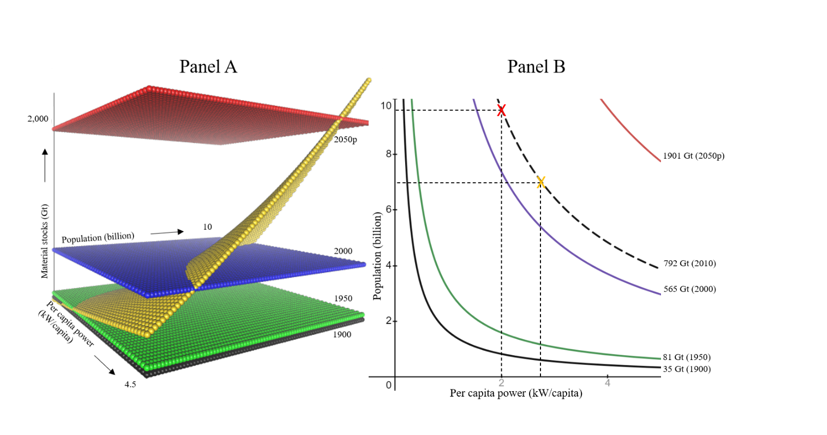
\includegraphics{fig/Leiva_Kleiber.png}

\emph{Figure: Panel A depicts Extended-Kleiber's Law relation between per capita power, population, and material
stocks. The yellow plane shows the 0.78 scaling of material stocks as a function of per capita power and
population. In 1900, a population of 1.6 billion people averaging 0.8 kW/capita implied material stocks of
35 Gt (black plane). In 1950, a population of 2.5 billion averaging 1.3 kW/capita implied materials stocks
of 81Gt (green plane). In 2000, a population of 6.1 billion people averaging 2.1 kW/capita implied
material stocks of 565 Gt (blue plane). In 2050, a projected 9.7 billion people averaging 4.0 kW/capita
implies material stocks of 1901 G (red plane). The rapidly increasing distance between the material stock
planes at equal 50-year intervals depicts the Great Acceleration. Panel B shows the intersections of the
yellow plane at each material stock plane of Panel A to depict iso-material stock curves: the
compensation between population and per capita power to maintain the respective material stock levels.
Note that these curves only show point estimates of the Extended Kleiber ́s Law and therefore need not
show the exact historical values of population and per capita power. The dashed-black line in Panel B
shows the 2010 iso-material stock curve (2010 level not shown in Panel A). The line depicts 792 Gt of
material stocks with 6.9 billion people averaging 2.8 kW/capita (orange marker, actual data for 2010 is
6.9 billion people averaging 2.3 kW/capita). The dashed-black line implies that maintaining Humanity's
materials stock at 792 Gt while growing to 9.7 billion people requires 2.0 kW/capita (red marker).}

If true, this relation implies a strict limit to power growth that cannot be addressed with low-carbon energy
sources.

Current projections of energy consumption and
population growth imply unsustainable levels of material stocks as they imply considerable additional
harvesting of the biosphere.

Current material stocks can be maintained while
accommodating population growth through 2050 if a 2.0 kW/capita limit is established. Although this
limit has been shown to be enough for a digni ed life, it implies a considerable degrowth in more than
half of the world ́s countries.

\emph{Theory}

Why do social systems ́ power and mass scale this way? One idea is based on fractal geometry (West et
al., 1999), where the invariant ``length'' could be given by the individual person. Brown et al.~(2011) use
this idea arguing that ``The energy and other resources that sustain these systems {[}animals and
economies{]} are supplied by hierarchically branching networks, such as the blood vessels and lungs of
mammals and the oil pipelines, power grids, and transportation networks of nations. Models of these
networks suggest that three-quarter-power scaling optimizes distribution of resources''. Another idea is
based on size-dependent limitation of resource storage (Maino et al., 2014; Thommen et al., 2019), where
the role of macromolecules could be played by energy goods. A third idea is based on the interaction of
physiological features with environmental conditions (Koziowski \& Weiner, 1997), where growth and
reproduction could be given by an economy ́s aggregate investment and consumption. In any case,
noting that the theoretical basis of Kleiber's Law remains controversial after 80 years of research (Escala,
2019; Hulbert, 2014), nding a theoretical explanation for an extended Kleiber ́s Law remains as future
research that may become foundational science towards Humankind ́s sustainability. In the meantime,
further data on mass and energy of nations is important to broaden the empirical basis of this
relationship.

If population reductions are not an option, the most reasonable response would be a worldwide 2.0
kW/capita limit.

A speci c limit at 2.0 kW/capita has been
proposed by the 2000-watt society since 1998 based on the per capita power of western Europe during
the 60s and the digni ed life it enabled, and according to our results, it is coincidentally the value required
to maintain material stocks in check below 800 Gt globally by 2050 given expected population levels.

\href{https://www.researchsquare.com/article/rs-66396/v2}{Leiva (2021) Why the energy transtition is not enough}
\href{pdf/Leiva_2021_Transition_not_enough.pdf}{(pdf)}

\href{https://en.wikipedia.org/wiki/Kleiber\%27s_law}{Kleiber's Law (Wikipedia)}

\hypertarget{energy-intensity}{%
\chapter{Energy Intensity}\label{energy-intensity}}

Energy intensity is a measure of the energy inefficiency of an economy. It is calculated as units of energy per unit of GDP.

\href{https://en.wikipedia.org/wiki/Energy_intensity}{Wikipedia}

GDP and energy consumption per capita variables are cointegrated and Granger
cause each other. First conclusion would be that energy consumption per capita
affects GDP per capita. In other words, a growth or reduce in energy consumption
will increase or decrease GDP. Energy consumption plays an important role on
economic growth, directly on labor and capital component and indirectly on
production process as well. Electric consumption is an incentive factor and indis-
pensable insurance for a sustainable economic growth. Second conclusion would be
that GDP per capita affects energy consumption per capita. That is, an increase or
decrease GDP per capita will increase or decrease energy consumption per capita.
Developing countries that are increasing their aggregate GDP and their production
are subject to demand more and more energy sources. Countries that are in short
providing the appropriate energy demand will be importing energy. This might
eventually cause current and trade deficit.

\href{https://www.researchgate.net/publication/316961845_Economic_Growth_and_Energy_Consumption_for_OECD_Countries}{Yildirim (2017) Economic Growth and Energy Consumption OECD}
\href{pdf/Yildirim_2017_Economic_Growth_and_Energy_Consumption_OECD.pdf}{(pdf)}

\hypertarget{power-density}{%
\section{Power Density}\label{power-density}}

\emph{Smil (Book)}

In this book, Vaclav Smil argues that power density is a key determinant of the nature and dynamics of energy systems. Any understanding of complex energy systems must rely on quantitative measures of many fundamental variables. Power density---the rate of energy flux per unit of area---is an important but largely overlooked measure. Smil provides the first systematic, quantitative appraisal of power density, offering detailed reviews of the power densities of renewable energy flows, fossil fuels, thermal electricity generation, and all common energy uses.

Smil shows that careful quantification, critical appraisals, and revealing comparisons of power densities make possible a deeper understanding of the ways we harness, convert, and use energies. Conscientious assessment of power densities, he argues, proves particularly revealing when contrasting the fossil fuel--based energy system with renewable energy conversions.

Smil explains that modern civilization has evolved as a direct expression of the high power densities of fossil fuel extraction. He argues that our inevitable (and desirable) move to new energy arrangements involving conversions of lower-density renewable energy sources will require our society---currently dominated by megacities and concentrated industrial production---to undergo a profound spatial restructuring of its energy system.

\href{https://mitpress.mit.edu/books/power-density}{Vaclav Smil (2015) Power Density (Book)}

\emph{Smil (Primer)}

Many factors combine to determine their technical difficulty, their cost and their environmental
impacts. A great deal of attention has been recently paid to the pace of technical innovation
needed for the shift from the world dominated by fossil fuel combustion to the one relying
increasingly on renewable energy conversions, to the likely costs and investment needs of this
transitions, and to its environmental benefits, particularly in terms of reduced CO 2 emissions.
Inexplicably, much less attention has been given to a key component of this grand transition, to
the spatial dimension of replacing the burning of fossil fuels by the combustion of biofuels and
by direct generation of electricity using water, wind, and solar power. Perhaps the best way to
understand the spatial consequences of the unfolding energy transition is to present a series of
realistic power density calculations for different modes of electricity generation in order to make
revealing comparisons of resources and conversion techniques. Detailed calculations will make it
easy to replicate them or to change the assumptions and examine (within realistic constraints)
many alternative outcomes.

\textbf{Energy Density vs Power Density}

\emph{Energy density} is easy -- power density is confusing. Energy density is simply the amount of
energy per unit weight (gravimetric energy density) or per unit volume (volumetric energy
density). With energy expressed (in proper scientific terms) in joules or less correctly in calories
(and in the US, the only modern state that insists on using outdated non-metric measures, in
BTUs), with weight in grams (and their multiples), and with volume in cubic centimeters, liters
(dm 3 ) or cubic meters, energy density is simply joules per gram (J/g) or joules per cubic
centimeter (J/cm 3 ) or, more commonly, megajoules per kilogram (MJ/kg) and megajoules per
liter (MJ/L) or gigajoules per ton (GJ/t) and gigajoules per cubic meter (GJ/m 3 ).

\emph{Power density} is a much more complicated variable.
Power density expressed as energy flux per unit of horizontal surface universal.
\(W/m^{2}\) of horizontal area of land or water
surface has been receiving more attention because of the growing interest
in renewable energy resources and their commercial conversions to fuels and electricity.
Invariably, power densities of these stocks
and flows are considerably lower than power densities and uses of fossil fuels, those highly
concentrated stores of ancient photosynthetic production -- and these differences are a key factor
in determining the potential contribution of renewable energies to the world's future fuel and
electricity supply.

\begin{longtable}[]{@{}lrl@{}}
\caption{Low-High Power Density estimate}\tabularnewline
\toprule
Power Source & Power & Density (\(W/m^{2}\))\tabularnewline
\midrule
\endfirsthead
\toprule
Power Source & Power & Density (\(W/m^{2}\))\tabularnewline
\midrule
\endhead
Natural Gas & 200 & 2000\tabularnewline
Coal & 100 & 1000\tabularnewline
Solar (PV) & 4 & 9\tabularnewline
Solar (CSP) & 4 & 10\tabularnewline
Wind & 0.5 & 1.5\tabularnewline
Biomass & 0.5 & 0.6\tabularnewline
\bottomrule
\end{longtable}

Implications of these differences are manifold. Changing the power density-determined
infrastructure of energy systems that were created over more than a century for electricity
generation from fossil fuel combustion will not be easy. A fossil-fuelled civilization has been
securing the supply of its most flexible form of energy by ``shifting downward,'' that is by
generating electricity with power densities 1-3 orders of magnitude higher than the common
power densities with which electricity is used in buildings, factories and cities. In a civilization
that would rely only on renewable energy flows, but that would inherit today's urban and
industrial systems, we would produce electricity at best with the same power densities with
which they would be used --- but more often we would have to concentrate diffuse flows of solar
radiation, wind, and biomass in order to bridge power density gaps of 2-3 orders of magnitude.
This new energy infrastructure would increase fixed land requirements and preempt any other
form of land use in areas devoted to PV cells, heliostats or fast-growing wood plantations. Most
of the area occupied by large wind farms could be used for crops or grazing but other land uses
would be excluded, and large areas dotted with wind turbines would require construction and
maintenance of access roads as well as the creation of buffer zones not suitable for permanent
human habitation. And in all cases of renewable energy conversion, much more land would be
needed for more extensive transmission rights-of-way in order to export electricity from sunny
and windy regions, or from areas suited for mass-scale biomass production, to major urban and
industrial areas.

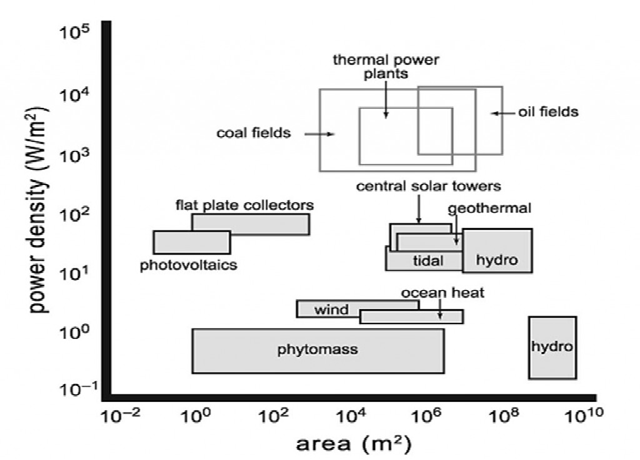
\includegraphics{fig/smil_power_densities.png}

Figure: Power densities of fossil fuel extraction, thermal electricity
generation and renewable modes of electricity production.

As a result, these new energy infrastructures would have to be spread over areas ten to a
thousand times larger than today's infrastructure of fossil fuel extraction, combustion and
electricity generation: this is not an impossible feat, but one posing many regulatory
(environmental assessments of affected areas, rights-of-way permission and inevitable lawsuits),
technical and logistic challenges. Higher reliance on renewable energies may be desirable
(mainly because of perceived environmental and strategic reasons) and technical advances
would also make it an increasingly appealing economic choice --- but inherently low power
densities of these conversions will require a new system of fuel and electricity supply that will be
able to substitute for today's dominant practices only after decades of gradual development.

\href{pdf/smil_2010_power_density_primer.pdf}{Vaclav Smil (2010) Power Density Primer (pdf)}

\hypertarget{energy-development}{%
\chapter{Energy Development}\label{energy-development}}

Energy development is the field of activities focused on obtaining sources of energy from natural resources. These activities include production of conventional, alternative and renewable sources of energy, and for the recovery and reuse of energy that would otherwise be wasted. Energy conservation and efficiency measures reduce the demand for energy development, and can have benefits to society with improvements to environmental issues.

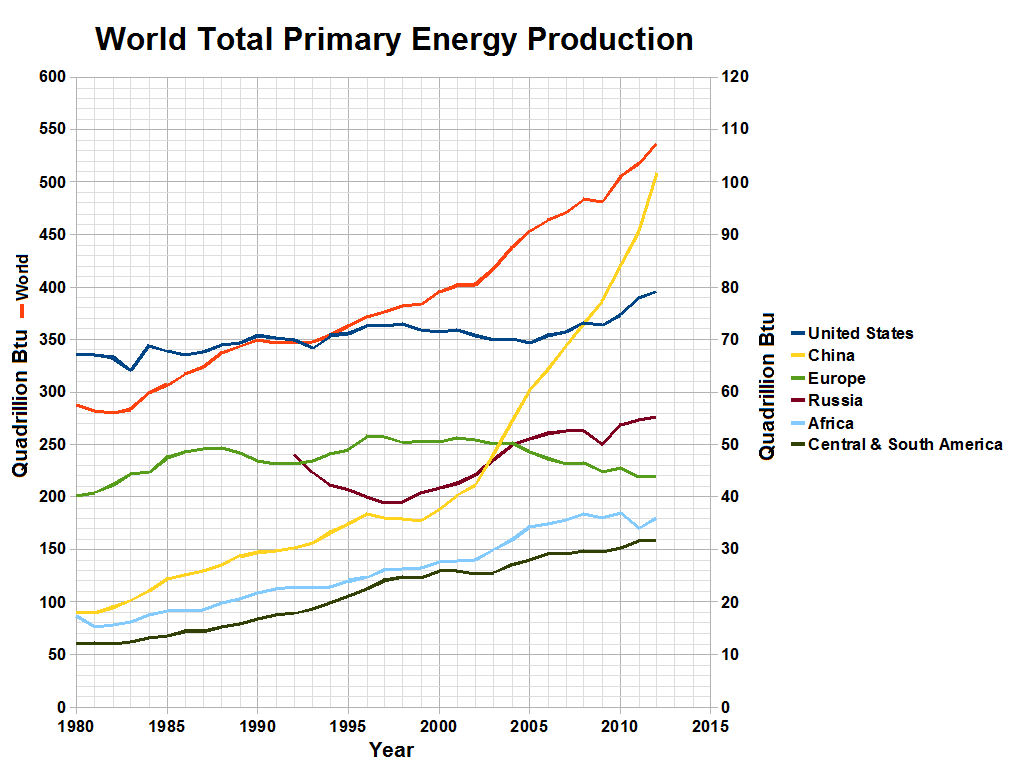
\includegraphics{fig/WP_World_total_primary_energy_production.png}

Figure: World total primary energy production in quadrillion Btu.
Note: world total on left y-axis, while
regional figures are shown on right y-axis
(approx. figures in parenthesis for 2010 and 2011, respectively).

World (510)
China (97)
United States (78)
Russia (56)
Europe (45)
Africa (37)
Central and South America (30)

\href{https://en.wikipedia.org/wiki/Energy_development}{Wikipedia}

Conversion:
1 Btu = 0.00029329722222222 kWh

1 qudrillion = \(10^{15}\)

\href{https://www.unitjuggler.com/convert-energy-from-Btu-to-kWh.html}{unitjuggler}

\hypertarget{energy-transition}{%
\chapter{Energy Transition}\label{energy-transition}}

\emph{Thompson}

Vaclav Smil has repeatedly pointed out that
a green energy revolution would be qualitatively different than any energy change in human history
because it involves moving from more concentrated to less concentrated energy,
rather than in the opposite direction.

However much companies and governments promise dramatic and rapid change, their deeds and small-print rhetoric point to the hard consequences of this reality.

BP may be heralding a low carbon energy future, but its own 2020 annual report presumes the world will still be using between 80 and 100 million barrels of oil a day in 2040. The same report says that `significant levels of investment are required for there to be sufficient supplies of oil to meet demand in 2040.' It takes some cognitive dissonance to believe this oil could still be produced whilst investors shut capital out of the privately-owned oil industry; that is, unless it is accepted that all future oil comes from Russia's Rosneft and the Middle Eastern state-owned oil companies and is so expensive as to act as an impediment to growth. Still owning 19.75 per cent of Rosneft, BP has clearly hedged how it thinks the energy future will play out.

To think about the energy-origins of western prosperity opens up difficult truths about the place of European empire and the United States' Middle Eastern wars in the economic history of the twentieth and early twenty-first century. Part of climate idealism contains a desire to leave this unpalatability behind, replacing fossil-fuel imperialism with climate justice. But after the Second World War, western economic life depended on the oil that came out of the Persian Gulf, through the Suez Canal, and into pipelines running to the Mediterranean. The counter-factual that eliminates past wrongs takes a lot else with it, including that which most people in western democracies have little inclination to forsake. Given that battery production presently relies on cobalt mining done in grim conditions in the Democratic Republic of Congo, sometimes with child labour, and much of the solar-grade polysilicon used in solar panels is produced in Xinjiang, green energy will bring less ethical relief than often supposed.

Our cognitive struggles with energy matters extend to our concepts of historical time. Both the dread of a coming apocalypse and a faith in endless human innovation and moral improvement appear hardwired into western culture, first from Christianity, and then its secular offshoot the Enlightenment. When confronted with collective existential questions, western minds reach rather easily to millenarian fears and hopes. Christianity began, after all, with the expectation of an apocalypse and the imminent arrival of God's kingdom. Although the Roman Catholic Church made Latin Christianity worldly, and Augustine slammed down millenarianism as delusional, the original Christian spirit lingered, readily available as a lens to give moral meaning to past sins in times of social and economic crisis. The apparent ideational clarity of the apocalyptic moment now permeates radical climate activism, captured in Extinction Rebellion's name, as well as the movement's performative, and at times itinerant, political style.

\href{https://engelsbergideas.com/essays/the-geopolitical-fight-to-come-over-green-energy/}{Helen Thopmson}

\emph{Tooze}

Net-zero at zero net cost?

The big question is thus not how to mobilise the new money but how to ensure investment happening anyway flows in the right direction. McKinsey trumpets the conclusion that the overall cost to the EU of achieving net-zero by 2050 will be zero: energy savings will cover the costs of the investment. This is great news.

But, as McKinsey knows only too well, that is not how trillions of investment are normally justified. They have to produce an adequate rate of return---opportunity cost is the measure that matters. It is a matter not of physical contraints but of political economy and on that score the news is less good.

According to McKinsey, between now and 2050, almost half the necessary investment will not meet standard investment criteria. Up to 2030, due to the high cost of renewable technologies in their early stages, less than 40 per cent will be justifiable on commercial grounds. In industry and buildings, two sectors where emissions are hard to abate, a tiny fraction of the necessary investment will generate an adequate profit.

It is in closing the gap between the investment that McKinsey has defined as necessary and that which it has defined as justifiable from a business point of view that government comes in.

If the gap were to be closed by public expenditure, Europe's governments would, according to McKinsey, need to mobilise €4.9 trillion in subsidies over 30 years. That is the amount of profit taxpayers would need to offer investors to get them interested in the energy transition---€365 for every man, woman and child in the EU27, every year for 30 years. Painful and unfair, no doubt, but hardly inconceivable.

In any case, the public purse is only one way of driving business investment. An alternative is to use carbon pricing. McKinsey estimates that with a carbon price of €100 per ton 80 per cent of the necessary investment could be justified on commercial grounds. The funds generated from an emissions-trading system could then be recycled in subsidies and other promotional spending. In hard-to-abate sectors, direct interventions would remain indispensable.

\href{https://adamtooze.substack.com/p/chartbook-newsletter-17}{Adam Tooze}

\hypertarget{minerals-in-transition}{%
\section{Minerals in Transition}\label{minerals-in-transition}}

\emph{CarbonTracker on IEA Study}

The IEA's latest piece on minerals{[}1{]} critical to the energy transition gives a rather pessimistic spin to what was some very positive data. Looked at from a wider perspective, the note provides another useful source of analytical support for the energy transition.

The IEA looked into the amount of minerals needed to fuel the energy transition, and pretty quickly worked out `there is no shortage of resources'. The world has plenty of lithium, nickel, rare earth metals and so on. This is what the United States Geological Survey (USGS) has been saying for a while,{[}2{]} and fits with the work done by the Energy Transitions Commission{[}3{]} on mineral availability.

The IEA notes for example that we have 170 times as much lithium reserves as annual demand and that our lithium reserves have increased by 42\% over the last eight years as higher prices and the prospect of rising demand have drawn out new investment. Under the IEA's 1.5 degrees scenario, we will need about twice the amount of critical minerals by 2040 (six times as much for the clean energy industry, but that is only part of global demand), and the IEA put forward a series of sensible suggestions (increase recycling, invest in new supply and so on) to ensure that we get it.

However, their take then turns gloomier as we are warned about how hard this is going to be. Impressive charts show that the average electric vehicle uses 210kg of critical minerals compared to only 35kg for an ICE car and that a MW of solar generation capacity needs 6.5 tonnes of critical minerals compared to a coal plant which needs only 3 tonnes. We are then encouraged to think about all the ESG issues and environmental issues associated with the surge in mineral usage and to worry about supplier concentration, water usage, pollution and depletion.

Stand back a moment however, and you can see immediately that the IEA are very selective in their presentation of the data. They look only at the stocks (the assets you need to build the generator or car) not the flows (the energy you need to run them). But the flows of energy are 2-3 orders of magnitude larger than the stocks, and this means that many of their conclusions are more useful for fossil fuel advocates than for policymakers.

One way to demonstrate this is to look at the weight of the material that is required for a fossil fuel system versus a renewable system, as weight is a pretty good proxy for environmental impact. All that coal and oil has to be extracted and converted and shipped around, and at every stage it requires complex and heavy equipment which has an impact on communities and air quality. So we take IEA data to compare below the critical mineral requirement of the renewable system with the energy requirement of the fossil system, to get a more appropriate comparison. There are of course other materials like steel and cement to consider when building transition infrastructure, and other areas like transport networks, but it is safe to say that these will weigh considerably more for the heavy molecules of the fossil system than the light electrons of the renewable system.

For example, take those 6.5 tonnes (half of it from silicon which is not exactly a rare mineral) that you need to build 1MW of solar capacity. It turns out that this is an absolutely immaterial number compared to the weight of the coal that is used to generate electricity. Over its lifetime of 30 years, 1MW of solar capacity will generate over 40,000 MWh of electricity, so the mineral requirement is just 0.15kg per MWh. Compare that to a coal fired generation station where the critical mineral requirement is indeed a bit less, but you need 350 kg of coal to generate that MWh.{[}4{]} On this calculation, coal generation will need more than 2,000 times more material by weight than solar generation.

It is a similar story in the transport sector. The average car uses about a tonne of oil a year, or 15 tonnes over its lifetime. Compare that with the 210kg of critical minerals that the EV needs and the weight of the oil is 71 times higher than the weight of the minerals. You burn the oil only once, but the minerals can and will be recycled many times.

\href{https://carbontracker.org/mineral-constraints-for-transition-overstated-by-iea/}{carbonTracker}

\emph{IEA Study}

Minerals are essential components in many of today's rapidly growing clean energy technologies -- from wind turbines and electricity networks to electric vehicles. Demand for these minerals will grow quickly as clean energy transitions gather pace. This new World Energy Outlook Special Report provides the most comprehensive analysis to date of the complex links between these minerals and the prospects for a secure, rapid transformation of the energy sector.

Alongside a wealth of detail on mineral demand prospects under different technology and policy assumptions, it examines whether today's mineral investments can meet the needs of a swiftly changing energy sector. It considers the task ahead to promote responsible and sustainable development of mineral resources, and offers vital insights for policy makers, including six key IEA recommendations for a new, comprehensive approach to mineral security.

\href{https://www.iea.org/reports/the-role-of-critical-minerals-in-clean-energy-transitions}{IEA Study}
\href{pdf/IEA_2021_Minerals_Energy_Transitions.pdf}{(pdf)}

\hypertarget{iea-net-zero-2050}{%
\section{IEA Net-zero 2050}\label{iea-net-zero-2050}}

\emph{Jeff St.~John}

Net-zero carbon emissions by 2050 --- but only if governments redouble their efforts, all fossil fuel investment is halted, and renewable energy capacity and and infrastructure are added at unprecedented scale

Over the next decade, \$5 trillion must be invested in converting energy used for electricity generation, transportation, industry and buildings from fossil fuels to carbon-free sources. It will entail a colossal undertaking that will require far greater commitments from government and industry than have been made thus far. But it could \emph{drive massive economic growth} in rich and poor countries alike, the report finds.

On the electricity front, solar power will need to reach 630 gigawatts and wind power 390 gigawatts by 2030, representing annual additions at four times the scale of the deployment record set in 2020. Annual investment in transmission and distribution grids to manage these renewable resources must triple from \$260 billion today to \$820 billion by decade's end.

On the transportation front, sales of new internal combustion cars must end and be replaced by electric vehicles or other carbon-free models by 2035. Public EV charging points must grow from around 1 million today to 40 million in 2030, at a cost of about \$90 billion. Manufacturing capacity for batteries for this EV fleet will need to grow from 160 gigawatt-hours to 6,600 GWh by 2030, or the equivalent of nearly 20 gigafactories being added each year.

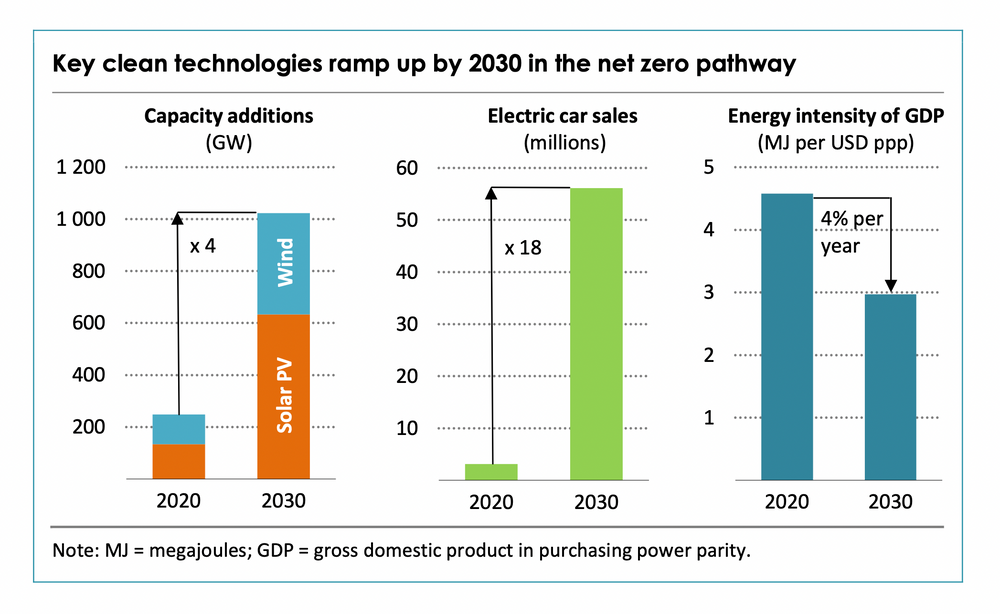
\includegraphics{fig/clean_technology_ramp-up_2030.png}

Energy efficiency improvements must average 4 percent per year through decade's end, roughly three times the rate achieved over the past two decades. And approximately \$40 billion per year must be invested to bring electricity to about 785 million people and clean cooking solutions to about 2.6 billion people

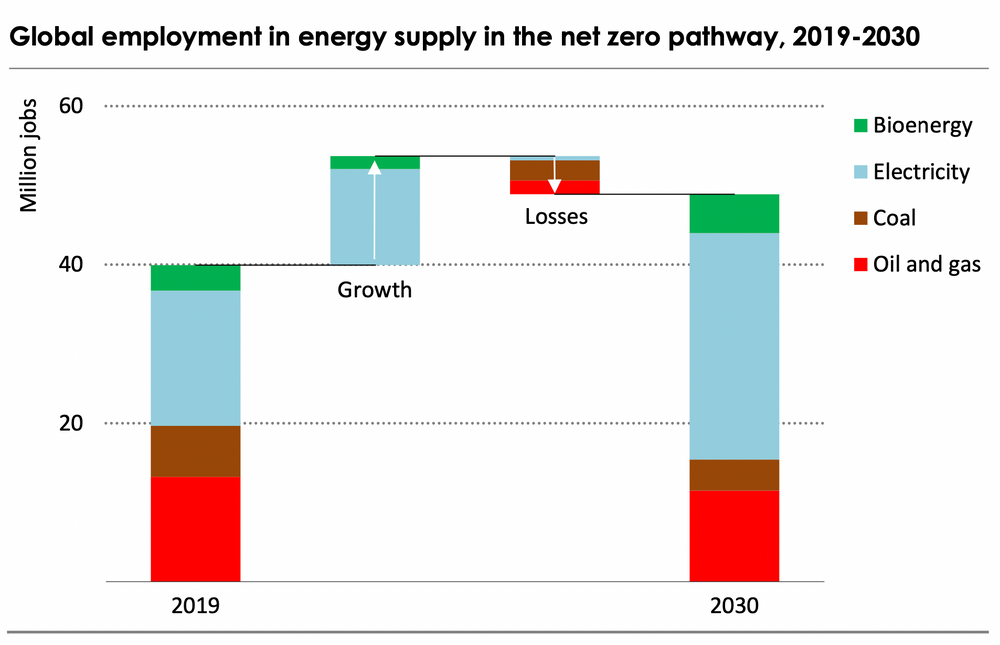
\includegraphics{fig/clean_technology_ramp-up_employment_2030.png}

\href{https://www.canarymedia.com/articles/iea-world-is-on-the-knifes-edge-of-reaching-net-zero-carbon-by-2050/}{Jeff St.~John}

\href{https://www.iea.org/reports/net-zero-by-2050}{IEA (2021) Net-Zero 2050 Study}

\emph{Hickel on IEA}

The new IEA report on net-zero is a big step in the right direction, and its call to cease all new fossil fuel projects has grabbed headlines, which is welcome. But the report also has some serious problems that are worth discussing:

First, in order to maintain the assumption of economic growth-as-usual in rich countries, it relies on unprecedented rates of GDP/energy decoupling, to an extent that has been questioned repeatedly in the empirical literature.

Second, it achieves this decoupling in large part by relying on efficiency improvements, but the model does not take adequate account of rebound effects, which have been identified as a significant problem.

Third, it relies on a lot of BECCS and other carbon capture and storage approaches, which is a risky gamble and has several big downsides (in terms of land use, biodiversity loss, soil depletion, competition with food crops, energy and water use, etc.)

If we dial down our assumptions about decoupling, bioenergy and CCS to safer and more feasible rates, the net-zero pathway will require a bigger reduction of energy and resource use in rich countries. This needs to be part of our discussion.

For a review of evidence related to the three points above, and for a discussion of more technologically feasible approaches, \href{https://www.nature.com/articles/s41467-021-22884-9}{this recent paper} by \citet{LorenzClimate} and Manfred Lenzen is useful.

\href{https://twitter.com/jasonhickel/status/1394940762891169794}{Hickel (twitter thread) On IEA}

\emph{Keyzer \& Lensen }

1.5  °C scenarios reported by the Intergovernmental Panel on Climate Change (IPCC) rely on combinations of controversial negative emissions and unprecedented technological change, while assuming continued growth in gross domestic product (GDP). Thus far, the integrated assessment modelling community and the IPCC have neglected to consider degrowth scenarios, where economic output declines due to stringent climate mitigation. Hence, their potential to avoid reliance on negative emissions and speculative rates of technological change remains unexplored. As a first step to address this gap, this paper compares 1.5  °C degrowth scenarios with IPCC archetype scenarios, using a simplified quantitative representation of the fuel-energy-emissions nexus. Here we find that the degrowth scenarios minimize many key risks for feasibility and sustainability compared to technology-driven pathways, such as the reliance on high energy-GDP decoupling, large-scale carbon dioxide removal and large-scale and high-speed renewable energy transformation. However, substantial challenges remain regarding political feasibility. Nevertheless, degrowth pathways should be thoroughly considered.

The results indicate that degrowth pathways exhibit the lowest
relative risks for feasibility and sustainability when compared
with established IPCC SR1.5 pathways using our socio-technical
risk indicators. In comparison, the higher the technological reli-
ance of the assessed mitigation pathways, the higher the risks for
socio-technical feasibility and sustainability. The reverse is likely
the case for socio-political feasibility, which, however, is softer
than socio-technical feasibility. This result contrasts strongly with
the absolute primacy of technology-driven IAM scenarios in the
IPCC SR1.5.

\citep[ 1.5 °C degrowth scenarios suggest the need for new mitigation pathways]{LorenzClimate}(\url{https://www.nature.com/articles/s41467-021-22884-9})
\href{pdf/Keyser_2021_New_Mitigation_Pathways.pdf}{(pdf)}

\emph{Fickling}

One thing worth noting about the radical-sounding \citet{iea}
announcement that no new petroleum fields need to be developed any more --- this is more or less the lived reality of oil majors right now, and has been for years.

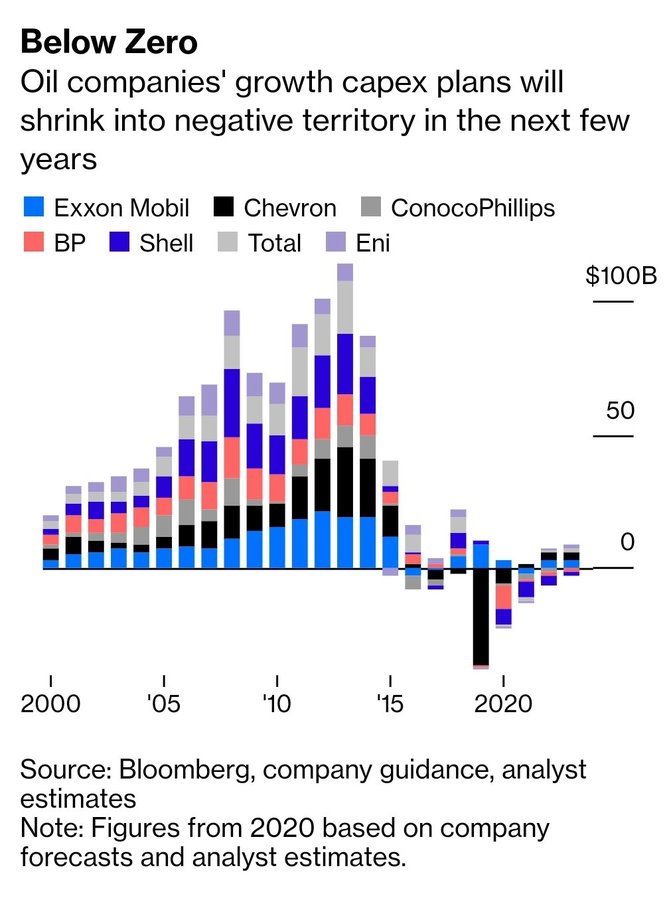
\includegraphics{fig/big_oil_investments.jpeg}

Big Oil stopped investing growth capex around 2016.

\href{https://twitter.com/davidfickling/status/1394810455655280640}{Fickling (twitter thread)}

\hypertarget{transition-risks}{%
\section{Transition Risks}\label{transition-risks}}

\textbf{Unrealistic Scenario Pathways}

\emph{Keyser}

1.5 °C scenarios reported by the Intergovernmental Panel on Climate Change (IPCC) rely on
combinations of controversial negative emissions and unprecedented technological change,
while assuming continued growth in gross domestic product (GDP). Thus far, the integrated
assessment modelling community and the IPCC have neglected to consider degrowth sce-
narios, where economic output declines due to stringent climate mitigation. Hence, their
potential to avoid reliance on negative emissions and speculative rates of technological
change remains unexplored. As a first step to address this gap, this paper compares 1.5 °C
degrowth scenarios with IPCC archetype scenarios, using a simplified quantitative repre-
sentation of the fuel-energy-emissions nexus. Here we find that the degrowth scenarios
minimize many key risks for feasibility and sustainability compared to technology-driven
pathways, such as the reliance on high energy-GDP decoupling, large-scale carbon dioxide
removal and large-scale and high-speed renewable energy transformation. However, sub-
stantial challenges remain regarding political feasibility. Nevertheless, degrowth pathways
should be thoroughly considered.

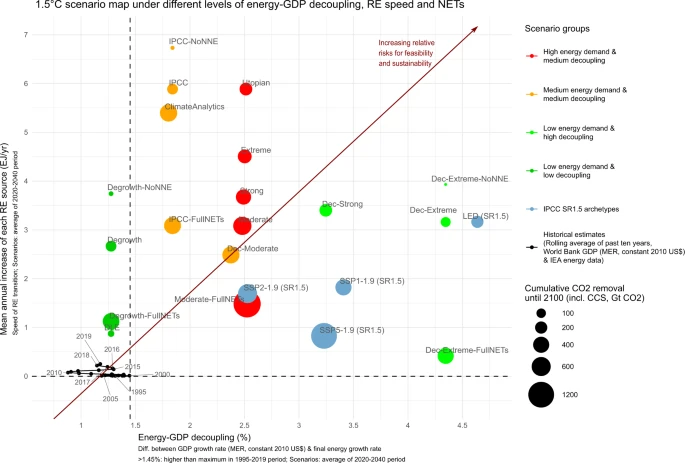
\includegraphics{fig/transition_presumptions.png}

\emph{Figure: 1.5 °C scenario map under different levels of energy-GDP decoupling, RE speed and NETs.
The dimensions are `speed of renewable energy transition'
(for the scenarios the 2020--2040 annual average growth in solar, wind and other renewables, in EJ/yr),
`energy-GDP decoupling' (for the scenarios the 2020--2040 average difference between GDP growth rate and final energy growth rate, in \%) and cumulative CO 2 removal until 2100,
including CCS (GtCO 2 ).
Historical data points are the rolling averages of the past ten years (e.g., for the 1995 point the period 1986--1995) of the respective indicators.
This averaging was chosen (1) because GDP and final energy data are noisy and (2) to emphasise longer-term trends.
While historically four years were above a decoupling of 2\% since 1986, these are outlieres around a lower, almost constant trend.
Historical GDP data (MER, constant 2010 US\$) is taken from the World Bank.}

\href{https://www.nature.com/articles/s41467-021-22884-9}{Keyser (2021) 1.5 °C degrowth scenarios suggest the need for new mitigation pathways}
\href{pdf/Keyser_2021_New_Mitigation_Pathways.pdf}{(pdf)}

\textbf{Unrealistic Assumptions}

Existing plans to limit global warming rely too much on ``increasingly unrealistic assumptions'' that societies will be able to remove huge amounts of carbon from the atmosphere while simultaneously maintaining incessant economic growth over the next 50 years, according to a May 2021 study in Nature Communications. These strategies appear to be speeding the planet deeper into the climate crisis.

Economic degrowth---strategies to shrink the economies of rich, developed countries while maintaining the wellbeing of the people and environments they are based on---might be less risky, and a better way to meet the goals of the Paris climate agreement. Efforts to slow climate change that are built on structural social changes, like rethinking the way we work, produce food, heat our homes and move around could be more successful than those that rely on uncertain carbon removal technologies.

The over-reliance on unprecedented carbon dioxide removal and energy efficiency gains means we risk catastrophic climate change if one of the assumptions does not materialize.

\href{https://insideclimatenews.org/news/18062021/degrowth-economies-climate-change-technology-gdp/}{InsideClimateNews}

\hypertarget{batteries}{%
\chapter{Batteries}\label{batteries}}

The battery market has seen dozens of chemistries come and go, but four have stuck and scaled to achieve mass-market penetration: lead acid, nickel-cadmium (Ni-Cd), nickel-metal hydride (NiMH) and lithium-ion (Li-ion).

Most of the developing world still uses lead-acid batteries, a \$45 billion global market. But lithium-ion batteries have been gaining ground rapidly in wealthy markets.

LIBs have hit on a combination of anode, cathode and electrolyte that performs well enough along several criteria (especially cost) to work for most short-duration applications today. They have become cheap, and manufacturing capacity has converged around them.

\href{https://www.canarymedia.com/articles/the-basics-of-how-lithium-ion-batteries-work/}{Roberts}

\hypertarget{lithium}{%
\section{Lithium}\label{lithium}}

\hypertarget{portugals-lithium-reserves}{%
\subsection{Portugal's Lithium Reserves}\label{portugals-lithium-reserves}}

According to the European commission, Europe will need 60 times more lithium by 2050 (target year for carbon neutrality) for electric cars and energy storage alone, which is fueling an international race to extract lithium from the different sources where such deposits can be found, such as hard rocks, salt brines and geothermal water.

But for the people of Covas do Barroso, this scramble for raw materials and the prospect of an open-air mine translate into fears of deforestation, air pollution, water contamination, noise and an end to their way of life.

Interviews conducted by Euronews with a dozen residents, revealed that the vast majority of them were against mining lithium from the mountain rocks near their village, while a few were indifferent. No one was in favour.

``I think it won't bring anything good,'' said Paulo Pires, a local shepherd. ``It will consume a lot of water, which we need for the sheep and for their fields. Instead of hearing birds, I will hear explosions, machines\ldots there will be a lot of pollution.''

``I'm not against lithium. But I'm not in favour of polluting my village and other villages like mine in order to depollute cities'' Pires added.

A study by the Portuguese University of Minho, conducted for Savannah Resources, found that Portugal's 60,000 tons of known lithium reserves (0,4\% of world's reserves) are ``insufficient to meet the demand for lithium derivatives for the production of batteries in Europe''. However, the report also adds that these reserves ``are very relevant in reducing Europe's dependence on other regions of the globe and increasing the security of Europe's supply chain.''

\href{https://www.euronews.com/2021/04/23/portuguese-village-suffers-the-high-cost-of-low-carbon-energy}{Euronews}

\hypertarget{lithium-ion-batteries-libs}{%
\section{Lithium-ion Batteries (LIBs)}\label{lithium-ion-batteries-libs}}

\emph{Roberts}

The global market for EV batteries alone is expected to hit almost \$1 trillion by 2030.
The more energy-dense, cheap and safe LIBs can get, the faster the electrification of transportation will happen.
LIBs are being used both for distributed, building-level energy storage and for large, grid-scale storage installations.

The global storage market is expected to grow at an average of 31 percent a year over the coming decade, reaching 741 gigawatt-hours of cumulative capacity by 2030.
The vast bulk of the demand for batteries is going to come from transportation

In 2019, the three chemists behind the initial development of lithium-ion technology won the Nobel Prize in chemistry. LIBs boast incredibly high energy density and specific energy, which is to say, they cram lots of oomph into a small, lightweight package, and they are capable of cycling many more times than their predecessors.

Lithium-ion battery pack prices, which were above \$1,100 per kilowatt-hour in 2010, have fallen 89\% in real terms to \$137/kWh in 2020. By 2023, average prices will be close to \$100/kWh.
With foreseeable improvements in LIB chemistry, prices could hit \$40 or even \$30/kWh in coming decades.
LIBs are going to hit limits, even if it's just the base price of raw materials, before they become economical for long-duration grid storage. They are being installed for 4- to 6-hour storage applications, sometimes 8 hours, and someday may even aspire to 12 hours. But beyond that --- for the weekly or even seasonal storage a renewables-based grid will need --- some other technology or technologies will have to step in.

Before Tesla was founded, Li-ion batteries were almost exclusively used in consumer electronics --- mainly laptops and cell phones. At the time of the launch of the Tesla Roadster in 2008, the total global Li-ion manufacturing capacity was approximately 20 GWh per year. By 2030, we expect over 2,000 GWh of annual production capacity based on already announced plans by cell manufacturers.
That would be 100× growth in 22 years.

LIBs do face restraining pressures, especially materials and safety concerns.

\href{https://www.canarymedia.com/articles/why-lithium-ion-batteries-are-so-important/}{Roberts}

LIBs have been around in commercial form since the early 1990s, though obviously they've improved quite a bit since then.

Today's most common and popular LIBs use graphite (carbon) as the anode, a lithium compound as the cathode and some organic goo as an electrolyte. They boast two key advantages over prior battery chemistries.

First, they need very little electrolyte. They are what's known as ``intercalation'' batteries, which means the same lithium ions nestled (intercalated) in the structure of the anode transfer to be intercalated in the cathode during discharge. The electrolyte only has to serve as a conduit; it doesn't have to store many ions. Consequently, the cell doesn't need much of it. Saving on electrolyte saves space and weight. (Bonus: The process is almost perfectly reversible, which gives LIBs their high cycle life.)

Second, LIBs squeeze lots of energy into a small space. Lithium is the lightest metal (at the upper left corner of the periodic table) and extremely energy-dense, so LIB cells can work with electrodes only 0.1 millimeters thick. (Compare lead-acid electrodes, which are several millimeters thick.) This also makes LIBs smaller and lighter.

Even the biggest grid battery is just stacks upon stacks of cells, like Lego bricks. LIBs are extremely modular --- they can be scaled precisely to need.

The most common LIB chemistries used today are lithium nickel manganese cobalt oxide (NMC) and lithium nickel cobalt aluminum (NCA), which use compounds of those metals as the cathode. Lithium and nickel turn out to be a knockout combo: light and energy-dense.

Some batteries, particularly those with cobalt, are prone to ``thermal runaway,'' which means that if one cell goes haywire and heats up, it heats up the next one, and so on and so on in a self-reinforcing process that results in fires

List of LIB chemistries:

\begin{verbatim}
Lithium nickel manganese cobalt oxide (NMC cathode)
Lithium nickel cobalt aluminum (NCA cathode)
Lithium ferro phosphate or lithium iron phosphate (LFP cathode)
Lithium manganese oxide (LMO cathode) and lithium manganese nickel oxide (LMNO cathode)
Lithium sulfur (Li-S, sulfur cathode)
Lithium metal (anode) and solid state
Lithium titanate (LTO anode)
Lithium air (Li-air, lithium anode)
\end{verbatim}

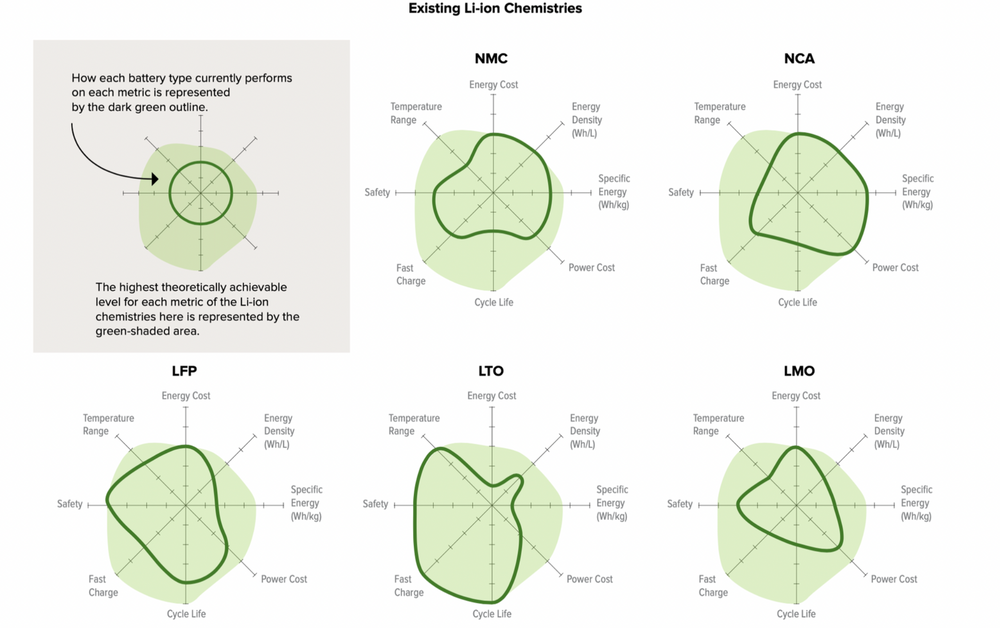
\includegraphics{fig/LithiumIon_chemistries.png}

Cobalt, used in standard NMC and NCA chemistries, is highly toxic, comes almost entirely from the Democratic Republic of the Congo, and is mined in terrible working conditions that frequently spur charges of human rights abuses. Nickel and lithium are less nasty in and of themselves, but they may run into supply constraints as the market grows. (Nickel, in particular, is a \href{https://www.bbc.com/news/business-56288781}{source of current stress}.)

Smart manufacturers such as Tesla and others are diversifying their battery lines in anticipation of supply issues, trying to evolve away from cobalt and attempting to secure a steady supply of lithium and nickel.

\href{https://www.canarymedia.com/articles/the-basics-of-how-lithium-ion-batteries-work/}{Roberts}

\textbf{Sionic}

Sionic is betting that its approach will prove to be easier and cheaper to adopt for the companies that have already sunk massive investment into their factories.

Instead of re-engineering silicon to tamp down on its propensity to expand and contract during cycling, Sionic uses low-cost micron silicon and designs around that property.

``If you fight physics, physics always wins,'' said Sionic CTO Surya Moganty. ``We are controlling, or engineering, that expansion of silicon so it does not cause problems.''

Sionic also leans on its corporate pedigree to design an electrolyte that's optimized for safe performance with the new anode. That's important, because changing one key component of a battery typically affects how the other pieces perform.

\href{https://www.canarymedia.com/articles/startup-sionic-promises-next-gen-battery-benefits-without-the-wait/}{Spector/Canary}

\textbf{Lition-ion Varieties}

There are a few clear leaders --- lithium nickel manganese cobalt oxide (NMC), lithium nickel cobalt aluminum (NCA), and lithium ferro phosphate (LFP).

Most EV makers use NMC batteries; Tesla uses NCA. In the past, it's been difficult to push down the amount of cobalt in these batteries (it plays an important balancing role), but manufacturer LG recently introduced an NMC 811 battery: 80 percent nickel, 10 percent manganese, 10 percent cobalt. GM will use them in its new line, including in the Hummer, and Tesla will put them in some of its Model 3s in China.

Most big battery manufacturers, including Panasonic (which supplies many of Tesla's batteries), have vowed to gradually reduce and eventually eliminate cobalt.

Nickel is the key to energy density. Tesla, VW, and others are working on special high-nickel battery varieties that will be used for specialty vehicles that require extra-high energy density, like larger SUVs and trucks.

But not every vehicle needs that, and nickel supply constraints are looming, so work is also being done to further boost manganese --- a much more stable, abundant material --- and reduce cobalt.

\textbf{Silicon Anodes}

Many LIB developers are experimenting with silicon as an anode coating, partially or completely replacing graphite.

Silicon holds on to nine times more lithium ions than graphite, so energy density improves (range expands by 20 percent), and a silicon battery can charge and discharge much more quickly than graphite batteries, so power density improves as well. But silicon expands when it absorbs ions, so it breaks down quickly; cycle life is still much lower than graphite.

Automotive cells with NCA or NCM cathodes paired with Si-dominant anodes will increase energy density by up to 50\%, thereby dropping the \$/kWh cost by 30-40\% in less than a decade.

Silicon-as-anode doesn't operate via intercalation. Instead of nestling into the anode, ions react with the silicon and bond with it, a process called ``conversion.'' That makes it more difficult to peel the ions off without damage, but it can hold way more ions.

\textbf{Fluorides Cathodes}

Metal fluoride-based cathodes (like iron fluoride or copper fluoride) and sulfur-based cathodes --- which also operate via conversion rather than intercalation and can also store more ions.

It's plausible that with a conversion cathode and an engineered low-swell silicon anode, the cycle life of Li-ion can be extended all the way to 10,000 full cycles while also having the highest energy density.

Only that combination --- a conversion-based anode and a conversion-based cathode --- that can bring LIB prices down to ``\textasciitilde\$50/kWh by 2030 and \textasciitilde\$30/kWh by 2040.

\textbf{Lithium ferro phosphate (LFP)}

LFP use a lithium-iron compound as cathode.

A few years ago, it looked like LFPs were going to be displaced by NMCs and NCAs, but lately they've made a comeback and now have a decent case that they could take the lead in the EV and stationary storage markets. They have already captured almost half of the Chinese EV market.

LFPs use lithium ferrophosphate (LiFePO4) as the cathode, replacing nickel, manganese, and/or aluminum. The advantages relative to nickel-based competitors:

\begin{verbatim}
cheaper on a materials basis (though not yet on \$/kWh);

higher cycle life (Matt Roberts, previously executive director of the Energy Storage Association, now working at battery company Simpliphi, says his company’s LFP batteries are warrantied for 10,000 cycles, compared to 2,500 to 5,000 for cobalt batteries.);

higher power density;

high safety and low toxicity (“They're almost literally bulletproof, in that they can't catch fire,” says Schick.);

replaces problematic and/or rare metals with iron, which is safe and abundant.
\end{verbatim}

In exchange for these advantages, LFPs offer lower energy density (there are fewer spaces for ions to intercalate). However, because they are so safe, LFPs do not require the same protective packaging as NMCs and NCAs, so they can gain some of that efficiency back at the pack level. Tesla says that, while LFPs have 50 percent of the energy density of their high-nickel competitors, an LFP-based vehicle can still get 75 percent of the range.

Current LFPs are not going to feature in high-performance vehicles, but most vehicles aren't that. They are ``good enough, essentially, for any kind of commuter car,'' Schick says. ``I think you're going to see a whole bunch of economy cars that are LFP.'' LFP will be used in taxis, ride-share vehicles, and fleet vehicles, along with scooters and rickshaws and motorcycles. It will be the cheap, reliable, everyday option.

\textbf{LFP in energy storage markets}

Energy density is also less important in the energy-storage market, where price, capacity, and safety rule.

LFP's high cycle life and low costs make them attractive in the grid-storage market

As for distributed, behind-the-meter storage, in some markets like California and New York City, Tesla home batteries (still NMC) are not allowed inside garages, thanks to the risk of thermal runaway, which can lead to fires. LFPs have passed an extensive regimen of safety tests and will be available everywhere; that gives them a tangible market advantage.

With sufficient manufacturing scale, the price of any battery approaches the price of its materials, and LFP uses incredibly cheap materials.

Of all the lithium-ion chemistries, LFP may play the largest role in accelerating the world's transition to sustainable energy.

\textbf{Lithium manganese oxide (LMO) and lithium manganese nickel oxide (LMNO)}

Manganese is abundant, safe, and stable at a wide variety of temperatures, though its energy density is lower than cobalt or nickel. Because LMOs don't contain cobalt and avoid the threat of thermal runaway, they are used in medical equipment, as well as power tools, electric bikes, and EVs.

\textbf{Lithium sulfur (Li-S)}

Li-S burst on the scene to some excitement in the late `00s, demonstrating that a cell with lithium as the anode and sulfur as the cathode --- two elements with extremely low atomic weight --- could double the specific energy of conventional LIBs. Plus sulfur is incredibly cheap.

One problem is that sulfur has very low conductivity, so something (usually carbon) has to be added to pull in the ions. More importantly, Li-S batteries degrade quite quickly and have low cycle life. To date, they remain commercially unavailable.

\textbf{Lithium metal anodes}

Solid lithium metal makes for a great anode, in that it is highly prone to releasing electrons and ions.
The problem is that lithium is highly reactive and ions tend to form ``dendrites,'' or tree-like formations, that reduce energy density and cycle life and increase the chances of a short or fire. It was problems with lithium's reactivity that originally led to the addition of graphite to the anode, so the ions could intercalate rather than plating.

\textbf{Solid Electrolytes (solid-state)}

The liquid electrolytes used in most LIBs limit the kinds of electrodes that can be used and the shape of the battery cell; plus, they are often flammable, a safety hazard.

``While there are technical reasons why this technology appears to be the holy grail of batteries,'' writes SILA Nanotechnologies, ``the reality is that even if the technology works (and that is a big `if' after 40 years of development) it is unlikely to find more than niche opportunities in the market.''

\textbf{Lithium titanium oxide (LTO) }

LTO batteries have lithium-titanate nanocrystals coating the anode, which increases surface area and allows for many more electrons to be released much faster than graphite. Consequently, they have incredibly high power density (they can release energy quickly) and can recharge faster than any other LIB. They also have high cycle life and high recharging efficiency.

They are lower voltage than conventional LIBs and thus have lower energy density, but because of this they are also extremely safe to operate.

Amazing performance - Crazy price.

\textbf{Lithium-air (Li-air)}

Li-air, which uses lithium metal as the anode, a variety of materials as the electrolyte (that's where research is most intensive), and as the cathode \ldots{} air.

Li-air has incredibly high specific energy (energy per unit of weight), theoretically as high as the specific energy of gasoline. In practice, only a fraction of that potential has been demonstrated, but even that fraction is about five times the specific energy of conventional LIBs.

All sorts of improvements in electrolytes, cycle life, and scalability will be needed before Li-air will become practical, but in terms of 2030 dark horses, this is one to watch.

\href{https://www.volts.wtf/p/the-ongoing-battle-among-lithium}{Roberts}

\hypertarget{flow-batteries}{%
\section{Flow Batteries}\label{flow-batteries}}

Flow batteries circulate a liquid electrolyte through stacks of electrochemical cells and have long held the promise of 10-hour durations, tens of thousands of cycles, minimal degradation and no limitations on depth of discharge. This performance promise has lured venture capital investment and research and development --- but so far, the investments have yielded few commercial, competitive flow battery products.

\emph{Volts}

Flow batteries operate on a fundamentally different principle than the batteries we've looked at so far. Rather than storing energy in metals on the electrodes, energy is stored as a dissolved metal in an aqueous electrolyte.

The anolyte is stored in one tank; the catholyte is stored in another; pumps circulate the fluids past electrodes (sometimes in a fuel cell), where they don't quite mix, thanks to a thin separator, but they exchange ions and electrons, generating electricity.

The key conceptual difference is that flow batteries separate energy (the amount stored) from power (the rate at which it can be released). If you want more power, you make the electrodes bigger. If you want to store more energy, you make the tanks of electrolytes bigger. And electrolytes are fairly cheap, so it's cheap to increase capacity.

This is in contrast to LIBs, which double in cost with each doubling of energy capacity.

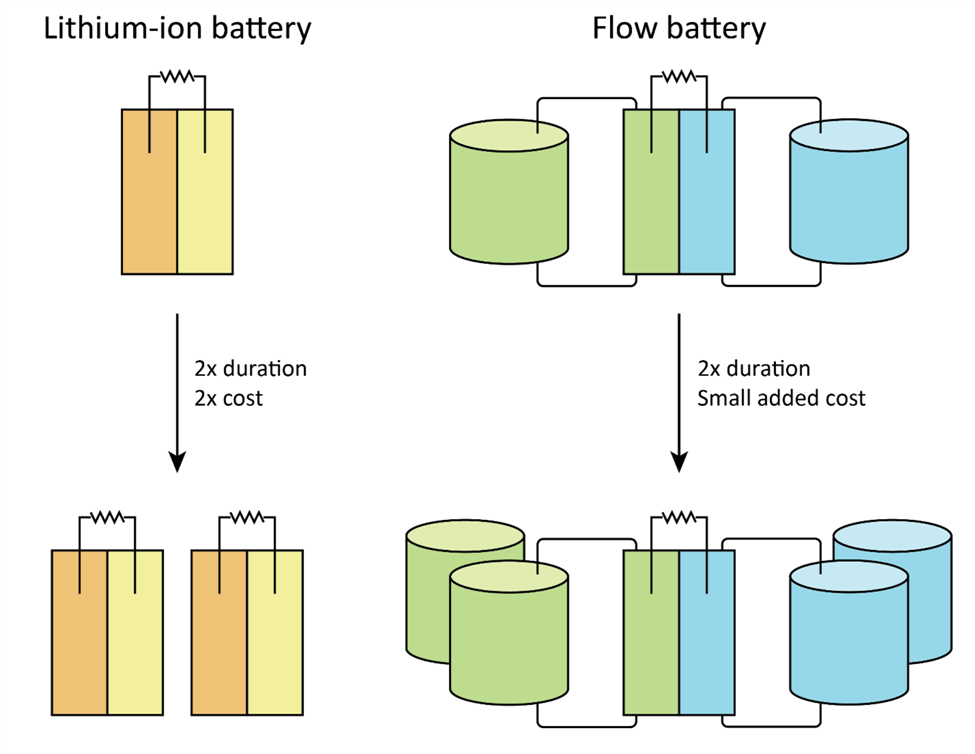
\includegraphics{fig/flow_battery.png}

In theory, flow batteries can scale up to almost any size, relatively cheaply. So as the demands for storage get bigger --- six hours, eight hours, 12 hours --- the economics of flow batteries look better and better relative to LIBs.

A variety of different metals can be used in the electrolyte. For a long while, vanadium was expected to be the breakout candidate, but materials costs remain stubbornly high. Companies have tried with zinc (like the late \href{https://www.greentechmedia.com/articles/read/distressed-vizn-seeks-lifeline-following-staff-layoffs}{ViZn}, and also see below) and iron (like ESS, which is still going strong). Recent history is \href{https://www.greentechmedia.com/articles/read/flow-batteries-struggle-in-2019-as-lithium-ion-marches-on}{littered with failed flow battery companies}.

Flow batteries have been the next big thing for a really long time.
The problem, as ever, is the steady march of LIBs down the cost curve.
For a three-or four-hour system, a lithium ion battery outperforms any flow battery now.
Flow batteries can theoretically expand their energy capacity indefinitely, for little more than the cost of the electrolyte goop to fill the tanks (though pumps and other accoutrement add to the cost a bit).
When we're below \$100 per kilowatt-hour on the cost of {[}LIBs{]} we are really close to the cost of the goop.

Flow batteries aren't going to be able to catch up to LIBs, at least not any time soon.

\href{https://www.volts.wtf/p/battery-week-competitors-to-lithium}{Volts}

\emph{CanaryMedia}

Instead of storing clean electricity in lithium-ion batteries, ESS makes a ``flow battery'' that moves electrons with a liquid mixture of iron and salt. ESS stands to capitalize on a few trends in the clean energy market:

Ten-year-old ESS announced in May that it would go public by merging with a special-purpose acquisition company (SPAC), a recently popular alternative to a traditional initial public offering.
ESS will be traded on the New York Stock Exchange with a valuation north of \$1 billion and the ticker symbol GWH.
It already has a factory pumping out flow batteries just south of Portland, Oregon.
The company built out the factory with a \$30 million Series C raise in 2019, led by SoftBank's SB Energy and Bill Gates--backed Breakthrough Energy Ventures.
the factory will be able to produce more than 1.5 gigawatt-hours of storage capacity annually.

Technicians take the pieces from the robots, compile them and load them into cargo boxes docked along the wall of the factory. After hooking up pipes and electronics and loading the tank with the dry powdered version of the iron liquid, a truck carries away the finished Energy Warehouse.

Leveraging cheaper materials than its competitors.
Conventional batteries become overly pricey when scaled up for many hours of storage; all ESS needs to do is add more rusty water to the tank, which makes the incremental cost of additional storage much smaller.

ESS is it's a relatively simple technology when it comes to flow batteries.''

In contrast, vanadium flow batteries, a perennial contender in the lithium-ion challenger category, suffer when vanadium prices skyrocket, as they have in recent years.

Flow-battery technologies that utilize low-cost redox species such as iron will have a cost advantage over vanadium.

One known challenge with iron flow batteries is hydrogen generation at the negative electrode that eventually leads to cell failure.
A commercial iron flow battery will either prevent the generation or mitigate it somehow.
ESS dealt with that by inventing what it calls a Proton Pump, which connects to the tank and passively mixes the unwanted hydrogen back into the solution. That maintains the balance of pH and states of charge in the liquid electrolyte circulating through the system.
That invention is a key commercial differentiator for ESS.
Other flow chemistries need to cease operations regularly to rebalance their electrolytes.

Another general hangup for flow batteries is the cost of membranes or separators that allow electrons to pass but keep other materials from mixing. But ESS uses off-the-shelf separators from the battery industry.

Then there's the worry that a system that pumps liquid for decades eventually will leak.
In the latest product iteration, ESS reduced the number of pipe connections per Energy Warehouse from 170 to 36. Instead of relying on threaded pipe connections that need to be tightened just right, the new pipes get ``thermally fused,'' which means they are melted together.

And for winning over customers to the technology itself, ESS points to an unusual program hammered out with German reinsurance giant Munich Re. That firm studied the technology and decided to offer a performance warranty, which covers costs if the technology doesn't perform as promised.
``Munich Re helps address the technology risk for the first few score buyers.

\href{https://www.canarymedia.com/articles/ess-is-betting-the-world-is-ready-for-a-billion-dollar-battery-disrupter/}{CanaryMedia}

\hypertarget{zinc}{%
\section{Zinc}\label{zinc}}

Batteries that exchange zinc ions instead of lithium ions --- it's the second-most-popular metal for batteries.

Zinc has the particular advantage of being light and energy dense like lithium, so with relatively modest adjustments, it can slipstream into the lithium-ion manufacturing process.

Zinc is plentiful, cheaper than lithium, largely benign, and makes batteries that are easier to recycle. Like other lithium alternatives, zinc sacrifices energy density, but makes some of it back up in savings on safety systems at the battery-pack level, thanks to the lack of any need for fire suppression. This puts it in the same markets as LFP: smaller commuter/city vehicles, robo-taxies, scooters, e-bikes --- and energy storage.

Some in the zinc crew have larger designs: ``We think we can coexist with lithium-ion and replace lead acid,'' says Michael Burz, president and CEO of EnZinc, which has developed a new zinc anode it says can come close to LIBs on energy density. Remember, lead-acid batteries are still ubiquitous. ``Forklifts use them. Airplanes. Snowmobiles.`` says Burz. ``Data centers have huge banks of lead-acid batteries they use for switchover power.'' It's still a \$45 billion global market.

EnZinc thinks it can hit a sweet spot: close to the energy density of LIBs, close to the low cost of lead-acid, safer than either, and good enough to substitute for a big chunk of both.

Zinc anodes are ``cathode agnostic,'' so Burz envisions, rather than becoming a battery manufacturer, becoming an anode supplier --- ``Zinc Inside,'' modeled on ``Intel Inside'' processors. Research is underway on a number of cathodes, from manganese and nickel to, just as with lithium, air. A zinc-air battery ``has a system-level specific energy of anywhere between 250 to 350 watt-hours per kilogram,'' says Burz, well above most LIBs. The trick is making it controllable and rechargeable.

Most of these batteries make the same basic claims: they are less energy dense than LIBs, but they are safer (no fires), they are made with benign and plentiful materials (no supply problems), and they are cheaper at high capacities/durations. It's just that last part that's tricky, since the price and capabilities of LIBs are a moving target.

\hypertarget{sodium-ion}{%
\section{Sodium-ion}\label{sodium-ion}}

Lithium, nickel, and cobalt all have their issues. You know what material doesn't? Salt.

Sodium compounds can be substituted for lithium compounds to create sodium-ion batteries (NIBs), which have been the source of considerable hype for at least five years now. The basic idea and manufacturing process is the same for NIBs as LIBs --- ``you could use existing gigafactory structures to produce a sodium-ion battery,'' says Steingart --- but unlike the latter, the former can't use graphite for the anode, because it can't capture enough of the relatively bigger sodium ions, so something called ``hard carbon'' is typically used instead.

Research is underway to find more energy-dense sodium compounds for the cathode and cheaper materials for the anode. ``Sodium-ion has a lower energy density than lithium-ion,'' says Tim Gretjak, an innovation analyst with Con Edison, ``so all the materials that go into it have to be correspondingly that much cheaper.''

\href{https://www.volts.wtf/p/battery-week-competitors-to-lithium}{Volts}

\hypertarget{liquid-metal}{%
\section{Liquid-Metal}\label{liquid-metal}}

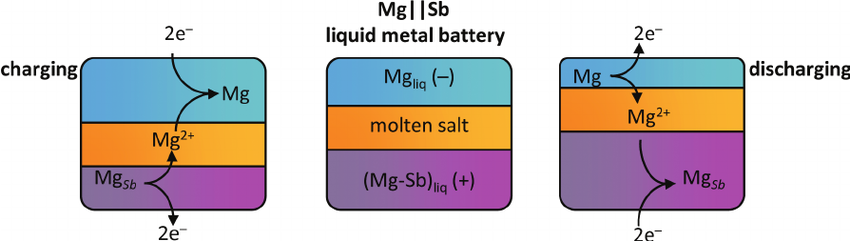
\includegraphics{fig/liquid_metal_battery.png}

The battery will pass no current at room temperature, but on site, the contents of the boxes are super-heated (to 500°C), which activates the materials; the metals alloy and de-alloy, with the cathode being entirely consumed and then reformed, as the batteries charge and discharge.

Because the contents are liquids, the battery has no ``memory'' --- it is not affected or degraded by absorbing or releasing ions. This means it suffers virtually no loss of capacity over its lifetime; in fact, it works better if completely charged and discharged every few days.

From the time they are first activated, liquid metal batteries require no outside heating or cooling for the lifetime of the system, eliminating a ton of system costs, and they can operate in a wide range of temperatures and conditions.

The batteries contain materials less than half the cost of LIB materials, can be manufactured for less than half the cost of LIBs, and will run for 20 years at a ``fraction of the cost'' of LIBs.

\href{https://www.volts.wtf/p/battery-week-competitors-to-lithium}{Volts}

\hypertarget{quantumscape}{%
\section{QuantumScape}\label{quantumscape}}

\emph{Wesoff}

QuantumScape claims to have solved the solid-state battery riddle that has stumped generations of battery scientists. It has created a commercially viable, rechargeable lithium metal battery with enough oomph to make it a contender to displace the internal combustion engine.

With potential energy density exceeding 400 watt-hours per kilogram, solid-state battery deployment could mark the tipping point for adoption of electric vehicles and open up massive transportation markets. QuantumScape's battery employs lithium metal anodes (referred to by the company as ``solid state''), which could be the key to the next wave of EV battery performance gains, according to the findings from BMW shown in the chart below.

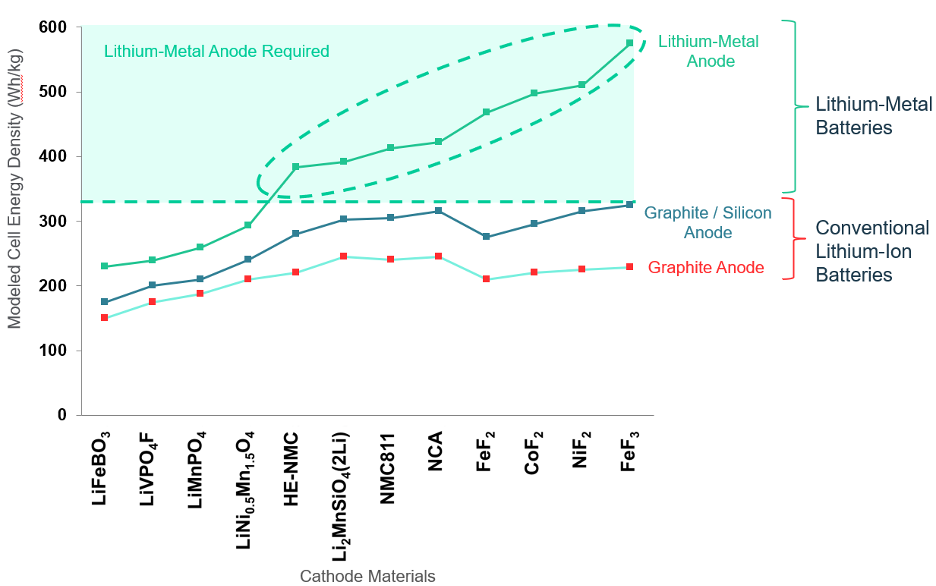
\includegraphics{fig/cathode-anode-materials-chart.png}

Among its many innovations, QuantumScape has replaced the polymer separator used in conventional lithium-ion batteries with a ceramic separator, enabling the use of an anode of metallic lithium instead of one made of carbon or carbon-silicon. The metallic lithium anode is formed in situ when the finished cell is charged.

A viable lithium-metal anode would allow higher energy density than is possible with conventional anodes and therefore longer driving range with the potential of faster charging, long cycle life and improved safety -- qualities that are fundamental to changing the minds of those reluctant to purchase an EV.

\begin{quote}
``I believe that retail investors and perhaps even the technical staff at Volkswagen have been severely underestimating the scale of the challenges facing QuantumScape. Manufacturing defect-free ceramic separators at meters-per-second speed is very unlike other manufacturing challenges faced by the battery or PV industry previously. This is insanely hard. Elon Musk always pounds his chest about''production hell" and how difficult making cars is. Making these ceramic separators will be at least 10× harder than any technical challenge Tesla {[}has{]} faced."
\end{quote}

A business parallel with solar that the storage industry might want to avoid is how the photovoltaic market coalesced around a narrow set of Chinese-made silicon technologies after a U.S. venture capital frenzy that set the solar investment clock back a decade. Manufacturability, cost reduction and actual industrial policy won the solar market for China, rather than exotic science.

QuantumScape is still a development-stage startup facing enormous technology and scaling risk as it attempts to move from lab to production.

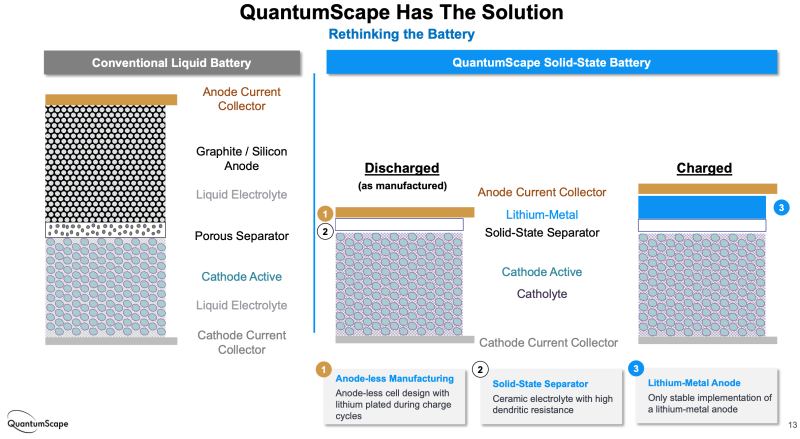
\includegraphics{fig/quantumscape.png}

\href{https://www.canarymedia.com/articles/quantumscapes-billion-dollar-battery-experiment/}{Wesoff}

\textbf{Quantumscape Scam?}

SPAC's are free to promote absurd financial projections and
timelines that are illegal in a typical IPO. The current SPAC
mania is partly fueled by insiders exploiting this loophole to
lure retail investors, setting them up as bagholders for the
pump and dump, when the lockup expires and they cash in.
We think QS is a textbook case.

\href{pdf/Scorpion_2021_Quantumscape.pdf}{Scorpion (2021) QuantumScape SPAC Scam (pdf)}

Massive investments in lithium-ion (Li-ion) battery manufacturing capacity,
which is expected to more than triple to 1.3 TWh by 2023.

Li-ion batteries' scaling pathway is unlike that for silicon
photovoltaic cells; investment continues to differentiate
among chemistries with performance attributes that are
best suited to specific use cases.

Solid-state technology is poised to massively disrupt
the storage industry by unlocking new opportunities for
cheap, safe, and high-performing batteries.

Meeting electricity goals for \textless2C° global temperature increase
may require deploying batteries much faster than Li-ion price decreases
are predicted to enable (unless demand flexibility can be increased).

High renewable penetration modeling scenarios generally assume that
3\%--7\% of the total installed renewable capacity is required as additional
interday energy storage to account for forecast and demand uncertainty.

If 60\% of the 6,500 GW of current global electricity generation capacity
were met with variable renewable energy, it would require between 120
and 280 GW of long duration storage, or enough capacity to power France
plus Germany.

\href{pdf/rmi_breakthrough_batteries.pdf}{RMI Breakthrough Batteries (pdf)}

65;6203;1c
\# Energy Storage

\emph{Wesoff}

The potential is great and the grid surely needs it, but long-duration energy storage still has a long way to go.

Long-duration storage can accelerate the retirement of peaker plants, defer upgrades of transmission and distribution infrastructure, and improve the dispatchability of renewables such as solar and wind -- theoretically, at least.

Systems with more than 100 hours of energy storage capacity provide the most benefit to the grid.

Long-duration storage can reduce the costs of deeply decarbonized electricity systems by 10 percent if the storage technology's costs are below \$20/kilowatt-hour. The savings could reach as high as 40 percent if long-duration storage costs could be reduced to \$1/kilowatt-hour.

Economic long-duration energy storage doesn't exist. Yet.

Today's high-growth, gigawatt-scale energy storage market is absolutely dominated by lithium-ion batteries with short durations ranging from minutes to a few hours and used largely in ancillary, not energy, applications.

\hypertarget{pumped-hydro}{%
\section{Pumped Hydro}\label{pumped-hydro}}

Pumped storage (which consists of pumping water from a low reservoir to a higher-elevation reservoir, and then releasing that water to spin turbines and generate power) accounts for 95\% of all utility-scale energy storage in the U.S.

America's 43 pumped storage plants were mostly built between 1960 and 1990 to support nuclear power and have a total combined capacity of roughly 100 gigawatts of storage. There are a number of new plants in development that are being built, in this case, to help support renewables rather than nuclear.

The problems with new pumped hydro projects: "They cost billions of dollars and take years to build, and can run afoul of environmental opposition

\textbf{New Design}

On Oregon's Klamath River, a coalition of Indigenous groups, environmental advocates and other stakeholders will soon remove four hydropower dams erected between 1903 and 1962. The goal is to revitalize the ecosystem --- and the surrounding economy.

Upriver and roughly 10 miles northeast of Klamath Falls, as the crow flies, Rye Development hopes to build a new type of hydropower plant altogether.

The Swan Lake Energy Storage Project would have no connection to surrounding rivers. Rye plans to excavate two 60-acre holes and fill them with water it has already secured. The water would cycle up and down the closed system as the plant charges and discharges electricity.

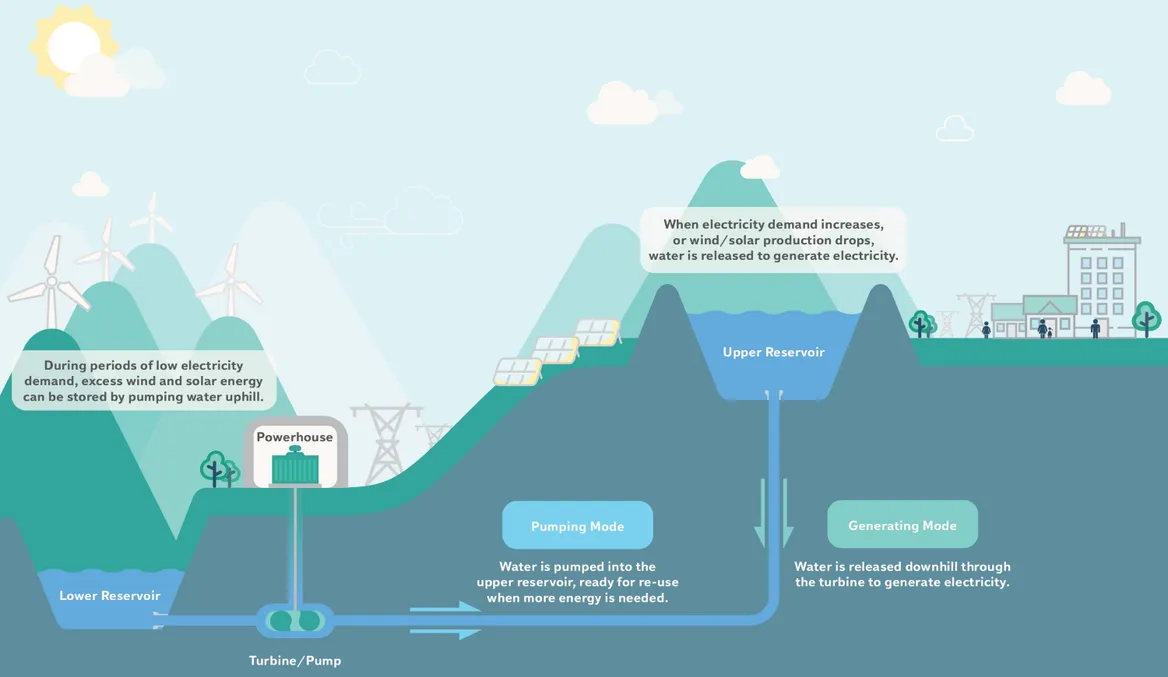
\includegraphics{fig/pumped_hydro.png}

Two ponds may not seem radical, but they mark a decisive break with the past.

\href{https://www.canarymedia.com/articles/long-duration-energy-storage/pumped-hydro-grid-storage-could-be-poised-for-a-comeback}{Canary Media (2022) Pumped Hydro Come-back}

\hypertarget{flow-batteries-1}{%
\section{Flow Batteries}\label{flow-batteries-1}}

Flow batteries circulate a liquid electrolyte through stacks of electrochemical cells and have long held the promise of 10-hour durations, tens of thousands of cycles, minimal degradation and no limitations on depth of discharge. This performance promise has lured venture capital investment and research and development --- but so far, the investments have yielded few commercial, competitive flow battery products.

\hypertarget{mechnical-energy-storage}{%
\section{Mechnical Energy Storage}\label{mechnical-energy-storage}}

Compressed-air energy storage remains a contender. The Los Angeles Department of Water and Power selected Range Energy and Mitsubishi Power Systems to develop underground salt caverns to store high pressure air (or someday hydrogen)

Raise a rail car, a huge weight and a water column, respectively, with low-cost or curtailed energy, generating power when the mass is lowered.

Quidnet will use excess renewable energy to store pressurized water underground in dry oil and gas wells.

\emph{HydroStor}

Construction entails digging large-diameter shafts underground, one of which will be filled with water from aboveground tanks. Compressors on the surface will push air into the cavern, where it presses against the column of water to maintain a steady pressure. When released, that compressed air will spin 100-megawatt turbines that regenerate power. All that construction work is expected to take three to four years.

\href{https://www.canarymedia.com/articles/hydrostor-is-developing-truly-massive-grid-storage-in-watery-caverns/}{Canary Hydrostor}

\hypertarget{thermal-storage}{%
\section{Thermal Storage}\label{thermal-storage}}

Thermal storage uses excess or curtailed power to charge a thermal ``battery'' made of materials such as molten salt or cryogenic liquids.

\emph{HeatCrete}

Norway-headquartered EnergyNest makes its own branded ThermalBattery product which essentially stores heat in a patented form of concrete, which it has dubbed Heatcrete. A heat transfer fluid (HTF) at high temperatures passes through steel pipes cast into the `battery', in technology that the company claims enables storage of energy at very low CapEx cost, using low-cost materials in a simple design. EnergyNest has previously said the Heatcrete materials can last 30 to 50 years of use without degradation.

\href{https://energy-nest.com/}{EnergyNest}

\href{https://www.energy-storage.news/news/thermal-energy-storage-startup-energynest-secures-us130-million-investment?utm_source=newsletter\&utm_medium=email\&utm_campaign=canary}{CanaryMedia}

\hypertarget{software-market-flex}{%
\section{Software (Market Flex)}\label{software-market-flex}}

Lee Kasten, a WECC-based power system operator, suggests that we should rely on software and markets, not hardware: ``Where possible, we should use software over hardware. For example, don't build a battery that costs a billion dollars, only works 2\% of the time and only moves around 100 {[}gigawatt-hours{]} of electricity. Build an energy-imbalance market or an extended day-ahead market for \$50 million or \$100 million that moves around hundreds of gigawatts of electricity. Give all consumers price signals, and then watch the flexible consumers adapt to those price signals using software to manage existing loads.''

\href{https://www.canarymedia.com/articles/long-duration-storage-roundup-news-players-and-technology/}{Wesoff (canary Media)}

\hypertarget{compressed-air}{%
\section{Compressed Air}\label{compressed-air}}

\emph{Canary Media}

Hydrostor stores surplus electricity by compressing air into underground caverns. It updates a long-standing technology that never took off for electrical storage. Hydrostor thinks the tweaks it has made will allow underground storage to work in more places --- just as grids increasingly need help turning wind and solar production into reliable 24/7 electricity.

Goldman Sachs agreed and invested \$250 million from its private equity division. That's unusual for the long-duration energy storage sector, which typically draws riskier venture-capital investment.

To build these projects, Hydrostor excavates an 8-foot-diameter shaft that goes 2,000 feet deep. Workers descend to hollow out a cavity, which the company then floods. When it's time to \hspace{0pt}``charge,'' the aboveground facility compresses air and shoots it below the water barrier. To discharge, it releases the compressed air, which spins a turbine and produces electricity.

These projects are designed for eight hours of discharge at full power capacity. But the technology can provide longer storage durations with a bigger cavern to hold more air.

``All we need is reasonably competent bedrock.''

\href{https://www.canarymedia.com/articles/long-duration-energy-storage/goldman-sachs-just-made-a-record-setting-investment-in-long-duration-energy-storage}{Canary Media (2022) Hydrostor}

\hypertarget{amoniac}{%
\chapter{Amoniac}\label{amoniac}}

\emph{TU}

Spillvarme har en hovedrolle

Fordi ren ammoniakk brenner dårlig og er vanskelig å tenne, er ideen til forskerne å bruke spillvarmen fra forbrenningsprosessen til delvis å spalte ammoniakken. Ammoniakk består av ett nitrogenatom og tre hydrogenatomer. Etter spaltingen sitter vi igjen med drivstoff som består av ammoniakk, nitrogen og hydrogen.

Hydrogenandelen i dette brenselet bidrar med å sparke forbrenningsprosessen godt i gang, med god hjelp fra store mengder med oppvarmet luft fra omgivelsene. Det gir bevegelse og framdrift i motorens velkjente termiske prosess.

At «arbeidsmediet» i denne forbrenningen er luft, gjør det ganske enkelt og billig å skalere opp prosessen, sånn at den kan tilpasses de største cargoskipene. For batteridrevne skip eller fartøy som bruker kraft fra brenselceller, er det en god del vanskeligere, sier Gruber.

Muligheten for oppskalering gjør at løsningen er perfekt for store skip -- som i dag ofte drives av forurensende tungolje.

\href{https://www.tu.no/artikler/ammoniakk-kan-gjore-langdistanse-skipsfart-helgronn/511245}{TU}

\hypertarget{bio-fuel}{%
\chapter{Bio Fuel}\label{bio-fuel}}

\emph{Beslik}

Biomass is defined as any plant matter used directly as fuel or converted into other forms before combustion. Included are wood, vegetal waste (including wood waste and crops used for energy production), animal materials/wastes, sulphite lyes (also known as ``black liquor'') and other solid biomass. The word biofuel is usually reserved for liquid or gaseous fuels, used for transportation.

Currently biomass covers approximately 10 percent of the global energy supply, of which two-thirds is used in developing countries for cooking and heating.

Biomass currently represents almost 60\% of the EU's renewable energy, more than solar and wind power combined, according to the EU's statistical office, Eurostat.

In the EU, Germany is the leading producer of solid biomass. Production volumes reached an estimated 12.8 million metric tons of oil equivalent, which was 2.6 million metric tons more than France, ranked second. Total primary energy production in the EU amounted to 96.9 million metric tons in 2019.

One of the biggest problems related to large scale biomass supply is the energy density that is needed to decarbonise heavy CO2 emitting industries.

Last year, a group of climate activists filed a lawsuit against the EU to challenge the notion that forest biomass is carbon neutral, a principle which is currently enshrined in the bloc's renewable energy directive.

According to this group ``the treatment of biomass as carbon neutral runs counter to scientific findings'' which shows that burning wood for energy typically emits 1.5 times more CO2 than coal and 3 times more than natural gas, the plaintiffs claimed.

The European Court of Justice dismissed the case, saying the activists had failed to demonstrate how the directive was of ``individual concern'' to them. Which is by all means almost funny.

Like fossil fuels, biomass releases carbon dioxide emissions upon combustion. While there is an argument for carbon balancing -- due to the carbon dioxide that is removed from the atmosphere by trees and plants during their lifetimes via photosynthesis -- these are nevertheless emissions that could be avoided if other renewable sources like wind or solar were used instead.

In addition to CO2, burning biomass fuels results in the release of various other harmful gases such as carbon monoxide, NOx (nitrogen oxides), and VOCs (volatile organic compounds), which all contribute to air pollution.

Providing the feedstocks used in biomass power plants -- frequently in the form of wood pellets -- requires large areas of forest and woodland to be cut down. Proponents will argue that all trees are replaced with new ones, that can grow, remove carbon, and be used for future energy needs.

But this cycle requires strict adherence to sustainable land management and responsible agriculture throughout the supply chain. And as biomass power stations grow in number, demand for these materials will multiply accordingly -- exerting greater pressure on a natural resource that is already under threat from other industries.

There are biodiversity considerations too, because while an area of forest might be replaced to grow anew over time, the wildlife and ecosystems that are displaced by these actions are faced with a more immediate challenge that is not solved by planting young trees.

\href{https://esgonasunday.substack.com/p/week-18-is-biomass-an-energy-source}{Beslik}

\emph{Swiss voting}

A majority of Swiss voters also backed a free trade deal with Indonesia, which would expand palm oil imports at lower tariffs. Indonesia, a world away, is the site of a vast ecocide, destroying tropical forests (which are also carbon sinks) on an immense scale, driving countless species, including the Orang Utan, extinct, to make way for palm oil plantations. The palm oil goes to us consumers in the West. Roughly half of palm oil ends up burned in our cars as biodiesel, thanks to European Union rules aiming to replace fossil fuels with bio-based fuels. This rule arguably kick-started the ecocide in Indonesia --- the clear result of problem shifting (from climate disaster to biodiversity calamity, although in fact the climate benefits of bioenergy are extremely dubious) rather than tackling the root cause: unsustainable overconsumption. The other half of palm oil ends up in food and cosmetics, and can easily be substituted with other, slightly more expensive, ingredients.

In this case, a majority of the Swiss people voted, in full knowledge, to continue to participate in ecocide and exploitation, far across the world, for cheaper access to various goods including palm oil, and for preferential terms for Swiss firms in Indonesia. They decided that a few economic advantages in consumption and production were worth it: they made the calculus, and decided that ecocide was worth it. It's one thing when your government or business leaders decide that ecocide is worth it to gain economic advantage. It's something else entirely to be walking around the streets of a country where a majority of the people you meet and greet made the ghastly calculation to be complicit in ecocide for a few more francs.

A few months ago, a majority of the Swiss population voted differently, but in vain. They voted to curb multinational corporations, and hold them accountable for human rights violations (including environmental damage) overseas. Sadly, this majority was not sufficient: a majority of cantons (regions) was also necessary, and this fell woefully short. A majority of people in the rural cantons, the places upheld as the heartland of traditional Swiss values by the far-right, voted to continue to allow multinational corporations based in Switzerland to violate human rights and degrade the environment overseas with complete impunity. Again, a few more Swiss francs are worth more than child labour or poisoning local populations. Nice values, eh?

\href{https://jksteinberger.medium.com/the-bear-the-tiger-and-the-trade-unionist-4b25df5fb3a9}{Steinberger}

\hypertarget{fuel-cells}{%
\chapter{Fuel Cells}\label{fuel-cells}}

Fuel cells are scaling up exactly as solar and wind did in previous decades.

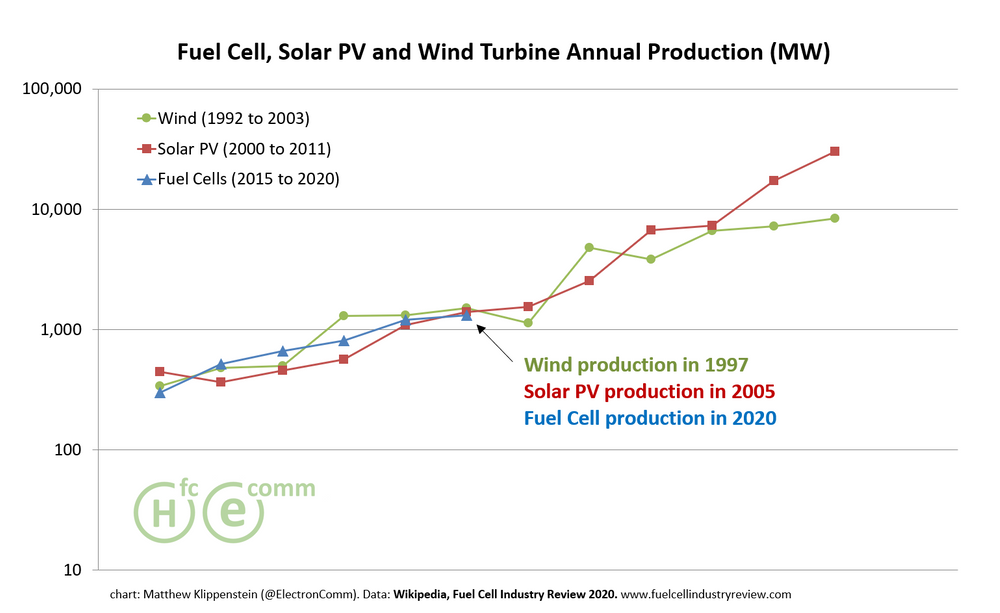
\includegraphics{fig/fuel-cell_catch-up.png}

Fuel cells electrochemically convert hydrogen and oxygen into direct-current electricity.

Fuel cells employ an assortment of electrolytes, catalysts and temperatures. But in almost all cases, the membranes are expensive to fabricate, and the technologies require precious metal catalysts (typically platinum or palladium) or high process temperatures. Input fuels range from natural gas to methanol to hydrogen. Ongoing research and development efforts, some led by the DOE, are underway to reduce the need for expensive metals and to improve the reliability and lifetime of the fuel cell stack.

Common technologies include proton-exchange membrane (PEM), solid oxide (SOFC), phosphoric acid (PAFC) and molten carbonate (MCFC). There are a number of other technologies, all adept at destroying investor capital. GE, GM, Hyundai, Honda, Johnson Matthey, Panasonic, Siemens, Samsung, LG, Sharp, Toshiba and Toyota have all invested in (and in many cases ultimately abandoned) fuel cell technology.

Bloom Energy, Doosan and FuelCell Energy build large stationary fuel cells, using SOFC, PAFC and MCFC technologies, respectively. Plug Power, on the other hand, targets its PEM fuel cell system at powering forklifts and other vehicles in the enormous materials handling market.

While Bloom's and FuelCell Energy's equipment runs on natural gas, Plug Power's PEM fuels cells run on pure ``five nines'' hydrogen and work most productively with a hydrogen infrastructure at the customer site.

The U.S. Department of Energy continues to fund fuel cell development, most recently with \$33 million to support hydrogen and fuel cell research and development, infrastructure supply-chain development and validation, and cost analysis activities.

\href{https://www.canarymedia.com/articles/chart-of-the-day-fuel-cell-industry-profits/}{Wesoff}

\hypertarget{geothermal}{%
\chapter{Geothermal}\label{geothermal}}

\begin{quote}
It is the only other thing that you could essentially attach to the current grid, almost anywhere in the world --- in fact, below current cities. It seems like science fiction, right? Drilling to the center of the earth? But it's not. It's a super exciting clean power generation area
\end{quote}


\includegraphics{fig/geothermal_US_10km.png}

\emph{Figure: U.S. geothermal resources at 10 kilometers depth}

\href{https://www.canarymedia.com/articles/hot-and-bothered-about-geothermal-energy/}{CanaryMedia}

\emph{Enthalpy}

Enthalpy is a property of a thermodynamic system, defined as
the sum of the system's internal energy and the product of its pressure and volume,
H = U + pV.
It is a convenient state function standardly used in many measurements
in chemical, biological, and physical systems at a constant pressure.
The pressure-volume term expresses the work required to establish the system's physical dimensions,
i.e.~to make room for it by displacing its surroundings.
As a state function, enthalpy depends only on
the final configuration of internal energy, pressure, and volume,
not on the path taken to achieve it.

The unit of measurement for enthalpy in the International System of Units (SI) is the joule.
Other historical conventional units still in use include the British thermal unit (BTU) and the calorie.

The total enthalpy of a system cannot be measured directly because the internal energy contains components that are unknown, not easily accessible, or are not of interest in thermodynamics. In practice, a change in enthalpy (ΔH) is the preferred expression for measurements at constant pressure, because it simplifies the description of energy transfer. When matter transfer into or out of the system is also prevented, the enthalpy change equals the energy exchanged with the environment by heat.

\href{https://en.wikipedia.org/wiki/Enthalpy}{Enthalpy - Wikipedia}

\hypertarget{heat-storage}{%
\section{Heat Storage}\label{heat-storage}}

\emph{Low Enthalpy Aquifer Technology}

\href{https://rudenas.com/}{Ruden Energy}

\hypertarget{deep-drilling}{%
\section{Deep Drilling}\label{deep-drilling}}

\hypertarget{ultra-deep-drilling}{%
\subsection{Ultra Deep Drilling}\label{ultra-deep-drilling}}

Quaise Energy Inc.~has teamed with the Laboratory for Scientific Computing (LabSC) to develop computational models of the interaction of high-energy beams with geological materials.
The models developed will provide understanding of the fundamental physics underlying the operation of a gyrotron-powered millimeter-wave (MMW) energy drilling system developed by Quaise, a spin-off company born from research at MIT (Massachusetts Institute of Technology) Plasma Science and Fusion Center.

This new, breakthrough technology will be used for MMW drilling to reach depths of 10-20 km below the earth's surface, which is beyond what can be accomplished today using conventional drilling.
Deep drilling will enable harvesting supercritical geothermal energy with power densities several order of magnitudes larger than wind or solar energy, thus opening the opportunity for accessing a clean, carbon-free and power-dense energy source anywhere around the world.

The successful development of a commercial system has to overcome technical challenges related to the interaction of millimeter electromagnetic waves with basement rock formations at extreme conditions and far-field transport of material.

\href{https://www.thinkgeoenergy.com/research-partnership-to-explore-ultra-deep-geothermal-drilling/}{Think Geoenergy (News)}

\emph{Canary Media on Quaise}

The earlier experiments at MIT produced 10-centimeter-deep holes in palm-sized slabs of rock. At Oak Ridge, Quaise has vaporized 3-foot-deep holes into larger rocks using the national lab's more powerful megawatt-size gyrotrons. This year, the startup is planning to drill about 30 feet into the actual ground outside the Oak Ridge facility.

The company is planning to drill a 330-foot well in New Mexico or Colorado with the oil-and-gas drilling contractor Nabors Industries, which invested \$12 million in the startup last year.

After that, Quaise could drill a 3,300-foot-deep hole near the Newberry Volcano in Bend, Oregon. AltaRock, which is studying the crater, has called the site \hspace{0pt}``probably the biggest untapped geothermal resource in North America.'' Geologists believe a shallow magma body sits only 6,500 to 16,500 feet below the surface. Drilling here would allow Quaise to validate its technology in supremely hot conditions without having to dig too far down to start.

If Quaise succeeds in demonstrating its novel approach, the startup plans to drill ultra-deep wells not just on the sides of volcanoes but primarily alongside existing power plants.

Instead of coal or natural gas, steam produced with the earth's heat could drive turbines and generate electricity using existing infrastructure. Power plants tend to be built near population centers, reducing the need for the long transmission lines that connect remote wind and solar farms. And existing plants tend to sit atop private property, which could potentially help Quaise avoid legal challenges like those facing geothermal projects on public land.

Among the biggest risks for any advanced drilling system is seismic activity. In recent years, geothermal projects using different types of technologies were shut down in Switzerland, South Korea and France after triggering earthquakes and rattling surrounding cities.

\href{https://www.canarymedia.com/articles/geothermal/geothermal-startup-quaise-raises-40m-for-ultra-deep-drilling}{Canary Mediaon Quaise (2022)}

\emph{North Sea Geothermal}

Platforms in the UK North Sea could be converted to run on geothermal energy, providing power to the offshore field facilities or feeding power to markets in Europe via trans-North Sea interconnector grids.

Traditionally, once an oil or gas field reaches the end of its productive life, its production platform is decommissioned. The structure may be removed and taken ashore for recycling/reuse, or part of the platform may remain on the seabed, perhaps creating an artificial reef. However, another alternative is becoming a more viable option -- re-using the platform to extract geothermal energy. If applied to redundant platforms in the North Sea, this could create a whole new industry employing thousands of workers in new productive jobs in the offshore and onshore support sectors.


\includegraphics{fig/North_Sea_UK_geothermal.png}

Figure: UK 50 hottest geothermal gradient wells by degrees C.

The UK continental shelf (UKCS) where many platforms are situated has a relatively thin earth's crust -- around 10 km (6.2 mi) thick compared to 40-70 km (25-43 mi) thick on land -- which gives the wells their high bottomhole temperatures. There are more than 50 wells in the region with a geothermal gradient more than 122°F (50°C)/km, the highest being 296°F (147°C)/km. At Total's Elgin-Franklin high-pressure/high-temperature (HP/HT) gas condensate development in the UK central North Sea, one of the wells was drilled to a depth of 6,100 m (20,013 ft), with a temperature of 387°F (197°C) and a pressure of 16,750 psi (1,155 bar).

Heat from these wells could be employed to generate electricity on board the platform that could in turn be routed to the UK's national grid via subsea cables. North Sea platforms have the advantage of being surrounded by cold sea water, which is at a much lower temperature than the onshore air cooling towers that are the conventional means of condensing a generating plant's working fluids after they have passed through the turbines.

It would also be possible to re-inject waste heat remaining in the fluids back into the subsurface oil-bearing level to increase field pressure and flows, thereby enhancing secondary oil recovery and extending field life. Furthermore, discovery of further oil fields might follow when drilling to greater depths to tap the geothermal energy beneath the platforms.

Geothermal energy has huge potential when set in context against other energy reserves. All fossil fuels, i.e.~coal, oil and gas, come from the earth's crust. The crust makes up only 0.4\% of the total mass of the planet, the remaining 99.6\% being hotter than 932°F (500°C) within the crust, increasing to 9,032°F (5,000°C) at the core. The pressures within the earth are constantly generating this heat naturally. This means that geothermal energy is infinite in its nature, as it is naturally renewable.

Recent research carried out in Russia, in the Kola Peninsula, has revealed moving fluids and open fractures at depths more than 12 km (7.5 mi). This discovery has led to a review of current deep geological thinking and has opened the development of geothermal energy extraction for electrical power generation.

There are three types of geothermal energy. One -- Geo-pressure -- is where you have a high wellhead pressure, to which you can attach a hydroelectric type turbine to generate the power or electrical power from a natural gas letdown station. The twin screw turbine design from Langson Energy produces 1 MW electrical output, operating in temperatures from 350-550°F (177-288°C) and up to pressures of 600 psi (42 bar). This is already deployed by the natural gas industry to generate power, where the gas mains changes pressure to use the power instead of it being wasted. A second is created by separating the gas from the oil/water brine and using it like a diesel-type generator, i.e.~burning the gas to produce power, which could provide an alternative to flaring on certain offshore installations. The third involves using the temperature, as in the high-pressure steam, steam, Organic Rankine Cycleturbine system. This approach could be applied to platforms or on a nearby support vessel.

\href{https://www.offshore-mag.com/pipelines/article/16762144/geothermal-power-an-alternate-role-for-redundant-north-sea-platforms}{Offshore Magazin}

\hypertarget{drilling-technology}{%
\subsection{Drilling Technology}\label{drilling-technology}}

\emph{Løberg (facebook `Geotermisk Elektrisitet' 210123)}

Ny brønnteknologi for geotermisk elproduksjon under utvikling. \#regjeringen \#enova I dag utvikles det meget raske og fleksible boreløsninger, f.eks en vanntrykk-hammer som ikke trenger borestreng, en kompakt drillbit under vanntrykk som borer i stål og fast fjell, som kan brushe opp casinger som er klogget, det er utviklet plasmaboresystemer som kan nå store dyp og høye temperaturer. Closed loops i gamle brønner kan bruke f.eks CO2 som arbeidsgass, og med temperatur og trykk på 4500 meter kan gassen bli superkritisk, slik at den kan trekke til seg store mengder varme. Det er kjent kunnskap (CO2 har vært brukt i kjøleskap etc i 20-30 år). Det er gjort prototyper som har testet CO2 i lukkede sløyfer/closed loops, og det er gjort beregninger på potensialet. Det er flere selskaper som spesialiserer seg på closed loop-systemer. Norge er faktisk med på dette også, som på Island, Indonesia etc. Vi kan gjøre det på Svalbard, og fase ut vårt kullkraftverk, som nå skal gå på diesel som er fraktet dit med skip. Hva med naturgass i mellomtiden, før det fases over til geotermisk el og varme?

Det finnes mye info på våre sider om dette. Skal vi få geotermisk el og varme opp i bevisstheten, må vi sette oss inn i elementene jeg har nevnt i denne posten. Bare studer linkene under og del med de som bør oppdatere seg:

\href{https://www.tu.no/artikler/den-norske-oppfinneren-har-en-visjon-om-at-kinesiske-kullkraftverk-kan-bygges-om-til-geotermiske-kraftverk/376346}{Hammergy, norsk utviklet boreteknologi}

\href{https://techxplore.com/news/2022-01-micro-drilling-turbines-efficiency-geothermal.html}{Drillbit} utviklet av Fraunhofer IEG i Bochum og Fraunhofer-Chalmers Research Center for Industrial Mathematics FCC i Sverige.

\href{pdf/high_macpherson_ht_directional_drilling.pdf}{High-Temp 330C Drilling System (pdf)}

\href{https://www.euractiv.com/section/energy/opinion/european-technology-unlocking-deep-geothermal-energy-for-all/}{Plasmakutting} kan brukes ned til 10 000 meter med temperaturer på 300-400 grader.

\href{https://www.journals.elsevier.com/renewable-energy-focus}{Drilling/smelting med millimeter-bølger}

\href{pdf/Liu_2017_Drilling_Water_Jet.pdf}{Roterende vannjet Liu (2017) (pdf)}

Closed loop selskap, \href{https://www.euractiv.com/section/energy/news/closed-loop-technology-brings-promise-of-geothermal-anywhere/}{EAVOR}

\href{https://www.greenfireenergy.com/how-does-geothermal-energy-work/}{Gjenbruk av en brønn med closed loop og CO2}

Les rapporten \href{pdf/Almaya_2020_Closed_Loop_geothermal.pdf}{her (pdf)}

Se en informativ film \href{https://youtu.be/g0sHVsC1cF4}{her}
Lær om ulike \href{https://youtu.be/PtQmGPmyLA0}{geotermiske systemer og closed loop}

\hypertarget{nevada}{%
\section{Nevada}\label{nevada}}

\emph{CanaryMedia}

Fervo, which raised a \$28 million Series B round in April, aims to make geothermal more competitive by applying advanced drilling technologies from the oil and gas industry. Horizontal drilling and underground fiber-optic sensors already make oil and gas drilling more efficient, but they can reduce costs and increase productivity for geothermal as well.

Small modular nuclear reactors require years of regulatory vetting before they can be built. Long-duration energy storage needs to be tested, at small scales and usually for years, before customers will trust it. But advanced geothermal doesn't involve any radically different technology, so its path to market could be swifter.
Geothermal doesn't have to reinvent the wheel.

The partnership with Google extends beyond power delivery and into data crunching as well. Fervo will work with Google's cloud analytics and artificial intelligence capabilities to study the data collected while drilling. One objective is to understand how to optimize geothermal plants as flexible resources,

Geothermal currently supplies just 0.4 percent of U.S. electricity.
But a \href{https://www.energy.gov/sites/default/files/2019/06/f63/GeoVision-full-report-opt.pdf}{Department of Energy study} suggests this 24/7 renewable resource could reach as much as 120 gigawatts installed by 2050, delivering 16 percent of the country's electricity, if technological improvements take hold and gain traction.

\href{https://www.canarymedia.com/articles/google-taps-geothermal-for-corporate-clean-energy/}{CanaryMedia}

\hypertarget{china}{%
\section{China}\label{china}}

\emph{Smelror (in Norwegian)}

I gjennomsnitt øker temperaturen nedover i dypet med rundt 3° C for hver 100 m.
Geologiske variasjoner som varmeproduksjon og termisk konduktivitet kommer først inn som en viktig faktor ved 1000 m og dypere. Her vil varmeproduksjon fra nedbryting av radioaktivt materiale ha mye å si for den geotermiske gradienten.

Geotermisk energi i dag ikke dekker mer enn 1 \% verdens totale behov for energi.
10 av de 15 landene med høyest andel geotermisk energi utviklingsland (inkludert El Salvador, Guatemala, El Salvador, Filippinene og Kenya).

Et av de landene som satser sterkest på å utnytte geotermisk energi er Kina. Målet er å produsere 560 000 GWh elektrisitet innen 2015. Selv om dette ikke vil dekke mer enn 1,7 \% av landets totale energiforbruk, vil dette tilsvare et forbruk på 68,8 millioner tonn standard kullekvivalenter. Det er beregnet av bruken av grunn geotermisk energi i de 287 største byene vil kunne tilsvare en produksjon på 2,8 millioner GWh elektrisk strøm. Fratrukket nødvendig strømbruk til utvikling og drift av varmepumpene, vil dette tilsvare et forbruk på 250 millioner tonn kullekvivalenter, noe som igjen vil tilsvare 500 millioner tonn redusert utslipp av karbondioksid. I tillegg vil Kina produsere geotermisk energi fra 12 ulike områder med varme kilder, tilsvarende et forbruk på 4,52 millioner tonn kullekvivalenter, tilsvarende et redusert utslipp av karbondioksid på hele 1,3 milliarder tonn.

Potensialet blir ennå mer overveldende hvis man også tar i betraktning muligheten for utnyttelse av dyp geotermisk energi på en regional skala også utenfor de 12 høytemperatur-områdene. Dette vil kreve en storstilt satsning på energibrønner boret ned til mellom 3000 m og 10 000 m. I følge nyere beregninger kan man få ut energi tilsvarende 860 trillioner tonn kullekvivalenter, noe som tilsvarer mer enn 7 trillioner GWh elektrisk strøm, og som er nok til å dekke Kinas totale årlige energiforbruk 260 000 ganger.

For å kunne utnytte potensialet for geotermisk energi må det framskaffes ny geologisk kunnskap. Vi må kjenne til løsmassemektigheter, ha kunnskap om hydrogeologiske forhold i undergrunnen, kjenne til porøsitet og permeabilitet i reservoarene dypt nede i undergrunnen, vi må kjenne til varmeproduksjon og varmeledningsevne i de ulike bergartene, og vi må vite hvor store rom i undergrunnen de geotermiske reservoarene strekker seg over. Bærekraftig energi for alle handler mye om geologi. De som ønsker å gjøre en forskjell ved å bidra til en verden med økt bruk av miljøvennlige energikilder, gjør klokt i å velge en utdanning som gjør at de kan omsette gode intensjoner til konkret handling. I så måte er kunnskap innen geologi et godt og nødvendig fundament.

\href{https://www.geoforskning.no/blogg/item/baerekraftig-energi-for-alle}{Smelror}

\hypertarget{us}{%
\section{US}\label{us}}

In this paper, we identify the technological, economic, and political reasons that the United States has failed to exploit its geothermal resources. We provide actionable policy recommendations to sustainably and economically utilize the vast energy reserves under our feet.

\href{https://inn\%20ovationfrontier.org/geothermal-everywhere-a-new-path-for-american-renewable-energy-leade\%20rship/}{Geothermal Everywhere: A New Path for American Renewable Energy Leadership}

\hypertarget{hydro-power}{%
\chapter{Hydro Power}\label{hydro-power}}

Today the technical potential for hydropower development around the world is much greater than the actual production: the percent of potential hydropower capacity that has not been developed is 71\% in Europe, 75\% in North America, 79\% in South America, 95\% in Africa, 95\% in the Middle East, and 82\% in Asia-Pacific.

This is significant if you think about transition we need to make.

Due to the political realities of new reservoirs in western countries, economic limitations in the third world and the lack of a transmission system in undeveloped areas, perhaps 25\% of the remaining technically exploitable potential can be developed before 2050, with the bulk of that being in the Asia-Pacific area.

Some countries have already developed their hydropower potential and have very little room for growth: Switzerland for example produces 88\% of its potential and Mexico 80\%.

Today we have around 1,300 GW of installed hydropower capacity globally. According to the International Renewable Energy Agency (IRENA)'s \href{https://www.irena.org/-/media/Files/IRENA/Agency/Publication/2020/Apr/IRENA_Global_Renewables_Outlook_2020.pdf}{Global Renewables Outlook 2020}, this figure will need to grow by around 60 per cent by 2050 to help limit the rise in global temperature to well below 2 degrees Celsius above pre-industrial levels.

While a large hydropower facility can often provide low-cost electricity for 50 to 100 years after being built, the upfront construction costs can be large. This, combined with the fact that suitable places for reservoirs are becoming rarer over time, means that large-scale hydropower plant construction costs may continue to rise.

A \href{https://phys.org/news/2020-05-exploring-impacts-climate-hydropower-production.html}{study by researchers from IIASA and China} investigated the impacts of different levels of global warming on hydropower potential and found that this type of electricity generation benefits more from a 1.5°C than a 2°C climate scenario.

Environmental concerns about dams typically centre on their blockage of fish migrations or their upstream impacts, such as the inundation of habitats and the displacement of human communities. However, dams can cause serious downstream impacts as well. Although the public generally thinks of threats to aquatic organisms solely in terms of water quality, hydrological alteration -- the modification of downstream water flow regimes caused by dams and infrastructure -- is one of the primary causes of the degradation of freshwater ecosystems worldwide.

Unfortunately, hydropower's global track record of managing environmental and social impacts and assuring equitable distribution of social benefits has been less than stellar. So the occasional generality thrown out by the most vigorous proponents, that hydro is `environmentally friendly', rings hollow and calls for a more careful analysis.

No hydropower project is likely to be 100\% sustainable. All projects must be viewed as more or less sustainable.

To address the environmental and social concerns and guide the pursuit of sustainability, several entities have developed policies that articulate `sustainable hydro power', including Green Hydro in Switzerland and the Low Impact Hydropower Institute in the US, in addition to the guidance on sustainability presented in the World Commission on Dams report.

Recently, the International Hydropower Association (IHA) has developed both sustainability guidelines and a sustainability assessment protocol. Collectively, these documents describe specific measures for hydropower planning and operation that can be used to evaluate the sustainability of a hydro project or programme.

\href{https://esgonasunday.substack.com/p/week-17-why-is-no-one-talking-about}{Beslik}

\hypertarget{hydrogen}{%
\chapter{Hydrogen}\label{hydrogen}}

\hypertarget{home-hydrogen}{%
\section{Home Hydrogen}\label{home-hydrogen}}

\emph{Guardian}

In the remote hills of Cumbria, a few miles north of Hadrian's wall, three nondescript terrace houses stand side by side, quietly offering a glimpse of a low-carbon future.

The houses are intentionally unremarkable in every way but one: they are the first in the UK to run on a blend of clean-burning hydrogen as part of the most sophisticated hydrogen testing facility in the world. Welcome to Hystreet.

Engineers at the five-hectare site are testing whether hydrogen can safely replace the fossil-fuel gas pumped through transmission pipes and local grid networks into British homes as part of the government's efforts to meet climate targets.

``Ninety-nine percent of people don't think about where their gas comes from, or how it gets there,'' says Antony Green, National Grid's hydrogen tsar and head of the FutureGrid project. His task is to create a realistic replica of the UK's gas system to test whether the same pipelines that have carried gas from the North Sea into homes since the 1970s could transport low-carbon hydrogen in the future.

Heating British homes accounts for 15\% of the country's total emissions, meaning a low-carbon alternative will be crucial to cut emissions to net zero by 2050. But the testing site is also key to understanding how hydrogen can be transported to major factories and industrial clusters to help tackle emissions from polluting factories and power plants.

``The evidence we have built over the last few years shows that we can do this,'' Green says, walking along the length of a giant gas pipe. ``It's all very well and good doing the paperwork. But you still need to prove it.''

Using the UK's existing gas infrastructure to carry hydrogen is no simple task. It is more combustible than the traditional methane-rich gas we have learned to use safely in our homes, and its smaller molecules mean it is three times more likely to leak from pipelines or into homes than fossil gas. On the plus side, hydrogen is also lighter, meaning it is more likely to dissipate than to pool and create a combustion threat.

Like natural gas, hydrogen is odourless, so would have the same distinctive smell added to help people quickly notice a leak. When it burns, it is hard to see in daylight, so the hob has an adjustment that produces a visible flame, similar to that of a traditional gas hob but redder in colour.

For the sceptics, the challenge of overhauling the UK's 4,000 miles of underground gas pipelines is too costly a step when heating and cooking could run on a low-carbon electricity system instead.

The opposing factions in the debate run along predictable industry lines. National Grid and other companies that operate legacy gas infrastructure or gas production projects tend to favour home hydrogen, to prolong the life of existing assets. Energy companies that invest in low-carbon electricity generation tend to back electric heat pumps as the future for low-carbon homes.

\emph{Blue Hydrogen}

Although blue hydrogen is widely considered ``low-carbon'', it has failed to win favour among climate campaigners. Despite using carbon-capture technology to trap emissions from the process, about 10\% to 15\% of the CO2 in the fossil gas would find its way to the atmosphere. It would also require continuing offshore gas production, which carries a hefty carbon footprint.

\href{https://www.theguardian.com/environment/2021/oct/30/hydrogen-high-street-could-these-homes-change-the-way-we-keep-warm}{Guardian}

\hypertarget{green-vs-blue-hdrogen}{%
\section{Green vs Blue Hdrogen}\label{green-vs-blue-hdrogen}}

\emph{Longdon Abstract}

Hydrogen produced using fossil fuel feedstocks causes greenhouse gas (GHG) emissions, even when carbon capture and storage (CCS) is used. By contrast, hydrogen produced using electrolysis and zero-emissions electricity does not create GHG emissions. Several countries advocating the use of `clean' hydrogen put both technologies in the same category. Recent studies and strategies have compared these technologies, typically assuming high carbon capture rates, but have not assessed the impact of fugitive emissions and lower capture rates on total emissions and costs. We find that emissions from gas or coal based hydrogen production systems could be substantial even with CCS, and the cost of CCS is higher than often assumed. Carbon avoidance costs for high capture rates are notable. Carbon prices of \$22--46/tCO2e would be required to make hydrogen from fossil fuels with CCS competitive with hydrogen produced from fossil fuels without CCS. At the same time there are indications that electrolysis with renewable energy could become cheaper than fossil fuel with CCS options, possibly in the near-term future. Establishing hydrogen supply chains on the basis of fossil fuels, as many national strategies foresee, may be incompatible with decarbonisation objectives and raise the risk of stranded assets.

\emph{Longdon Highlights}

• Emissions from gas or coal based hydrogen systems are substantial even with CCS.
• Fugitive emissions are rarely included in national and international H2 strategies.
• CCS is an expensive option for decarbonising hydrogen production.
• Electrolysis with renewable energy could become cheaper than fossil fuels with CCS.

\href{https://www.sciencedirect.com/science/article/abs/pii/S0306261921014215}{Longdon (2021) `Clean' hydrogen? -- Comparing the emissions and costs of fossil fuel versus renewable electricity based hydrogen (paywall)}

\emph{Guardian}

Green hydrogen beats blue on emissions and financial cost.

{[}Guradian (2021) \url{https://www.theguardian.com/australia-news/2021/nov/18/green-hydrogen-beats-blue-on-emissions-and-financial-cost-australian-study-finds})

\hypertarget{wind-to-hydrogen}{%
\section{Wind to Hydrogen}\label{wind-to-hydrogen}}

Siemens Gamesa and Siemens Energy have announced plans to invest €120m (\$146m)
in a five-year strategy to unlock the potential of
harvesting green hydrogen from offshore windpower.

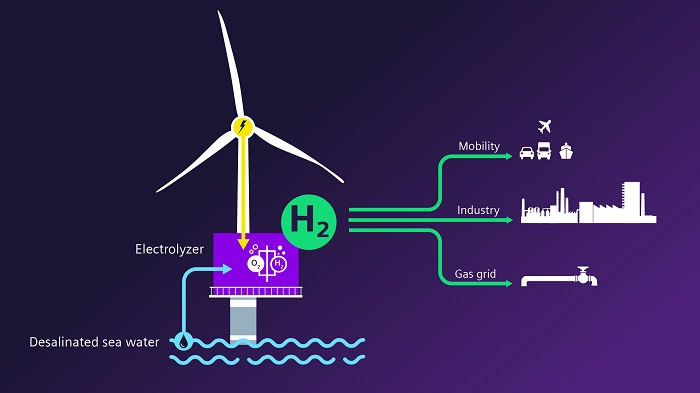
\includegraphics{fig/Hydrogen_Offshore-Electrolysis_Siemens.jpg}

The companies are collaborating on a solution to integrate
an electrolyzer into an offshore wind turbine
as a single synchronized system to directly produce green hydrogen.

\hypertarget{hydrogen-aviation}{%
\section{Hydrogen Aviation}\label{hydrogen-aviation}}

\emph{Heynes}

In 2008, Boeing flew the first hydrogen-powered aircraft whilst ZeroAvia flew the world's first hydrogen-powered commercial aircraft in 2020. But the main industry player, already in the works to present hydrogen-powered aircraft to the market, is Airbus.

For hydrogen-powered aircraft, hydrogen can be used in two ways: as a fuel source for fuel cells, when hydrogen reacts with oxygen to produce electricity that powers the engine or alternatively it can be used directly as a fuel source in a modified engine.

Airbus is looking at both these methods for aircraft with the company presenting three models of modified aircraft that would be operated using hydrogen and has already committed to have the first aircraft in service by 2035.

Because hydrogen can be extracted from water, airports could generate their own hydrogen fuel, reducing the need for fuel transportation, eliminating related emissions and possible transportation safety hazards.

The potential of hydrogen as aviation fuel is undeniable, but there is still a long way to go. The constantly growing attention to aviation sustainability will act as a catalyst in making a hydrogen-powered aircraft a reality.

Revolutionary hydrogen technology for aviation and urban air mobility has been unveiled today (2nd March) by HyPoint -- and the Californian fuel cell specialist is expecting to start shipping the product in 2022.

HyPoint says its NASA award-winning turbo air-cooled hydrogen fuel cell system will cut years off commercial delivery timelines for hydrogen aircrafts and unlock the emerging hydrogen aviation market.

The company claims its technology delivers an unprecedented combination of specific power and energy density and has passed key validation testing to prove its technical viability.

\href{https://www.h2-view.com/story/hydrogen-aviation-projected-to-be-worth-174bn-by-2040/}{Heynes}

\hypertarget{nuclear}{%
\chapter{Nuclear}\label{nuclear}}

\emph{Beslik}

The nuclear dilemma.

Nuclear power is dead. Long live nuclear power. Nuclear power is the only way forward. Nuclear power is too dangerous. Nuclear power is the safest power source around. Nuclear is nothing. Nuclear is everything.

When I started looking at this I was stunned by how the same numbers and indicators can be interpreted in so fundamentally different ways.

The same basic data set -- nuclear plants currently in existence, those under construction, the status of new technologies, the history of costs and delays, and a few striking accidents -- produces totally contradictory opinions and predictions.

Nuclear power is a Rorschach test: You see what you want to see, a rosy nuclear future or an old-world dinosaur in a slow-death spiral. It's a reflection of your own views on the energy present and future.

In all likelihood, no one will be proven right or wrong for decades.

The state of nuclear power

Nuclear power today accounts for around 10 percent of the total electricity generation around the world.

This varies sharply by country. In the U.S. the rate is about 20 percent, in Russia and Germany it is a bit lower than that, while some other European countries get 40 and 50 percent from nuclear reactors.

France has long led the way proportionally, at more than 70 percent (it has the second most total reactors, behind the U.S.). China, though building rapidly, drew less than 3 percent of its power from nuclear in 2014.

There are 442 reactors currently in operation globally, and the International Atomic Energy Agency says that 66 are currently under construction. Twenty-four of those are in China; no other country is currently building more than eight.

Read more \href{https://world-nuclear.org/information-library/current-and-future-generation/nuclear-power-in-the-world-today.aspx}{here}

and \href{https://world-nuclear.org/information-library/nuclear-fuel-cycle/introduction/nuclear-fuel-cycle-overview.aspx}{here}.

In general, the more experience accumulated with a given technology, the less it costs to build. This has been dramatically illustrated with the falling costs of wind and solar power.

Nuclear, however has bucked the trend, instead demonstrating a sort of ``negative learning curve'' over time.

The nuclear industry's main hope for future expansion lies in a new generation of small modular reactors (SMRs) that generate less than 300 MW each and are amenable to assembly-line construction.

These are still under development, however, with none licensed or under construction.

In the U.S. nuclear power generates as much as \$50 billion each year from electricity sales and revenue, and provides around 100,000 jobs.

A handful of companies and governments are working to develop small-scale nuclear reactors (SMRs) that proponents say are safer, cheaper, and more compatible with renewables than traditional nuclear power.

But critics contend the new technology doesn't address concerns about safety and radioactive waste.

Small modular reactors suffer from many of the same problems as large reactors, most notably safety issues and the unresolved problem of what to do with long-lived radioactive waste. And opponents say that even in a smaller form, nuclear power is expensive --- it's one of the costliest forms of energy, requiring substantial government subsidies to build and run, not to mention insure.

In 80-odd years of nuclear power, in which more than 450 commercial reactors, many experimental stations and tens of thousands of nuclear warheads have been built, great stockpiles of different levels of waste have accumulated.

About 0.2--3\% by volume is high-level waste.
Mostly derived from civil reactor fuel, this is some of the most dangerous material known on Earth, remaining radioactive for tens of thousands of years. It requires cooling and shielding indefinitely and contains 95\% of the radioactivity related to nuclear power generation.

Further 7\% or so by volume, known as intermediate waste, is made up of things like reactor components and graphite from reactor cores. This is also highly dangerous, but it can be stored in special canisters because it does not generate much heat.

Around 22,000 cubic meters of solid high-level waste has accumulated in temporary storage but not been disposed of (moved to permanent storage) in 14 western countries, along with unknown amounts in China, Russia and at military stations.

A further 460,000 cubic meters of intermediate waste is being stored, and about 3.5 million cubic meters of low-level waste.

Some 34,000 cubic meters of new high-level and intermediate waste is generated each year by operating civil reactors,

The bitter reality is that there is no scientifically proven way of disposing of the existential problem of high- and intermediate-level waste.
The truth is that whatever efforts are made to bury and forget it, it will not go away.

Nuclear stands for 10\% of world energy supply.

\href{https://esgonasunday.substack.com/p/week-16-is-nuclear-part-of-our-sustainable}{Beslik}

\hypertarget{fukushima}{%
\section{Fukushima}\label{fukushima}}

\textbf{Release of radioactive waste into sea}

Japan has announced it will release more than 1m tonnes of contaminated water from the wrecked Fukushima nuclear power plant into the sea, a decision that has angered neighbouring countries, including China, and local fishers.

Official confirmation of the move, which came more than a decade after the nuclear disaster, will deal a further blow to the fishing industry in Fukushima, which has opposed the measure for years.

The prime minister, Yoshihide Suga, told a meeting of ministers on Tuesday that the government had decided that releasing the water into the Pacific Ocean was the ``most realistic'' option, and ``unavoidable in order to achieve Fukushima's recovery''.

The plant's operator, Tokyo Electric Power {[}Tepco{]}, and government officials say tritium, a radioactive material that is not harmful in small amounts, cannot be removed from the water, but other radionuclides can be reduced to levels allowed for release.

China denounced the plan as ``extremely irresponsible'', and accused Japan of reaching the decision ``without regard for domestic and foreign doubts and opposition''.

``This approach is extremely irresponsible and will seriously damage international public health and safety and the vital interests of the people of neighbouring countries,'' the Chinese foreign ministry said in a statement on its website.

South Korea summoned Japan's ambassador, Koichi Aiboshi, the broadcaster YTN reported, while a high-level government official said Seoul ``firmly opposes'' the move, a view also expressed by Taiwan's Atomic Energy Council.

The US was supportive, describing Japan's decision-making process as ``transparent''.

The announcement drew swift condemnation from environmental groups.

About 1.25m tonnes of water has accumulated at the site.
It includes water used to cool the plant, as well as rain and groundwater that seeps in daily.The radioactive water, which increases in quantity by about 140 tonnes a day, is now being stored in more than 1,000 tanks, and space at the site is expected to run out around next autumn.

The International Atomic Energy Agency supports the decision, since radioactive elements, except tritium, will be removed from the water or reduced to safe levels before it is discharged. The IAEA has also pointed out that nuclear plants around the world use a similar process to dispose of wastewater.

Experts say tritium is only harmful to humans in large doses and with dilution the treated water poses no scientifically detectable risk.

Local fishing communities say the water's release will undo years of hard work to rebuild consumer confidence in their seafood.

Japanese officials have objected to media descriptions of the water as ``contaminated'' or ``radioactive'', insisting that it be described as ``treated''.

Shaun Burnie, senior nuclear specialist with Greenpeace East Asia, said that claim was ``clearly false''.
``If it was not contaminated or radioactive they would not need approval (to release the water) from Japan's nuclear regulator,'' he said. ``The water in the tanks is indeed treated, but it is also contaminated with radioactivity. The Japanese government has been deliberately seeking to deceive over this issue, at home and abroad.''

\href{https://www.theguardian.com/environment/2021/apr/13/fukushima-japan-to-start-dumping-contaminated-water-pacific-ocean}{Guardian (210413)}

\hypertarget{james-hansens-position}{%
\section{James Hansen's Position}\label{james-hansens-position}}

\emph{James Hansen obviously thinks climate cannot be saved without nuclear power}

Development and deployment of 4 th generation nuclear power to
the point that modular nuclear reactors provide electricity cheaper than coal. By 4 th generation I
refer to all modern passively-safe reactors, whether thorium or uranium fueled -- even nuclear
fusion, which at long last is now closer than 50 years away.

The preposterous fear of nuclear waste from power plants --
which is held in containers where it harms nobody -- is hyped, while poorly-contained waste
from other energies is ignored. Waste from heavily-subsidized fossil fuels is spewed in the air
freely. About 20,000 people per day die of outdoor and indoor air pollution -- much of that
pollution being waste from fossil fuel combustion. People drop like flies from that pollution --
more than are killed by pandemics and wars combined -- but politicians pay little heed.

Even 2 nd generation nuclear power
plants can be operated safely. The one serious accident in the U.S. -- at Three-Mile Island --
caused no deaths. Modern nuclear reactors that shut down in case of an anomaly and cool the
nuclear fuel without need for external power are our safest energy. Neither the Chernobyl nor
Fukushima accidents would have occurred with modern nuclear power.

Passive safety features are available that allow reactor shutdown and cooling without external
power or operator intervention.

{[}James Hansen: Planet.Chapter47{]}

\hypertarget{fusion---iter}{%
\section{Fusion - ITER}\label{fusion---iter}}

ITER was set in motion at the Geneva Superpower Summit in November 1985, when the idea of a collaborative international project to develop fusion energy for peaceful purposes was proposed by General Secretary Gorbachev of the former Soviet Union to US President Ronald Reagan.

The People's Republic of China and the Republic of Korea joined the Project in 2003, followed by India in 2005. Selecting a location for ITER was a lengthy procedure that was concluded in 2005, when the ITER Members unanimously agreed on the site proposed by the European Union. The ITER installation would be built near Aix-en-Provence in southern France.

More than 200 tokamaks around the world have paved the way to the ITER experiment.

Conceived as the last experimental step to prove the feasibility of fusion as a large-scale and carbon-free source of energy, ITER will be the world's largest tokamak, with ten times the plasma volume of the largest tokamak operating today.

\href{https://www.iter.org/proj/iterhistory}{ITER}

\hypertarget{thorium}{%
\section{Thorium}\label{thorium}}

\emph{Tekna Energibloggen}

Norge har atter engang trukket vinnerloddet! Vi sitter på nok thorium til å erstatte all norsk energiproduksjon i over 2000 år. Dette er også en teknologi som kan kutte alle utslipp fra store skip og kutte kostnadene samtidig. Norge kan således også ta igjen vårt tapte marked innen deep-sea og større skip, generelt. Mulighetene er enorme, men det kommer ikke av seg selv.

\textbf{Saltsmeltereaktorer}

Foredraget handler blant annet om en teknologi innen kjernekraft -- saltsmeltereaktorer -- som ble først utviklet på 1960-tallet men lagt i skuffen under den kalde krigen da teknologien ikke produserte materialer for våpen. Dette skjedde til tross for at det amerikanske kjernekraftkommisjonen anså dette som en meget lovende teknologi, og 3 år med feilfri drift av en prototype bekreftet dette -- den har faktisk ingen av de risikoelementene vi tradisjonelt forbinder med kjernekraft. Teknologien er også mye billigere enn tradisjonelle kjernekraftverk og den er mye enklere å skalere fra smått til stort. Dessverre ble teknologien ansett for å ikke ha noen sikkerhetspolitisk betydning og lagt i skuffen, men etter 9/11 ble denne teknologien tatt frem fra støvet igjen av samme grunn -- trygghet og ikke-spredning. I dag er teknologien en av de mest innovative teknologiene som finnes innen energiområdet. Dette er reaktorer som kan bygges så små som 1 MW men også så store som 3.000 MW, og blant de 67 forskjellige små reaktordesignene som nå utvikles, er saltsmeltereaktorer en av de mest interessante. Det er fordi saltsmeltereaktorer kan løse verdens utslippsproblematikk svært kostnadseffektivt med forventet kostnadsnivå på kun 25 øre/kWh, der er ingen risikoelementer som man tradisjonelt forbinder med kjernekraft, og den har lave investeringskostnader.

\href{https://www.tekna.no/fag-og-nettverk/energi/energibloggen/thorium-og-saltsmeltereaktorer/}{Tekna (2021) Thorium og saltsmeltereaktorer}

\hypertarget{melted-salt-reactors}{%
\section{Melted Salt Reactors}\label{melted-salt-reactors}}

\emph{Seaborg}

I utgangspunktet vil Seaborg bruke et uranbrensel som kalles HALEU -- High-assay low-enriched uranium. Det inneholder mellom 5 og 20 prosent U235.

Vi vil blande uranet med fluor og lage urantetrafluorid, som vi så blander med andre salter basert på Na og Ka. De vil senke smeltepunktet til rundt 500 grader. Den høye berikningen av U235 er kostbar, men vi slipper å bruke brenselstaver, som er veldig kostbart.

På grunn av den høye temperaturen i det smeltede saltet kan reaktorene produsere en variabel kombinasjon av strøm og varme eller produsere hydrogen.

Det er i selve reaktoren at atomreaksjonen finner sted og varmen genereres. Den hentes ut via varmeveksling til nok en saltkrets som ikke inneholder radioaktive stoffer. Så varmeveksles den videre til en vannkrets med 200 bars trykk som produserer damp til en turbin som driver en generator. Alternativt kan energien tas ut som varme, eller noe midt imellom.

Når reaktoren er fylt med det radioaktive saltet, vil den kunne gå kontinuerlig i tolv år uten tilførsel av mer saltbrensel. Da er det meste av det fissile materialet brukt opp, og resten vil være resirkulerbart. Det vil si at det kan gjenbrukes i en annen reaktor slik at mer energi kan hentes ut. Avfallets behov for lagringstid blir redusert til 300 år. I forhold til det som skal lagres, er det veldig små volumer sammenlignet med energien som produseres. Og den raske halveringstiden gjør lagringen enklere.

Sammenlignet med tradisjonelle reaktorer er Seaborgs anlegg mye enklere, og de slipper kravene til kompliserte sikkerhetssystemer som driver opp prisen på konvensjonelle kjernekraftverk.

I stedet for å bruke grafitt som moderator, bruker vi natriumhydroksid.
Reaktoren har en driftstemperatur på i underkant av 600 grader. Det er ideelt til dampproduksjon og gjør at de kan bruke standard dampturbiner. Hvis reaktoren skal produsere hydrogen, blir det veldig effektivt mellom 800 og 900 grader.

Selve reaktorkjernen er utformet som en sylinder med en diameter på to meter og høyde to meter. Når den er i drift må alt som inneholder oksygen holdes utenfor reaktoren.

Den flytende steinen som saltet i praksis er, krever høy temperatur for å være flytende. Skulle noe skje, vil det stivne under 490 grader. Reaktoren kan ikke smelte ned eller eksplodere eller lekke radioaktive gasser til luft eller vann. Og teknologien kan ikke brukes for å lage våpen.

Når saltet er flytende, er det også mulig å benytte såkalte ispropper, det vil si et materiale med høyere smeltepunkt. Skulle reaktortemperaturen blir for høy, vil proppen smelte og saltet renne ut i flere beholdere hvor kjernereaksjonene stopper.

Seaborg vil installere reaktorene på båter eller flåter.
Det er plass til mellom to og åtte reaktorer i en flåte, hver reaktor er på 100 MW. På grunn av monteringen på flåter kan leveringstiden reduseres til tre år.

\href{https://www.tu.no/artikler/seaborg-utvikler-mobile-kjernekraftverk/516722}{Teknisk Ukeblad (2022)}

\hypertarget{oil}{%
\chapter{Oil}\label{oil}}

The global oil and gas industry consumes 3-4\% of global primary energy supply to extract,
transport, and refine energy products.

\hypertarget{carbon-intensity-of-crude-oil-production}{%
\section{Carbon Intensity of Crude Oil Production}\label{carbon-intensity-of-crude-oil-production}}

\emph{Mansadi Abstract}

The goals of the Paris Agreement pose challenges
to the oil and gas sector given the need to meet energy demand globally while limiting
greenhouse gas (GHG) emissions. We preliminarily quantify the heterogeneity of crude oil
well-to-refinery carbon intensities (CIs) by performing field-by-field life-cycle analysis
(LCA) of nearly 9,000 global oilfields representing \textasciitilde98\% of 2015 worldwide crude oil
production. The global volume-weighted average upstream CI estimate is 10.3 g
CO 2 eq./MJ crude oil, with country-level emissions ranging from 3.3 to 20.3 g CO 2 eq./MJ.
Gas flaring and thermal extraction of heavy crude oils are the two major drivers of high
GHG intensities. Global methane venting and fugitive emissions are poorly documented,
yet evidence suggests they can increase the CI estimates considerably. Upstream gas
management strategies alone could potentially mitigate \textasciitilde18 Gt CO 2 eq in the 21 st century.
Policy insights from this analysis regarding resource management, resource prioritization
and emerging technologies could enable a reduction in the GHG footprint from the oil and
gas industry.


\includegraphics{fig/carbon_intensity_of_crude_oil_production.png}

\href{https://www.osti.gov/pages/biblio/1485127}{Masnadi (2018) Global carbon intensity of crude oil production}
\href{pdf/Masnadi_2018_Carbon_Intensity_of_Crude_Oil_Production.pdf}{(pdf)}
\href{pdf/Masnadi_2018_Carbon_Intensity_of_Crude_Oil_Production_SM.pdf}{(pdf SM)}
\href{https://eao.stanford.edu/research-areas/opgeehttps://eao.stanford.edu/research-areas/opgee}{OPGEE Estimation Tool}

\hypertarget{renewable}{%
\chapter{Renewable}\label{renewable}}

Solar and wind potential is far higher than that of fossil fuels and can meet global energy demand many times over, unlocking huge benefits for society.

With current technology and in a subset of available locations we can capture at least 6,700 PWh p.a. from solar and wind, which is more than 100 times global energy demand.
Opportunities unlocked

The collapse in renewable costs in the last three years means that half of this solar and wind technical potential now has economic potential, and by the end of the decade it will be over 90\%.

The land required for solar panels alone to provide all global energy is 450,000 km2, 0.3\% of the global land area of 149 million km2. This differs by country as highlighted below.

\href{https://carbontracker.org/reports/the-skys-the-limit-solar-wind/}{carbonTracker}

\hypertarget{solar}{%
\chapter{Solar}\label{solar}}

\hypertarget{software-drives-solar-costs}{%
\section{Software drives Solar Costs}\label{software-drives-solar-costs}}

Software will eat solar: Driving utility-scale solar prices below 1 cent per kilowatt-hour by 2025

Terabase Energy is on a mission to get utility-scale solar power prices below \$0.01 per kWh by 2025 using software, as opposed to the DOE's hardware strategy.

Terabase Energy is on a mission to drive down utility-scale solar power prices to less than \$0.01 per kilowatt-hour by 2025, by using software, automation and modeling to optimize power-plant operation. The VC-funded startup just acquired another startup to help realize that goal.

Terabase's aggressive cost target far exceeds the U.S. DOE's SunShot 2030 goal of \$0.03 per kWh for utility-scale photovoltaics by 2025. The DOE's most recent solar funding went toward hardware improvements in nonsilicon solar approaches such as perovskites, cadmium-telluride thin films and next-generation concentrated solar power. The DOE target cuts the cost of solar energy by 60\% within the next 10 years.

But the 82\% reduction in solar cost over the last decade (according to the International Renewable Energy Agency) came from economies of scale, better technology and supply chains at largely silicon-based solar plants, not the alternative technologies being funded by the DOE.

And even silicon module pricing might be nearing the bottom of the cost curve: ``The era of ever-declining solar module prices is largely behind us,'' according to Yan Zhuang, president of Canadian Solar's manufacturing operation, as reported in pv magazine. Global commodities such as aluminum and glass are a larger part of the solar module bill of materials.
Software is eating solar

It's software, not hardware, that's going to drive down utility-scale solar costs, according to Terabase, a startup that closed a \$6 million Series A round late last year and has already made a small acquisition to further develop its platform. Terabase just acquired REPlant Solutions, a spinout of First Solar that makes solar power plant controls and has developed a 1.5-kilovolt direct-current (DC) architecture and a DC trunk bus.

REPlant's plant controller operates the solar power plant, acting as the ringmaster in an increasingly complicated process.

Matt Campbell, Terabase CEO, tells Canary Media: ``In the future\ldots PV plants will become even more demanding, requiring sophisticated plant controls, the integration of storage, and hybridization with wind and other forms of generation.'' The acquisition of REPlant adds advanced supervisory control and data acquisition (SCADA) and other controls systems to Terabase's toolbox.

REPlant has an installed base of more than 10 gigawatts across 80 solar plants.

\textbf{Big solar is more manufacturing than construction}

While solar hardware has gotten cheaper, soft costs are still stubborn and represent a more significant piece of the total project cost (a similar situation to the residential and commercial solar segments).

``We have to keep fighting to reduce the cost,'' said Campbell. ``There's a big difference between solar at 1 cent per kWh versus 1.5 cents per kWh.''

In an earlier interview, Campbell said that he wants to eliminate the construction mindset: ``Utility-scale solar is more manufacturing than construction, with tens of thousands of identical units. It's not complex like a dam. It's just big. {[}\ldots{]} It needs to be managed like row-crop farming and more of a modern, integrated supply chain. Most projects are still managed on Excel spreadsheets.''

The way to get to super-cheap solar, according to the CEO, is with smart software ``across the whole life cycle'' --- from procurement, to oversight of construction, to operations --- ``all on a common interconnected digital platform.''

Terabase recently provided digital and engineering services for the 800-megawatt Siraj-1 solar power plant in Qatar, which will sell its power for \$0.01449/kWh. (These low utility-scale solar cost numbers tend to happen in global markets with lower labor costs than the U.S.)

\href{https://www.canarymedia.com/articles/software-will-eat-solar-driving-utility-scale-solar-prices-below-1-cent-per-kilowatt-hour-by-2025/}{CanaryMedia: Software drives Solar}

\hypertarget{efficiency}{%
\section{Efficiency}\label{efficiency}}

\emph{Stevenson}

To make a really efficient device, it is tempting to pick a material that absorbs all the Sun's radiation -- from the high-energy rays in the ultraviolet, through to the visible, and out to the really long wavelengths in the infrared. That approach might lead you to build a cell out of a material like mercury telluride, which converts nearly all of the Sun's incoming photons into current-generating electrons. But there is an enormous price to pay: each photon absorbed by this material only produces a tiny amount of energy, which means that the power generated by the device would be pitiful.

A better tactic is to pick a semiconductor with an absorption profile that optimizes the trade-off between the energy generated by each captured photon and the fraction of sunlight absorbed by the cell. A material at this sweet spot is gallium arsenide (GaAs). Also used in smartphones to amplify radio-frequency signals and create laser-light for facial recognition, GaAs has long been one of the go-to materials for engineering high-efficiency solar cells. These cells are not perfect, however -- even after minimizing material defects that degrade performance, the best solar cells made from GaAs still struggle to reach efficiencies beyond 25\%.

Further gains come from stacking different semiconductors on top of one another, and carefully selecting a combination that efficiently harvests the Sun's output. This well-trodden path has seen solar-cell efficiencies climb over several decades, along with the number of light-absorbing layers. Both hit a new high last year when a team from the National Renewable Energy Laboratory (NREL) in Golden, Colorado, unveiled a device with a record-breaking efficiency of 47.1\% -- tantalizingly close to the 50\% milestone (Nature Energy 5 326). Until then, bragging rights had been held by structures with four absorbing layers, but the US researchers found that six is a ``natural sweet spot'', according to team leader John Geisz.

Getting this far has not been easy, because it is far from trivial to create layered structures from different materials. High-efficiency solar cells are formed by epitaxy, a process in which material is grown on a crystalline substrate, one atomic layer at a time. Such epitaxial growth can produce the high-quality crystal structures needed for an efficient solar cell, but only if the atomic spacing of each material within the stack is very similar. This condition, known as lattice matching, restricts the palette of suitable materials: silicon cannot be used, for example, because it is not blessed with a family of alloys with similar atomic spacing.

Devices with multiple materials -- referred to as multi-junction cells -- have traditionally been based on GaAs, the record-breaking material for a single-junction device. A common architecture is a triple-junction cell comprising three compound semiconductors: a low-energy indium gallium arsen­ide (InGaAs) sub-cell, a medium-energy sub-cell of GaAs and a high-energy sub-cell of indium gallium phosphide (InGaP). In these multi-junction cells, current flows perpendicularly through all the absorbing layers, which are joined in series. With this electrical configuration, the thickness of every sub-cell must be chosen so that all generate exactly the same current -- otherwise any excess flow of electrons would be wasted, reducing the overall efficiency.

\href{https://physicsworld.com/a/sunny-superpower-solar-cells-close-in-on-50-efficiency/}{Stevenson}

\hypertarget{ocean-wave-power}{%
\chapter{Ocean Wave Power}\label{ocean-wave-power}}

\emph{Canary Media}

Many have tried to harness the ocean's power to generate electricity, resulting in several embarrassing failures and little tangible success. Startup Eco Wave Power hopes to transcend that tempestuous legacy with a radically simple idea: capture the ocean's energy closer to shore.

This approach sacrifices the greater energy potential of larger offshore waves, but it avoids the destruction such waves wreak on machinery. Eco Wave Power installs and services its equipment on breakwaters or seawalls, eliminating the need for ships and divers.

Commercializing dockside wave energy technology that has supplied power to the grid in Gibraltar for six years.

The ocean packs a punch. The massive quantities of kinetic energy delivered in the form of waves could easily power the whole world, according to the folks who bother to tally that sort of hypothetical. But that presupposes that humans can tame Poseidon's chaos.

Attempts to capture this vast supply of energy have been the undoing of many well-meaning technological ventures.

In 2014, Oceanlinx attempted a 12-month demonstration of a 1-megawatt wave power unit in Australian waters. Much of the AUD \$6.6 million project was funded by the Australian government, which resorted to a cryptic use of passive voice to document the outcome:

\begin{verbatim}
Complications were experienced during transportation of the device, 24 hours into the operation. The device was set down in shallow waters off the Fleurieu Peninsula in South Australia. As a result of the transportation complications, the device was damaged beyond repair.
\end{verbatim}

Scottish company Pelamis tried for a decade and managed to install a giant \hspace{0pt}``sea-snake'' contraption off of Scotland and in a short-lived \hspace{0pt}``wave park'' off the coast of Portugal in 2008. The 2.25-megawatt Portugal project cost \$12.9 million and had to be pulled out of the water almost immediately due to technical problems. Pelamis ultimately ran out of money in 2014.

In the U.S., Verdant Power has been trying to wring tidal energy out of the relatively mild waters of the East River since 2002. Early versions of the company's device suffered from machinery being damaged by the very current it was supposed to be catching. As of summer 2021, this company had a three-turbine demonstration unit sending power to the New York City grid.

The problem here, from a business standpoint, is that the output of a wave power generator isn't anything special --- it's clean electricity, which can be produced cheaply by wind or solar plants.

The floaters that Eco Wave Power installs are cheap but sturdy. Their bobbing motion pumps hydraulic fluid into a collector tank onshore. The collector releases the pressurized fluid to turn a motor and generate electricity. If a major storm comes, the floaters lift out of the waves to avoid damage.

Instead of spending millions on an initial grid-connected project, Eco Wave Power built its Gibraltar unit for \$450,000.

Offshore designs typically need to anchor to the ocean floor, which creates an environmental disturbance. Braverman envisions her technology clinging to the miles of seawalls and breakwaters that protect harbors and coastal cities.

``We don't take prime real estate, we don't take beaches, we don't take surf zones,'' Braverman said. \hspace{0pt}``You're not going to put a hotel on the breakwater.''

Those human-built structures already exist, and many will likely be expanded in coming years to fortify against rising sea levels.

\href{https://www.canarymedia.com/articles/ocean-energy/is-shore-based-wave-power-the-key-to-unlocking-affordable-clean-energy-from-the-sea}{Canary Media}

\hypertarget{wind}{%
\chapter{Wind}\label{wind}}

\hypertarget{installed-capacity-megawatts}{%
\section{Installed Capacity Megawatts}\label{installed-capacity-megawatts}}

\begin{longtable}[]{@{}lr@{}}
\toprule
Country & MegaWatts\tabularnewline
\midrule
\endhead
United Kingdom & 10,383\tabularnewline
China & 8,990\tabularnewline
Germany & 7,747\tabularnewline
Netherlands & 2,500\tabularnewline
Belgium & 2,254\tabularnewline
Denmark & 1,701\tabularnewline
Sweden & 203\tabularnewline
South Korea & 136\tabularnewline
Taiwan & 128\tabularnewline
Vietnam & 99\tabularnewline
Finland & 73\tabularnewline
Japan & 65\tabularnewline
United States & 29\tabularnewline
\bottomrule
\end{longtable}

\href{https://www.canarymedia.com/articles/wind/new-york-takes-early-lead-as-large-scale-offshore-wind-starts-rolling-in-the-us}{Canary Media (2020) New York takes early lead as large-scale offshore wind starts rolling in the US}

\hypertarget{icing}{%
\section{Icing}\label{icing}}

\emph{Icing can cost wind turbines up to 80\% of power production}

Wind turbine blades spinning through cold, wet conditions can collect ice nearly a foot thick on the yard-wide tips of their blades.

That disrupts blade aerodynamics. That disrupts the balance of the entire turbine. And that can disrupt energy production by up to 80 percent.

\href{https://techxplore.com/news/2021-03-field-icing-turbines-power-production.html}{TechExplore}

\hypertarget{bladeless}{%
\section{Bladeless}\label{bladeless}}

David Yáñez, the inventor of Vortex Bladeless, based just outside Madrid,
has pioneered a turbine design that can harness energy from winds
without the sweeping white blades considered synonymous with wind power.

The design recently won the approval of Norway's state energy company, Equinor,
which named Vortex on a list of the 10 most exciting startups in the energy sector.
Equinor will also offer the startup development support through its tech accelerator programme.

The bladeless turbines stand at 3 metres high,
a curve-topped cylinder fixed vertically with an elastic rod.
To the untrained eye it appears to waggle back and forth,
not unlike a car dashboard toy.
In reality, it is designed to oscillate within the wind range and
generate electricity from the vibration.

The turbine is no danger to bird migration patterns, or wildlife, particularly if used in urban settings. For the people living or working nearby, the turbine would create noise at a frequency virtually undetectable to humans.

Vortex is not the only startup hoping to reinvent wind power. Alpha 311, which began in a garden shed in Whitstable, Kent, has begun manufacturing a small vertical wind turbine that it claims can generate electricity without wind.

The 2 metre turbine, made from recycled plastic, is designed to fit on to existing streetlights and generate electricity as passing cars displace the air.

Perhaps the most ambitious divergence from the standard wind turbine has emerged from the German startup SkySails, which hopes to use an airborne design to harness wind power directly from the sky.

SkySails makes large fully automated kites designed to fly at altitudes of 400 metres to capture the power of high-altitude winds. During its ascent the kite pulls a rope tethered to a winch and a generator on the ground. The kite generates electricity as it rises into the sky and, once completely unspooled, uses only a fraction of the electricity generated to winch back towards the ground.

Today, the design can generate a maximum capacity of 100 to 200 kilowatts, but a new partnership with the German energy firm RWE could increase the potential output from kilowatts to megawatts. A spokesperson for RWE said the pair are currently looking for the ideal kite-flying site in the German countryside.


\includegraphics{fig/vortex_bladeless_3meter.png}

\href{https://www.theguardian.com/environment/2021/mar/16/good-vibrations-bladeless-turbines-could-bring-wind-power-to-your-home}{Guardian}

\hypertarget{varia}{%
\chapter{Varia}\label{varia}}

\hypertarget{us-legislation}{%
\section{US Legislation}\label{us-legislation}}

\emph{Clips from `Volts':}

Congress in december 2020 passed an enormous \$900 billion coronavirus relief bill attached to an enormous \$1.4 trillion omnibus spending bill, adding up to a super-enormous \$2.3 trillion megabill --- at 5,593 pages, the longest bill Congress has ever passed.
Buried in that megabill is the most substantial energy legislation passed in the US in over a decade.

The legislation will include a bill that would sign the US on to the Kigali Amendment to the Montreal Protocol, which would reduce the use of hydrofluorocarbons (HFCs) by 85\% over 15 years. HFCs (used in air-conditioning, refrigerants, aerosols, etc.) are potent greenhouse gases, so full international implementation of the amendment is projected to avoid 0.5°C worth of warming all on its own.

Nuclear power and carbon capture, utilization, and storage (CCUS) get the bulk of the funds.

There's a ton of stuff on innovation, not only funding specific RDD\&CA programs, but making more structural changes like establishing an Office of Technology Transitions in DOE and authorizing DOE to support regional clean-energy labs and incubators. There's also a focus on funding demonstration and commercialization programs and technology transfer programs to accelerate innovation.

It authorizes the Federal Energy Regulatory Commission (FERC) ``to compensate persons with scientific, technological, engineering, and mathematical skills at a higher level than the rate allowed under the civil service.'' This is nifty because FERC cases are incredibly important to the future of the electricity system, and big utilities can afford to hire high-priced experts to testify; this gives FERC more ability to hire its own experts.

\href{https://www.volts.wtf/p/congress-might-pass-a-huge-energy}{US Pandemic/Climate Energy Bill (Volts)}

\hypertarget{distributed-energy-resources}{%
\chapter{Distributed Energy Resources}\label{distributed-energy-resources}}

Centralized energy generally refers to utility-scale power generators (or energy storage) hooked up directly to the transmission grid: coal or natural gas plants, wind farms, solar fields, grid-scale battery stacks, what have you. The big stuff.

Distributed energy consists of anything that generates, stores, or manages electricity on distribution grids: rooftop solar panels, ground-mounted ``community solar'' arrays, consumer batteries, electric vehicles, building energy management software, and the like.

A new way to model the energy system that takes into account DERs and the services they provide. They used it to study the effect of DERs on the electricity system and the results are summarized in \href{https://www.vibrantcleanenergy.com/wp-content/uploads/2020/12/WhyDERs_ES_Final.pdf}{``A New Roadmap for the Lowest Cost Grid.''}.

The cheapest possible carbon-free US grid involves vastly more centralized renewable energy, but it also involves vastly more distributed energy. What's more, far from being alternatives, they are complements: the more DERs you put in place, the more centralized renewables you can put on the system. DERs are a utility-scale renewable accelerant.

The practical implication is that going all out on DERs is to everyone's benefit, up and down the electricity supply chain, from utilities to consumers.

It is difficult to exaggerate just what a revolutionary change this represents in energy modeling and how much it turns conventional wisdom on its head. By making distribution grids visible to their model and co-optimizing those grids with the transmission system, the team at VCE uncovered a source of grid flexibility that could save a decarbonizing electricity system some half a trillion dollars through 2050. That's real money.

\href{https://www.volts.wtf/p/rooftop-solar-and-home-batteries}{Volts}

\hypertarget{virtual-power-plants}{%
\chapter{Virtual Power Plants}\label{virtual-power-plants}}

A network of decentralized, medium-scale power generating units such as wind farms, solar parks and combined-heat-and-power units, as well as flexible power consumers and storage systems.

In practice, a VPP can be made up of multiple units of a single type of asset, such as a battery or a device in a demand response program, or a heterogeneous mix of assets.

These units ``are dispatched through the central control room of the virtual power plant but nonetheless remain independent in their operation and ownership,'' adds Next Kraftwerke.

In other words, a VPP is to a traditional power plant what a bunch of internet-connected desktop computers is to a mainframe computer. Both can perform complex computing tasks, but one makes use of the distributed IT infrastructure that's already out there.

A key feature of VPPs is that they can aggregate flexible capacity to address peaks in electricity demand. In this respect, they can emulate or replace natural-gas-fired peakers and help address distribution network bottlenecks --- but usually without the same capital outlay.

What's the difference between a virtual power plant and a microgrid?

Microgrids (and minigrids) also often involve a mix of distributed renewables, storage, flexible demand and fossil-fuel plants. But there are important differences, as well:

\begin{verbatim}
VPPs are integrated into the grid. Microgrids are often off-grid, and in an on-grid setting, they are designed to be islanded so they can carry on working independently if the grid goes down. 
VPPs can be assembled using assets connected to any part of the grid, whereas microgrids are usually restricted to a particular location, such as an island or a neighborhood. 
The two concepts use different systems for control and operation. VPPs are managed via aggregation software, offering functions meant to mimic those of a traditional power plant control room. Microgrids rely on additional hardware-based inverters and switches for islanding, on-site power flow and power quality management. 
Another difference concerns markets and regulation. VPPs are aimed at wholesale markets and do not usually require specific regulation. Microgrids, on the other hand, are more focused on end-user power supply. 
\end{verbatim}

What's the difference between a virtual power plant and demand response?

This one is a bit trickier, and it's tied up with the semantics of the energy industry. The term ``demand response'' dates back decades to programs that enlisted factories or commercial buildings to manually shut down loads in order to combat grid emergencies. While the industry has gotten much more sophisticated in the past decade or so, it does still include those manual programs alongside more automated and flexible ones.

\href{https://www.greentechmedia.com/articles/read/so-what-exactly-are-virtual-power-plants}{GreenTech}

\hypertarget{energy-use}{%
\chapter{Energy Use}\label{energy-use}}

\emph{James Hansen obviously has not confidence in renewables}

China and India have large, growing economies that depend on fossil fuels, especially coal.
They are also global leaders in producing and installing renewable energies. Their enthusiasm
for renewables is whetted by the opportunity to be global suppliers of renewable materials such
as solar panels. Their own use of renewables is extensive and growing, but there is no realistic
expectation that renewables will displace the need for baseload electric power.

Phase-out of fossil fuels in electricity production likely requires large expansion of renewable
energies and at least a doubling or quadrupling of global nuclear power.

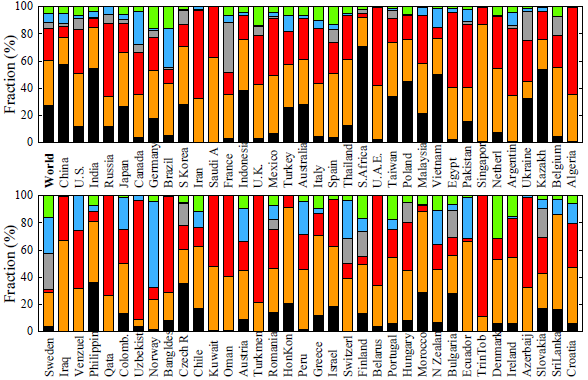
\includegraphics{fig/Energy_Consumption_by_Fuel_2019_World_and_71_Countries_James_Hansen_PlanetCh47.png}

Fig. Energy consumption (percent) in 2019 by fuel in world and 71 nations: BP data
(black = coal, orange = oil; red = gas; gray = nuclear; blue = hydro; green = renewable).
{[}Source:James Hansen: Planet Ch47{]}

\hypertarget{energy-efficiency}{%
\section{Energy Efficiency}\label{energy-efficiency}}

\hypertarget{rebound-effect}{%
\subsection{Rebound effect}\label{rebound-effect}}

Rebound effect = Jevons Paradox

\emph{Lange}

Literature on the rebound phenomenon has grown significantly over the last decade. However, the field is
characterized by diverse and ambiguous definitions and by substantial discrepancies in empirical estimates and
policy proposals. As a result, cumulative knowledge production is difficult. To address these issues, this arti\\
cle
develops a novel typology. Based on a critical review of existing classifications, the typology introduces an
important differentiation between the rebound mechanisms, which generate changes in energy consumption, and
the rebound effects, which describe the size of such changes. Both rebound mechanisms and rebound effects can
be analytically related to four economic levels -- micro, meso, macro and global -- and two time frames -- short r\\
un
and long run. The typology is populated with eighteen rebound mechanisms from the literature. This contribution
is the first that transparently describes its criteria and methodology for developing a rebound typology and th\\
at
gives clear definitions of all terms involved. The resulting rebound typology aims to establish common con-
ceptual ground for future research on the rebound phenomenon and for developing rebound mitigation policies.

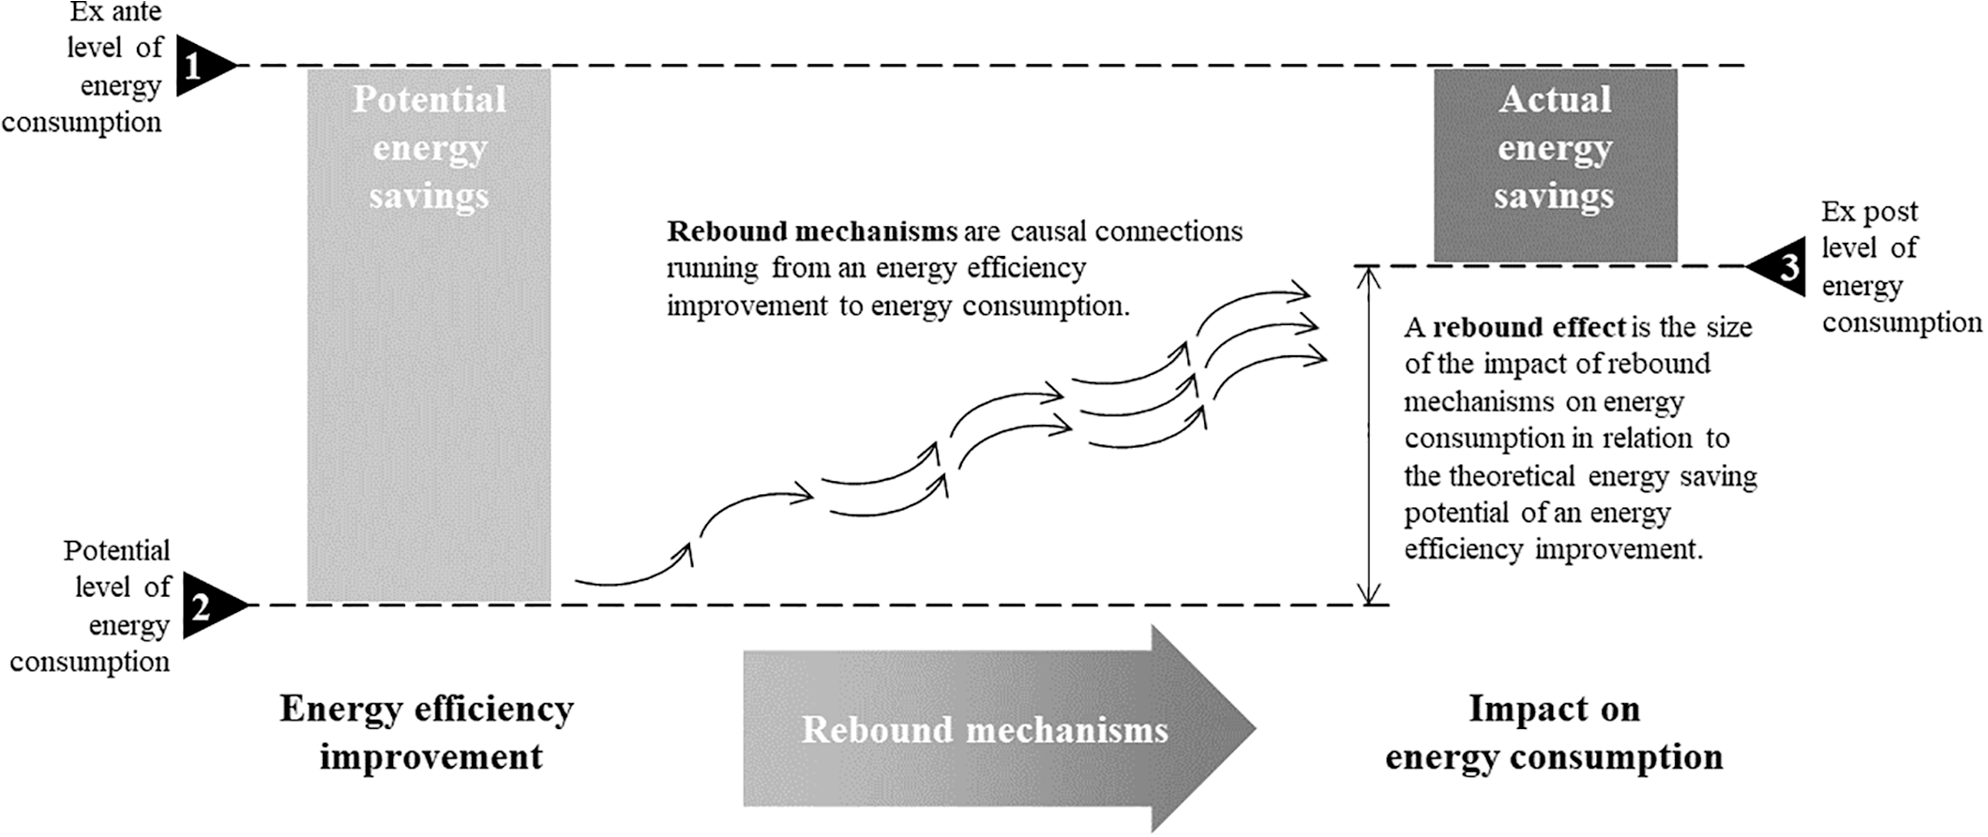
\includegraphics{fig/lange_rebound.png}

Figure: The relationship between energy efficiency improvements, rebound mechanisms and rebound effects. This figure presents the definitions and illustrates the
conceptual distinction between rebound mechanisms and rebound effects. The size of the rebound effect is defined by the relationship between three levels of energy
consumption: 1) ``ex ante'', i.e.~before the efficiency improvement, 2) ``potential'', i.e.~theoretically possible due to the efficiency improvement, and 3) ``ex post'', i.e.
actually realized by the efficiency improvement. Actual savings can be negative in case of backfire. Rebound mechanisms link the energy efficiency improvement to
its actual impact on energy consumption.

While there are a variety of existing classifications of rebounds ef­
fects, few articles have focused on developing coherent and transparent
typologies. This paper aims to advance the foundations of such a ty­
pology by systematically building on existing typologies and being clear
in its definitions and its development. We see our attempt as a step to­
wards developing a shared typology as envisaged by Dunlop {[}3{]}. A
possible next step would be to challenge or advance this typology by
attempting to incorporate non-economic rebound mechanisms and to
see in how far and in what ways it would need to be adjusted. It is our
hope that the transparency of our approach will provoke further critical
debate within the community, at the end of which some form of agreed
typology could emerge.

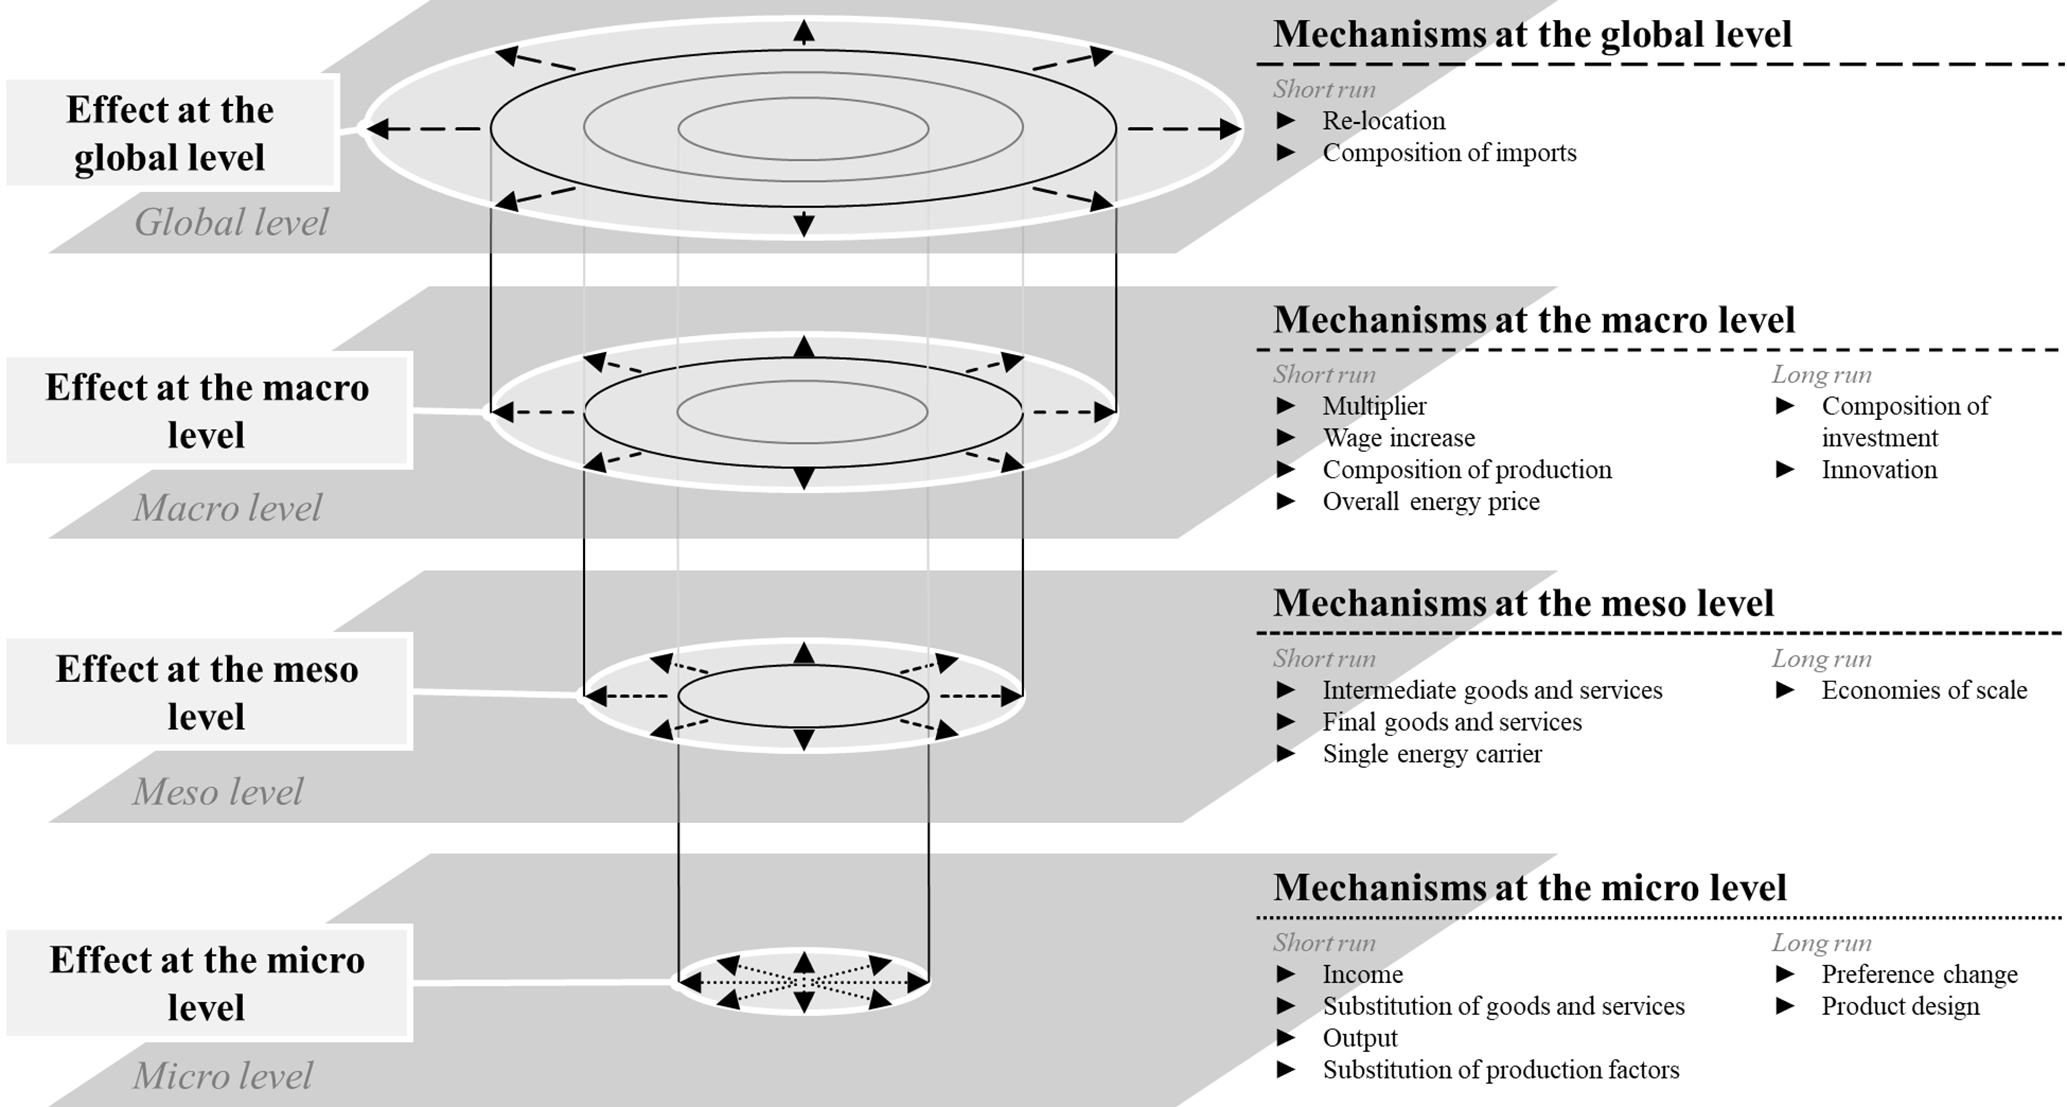
\includegraphics{fig/lange_rebound_levels.png}

Figure: Rebound effects and mechanisms at different economic levels and time frames. This figure provides an overview of the central categories in our typology.
Four stacked analytical levels on which the rebound effect can be measured are distinguished. At each level, several rebound mechanisms, which are represented by
the arrows, cause an increase in energy consumption. The respective types of mechanisms are categorized into short run and long run mechanisms. The connecting
lines between the levels indicate that the rebound effect at a lower level is part of the rebound effect at a higher level.

\href{https://www.sciencedirect.com/science/article/pii/S221462962100075X}{Lange (2021) Jevons Unravelled}
\href{pdf/Lange_2021_Jevons_Unravelled.pdf}{(pdf)}

\hypertarget{urbanization}{%
\section{Urbanization}\label{urbanization}}

\emph{Fix (twitter)}

Are cities sustainable? A loaded question, yes. But one we should think about nonetheless.
Here's an undeniable fact: urbanization correlates strongly with energy use per person.

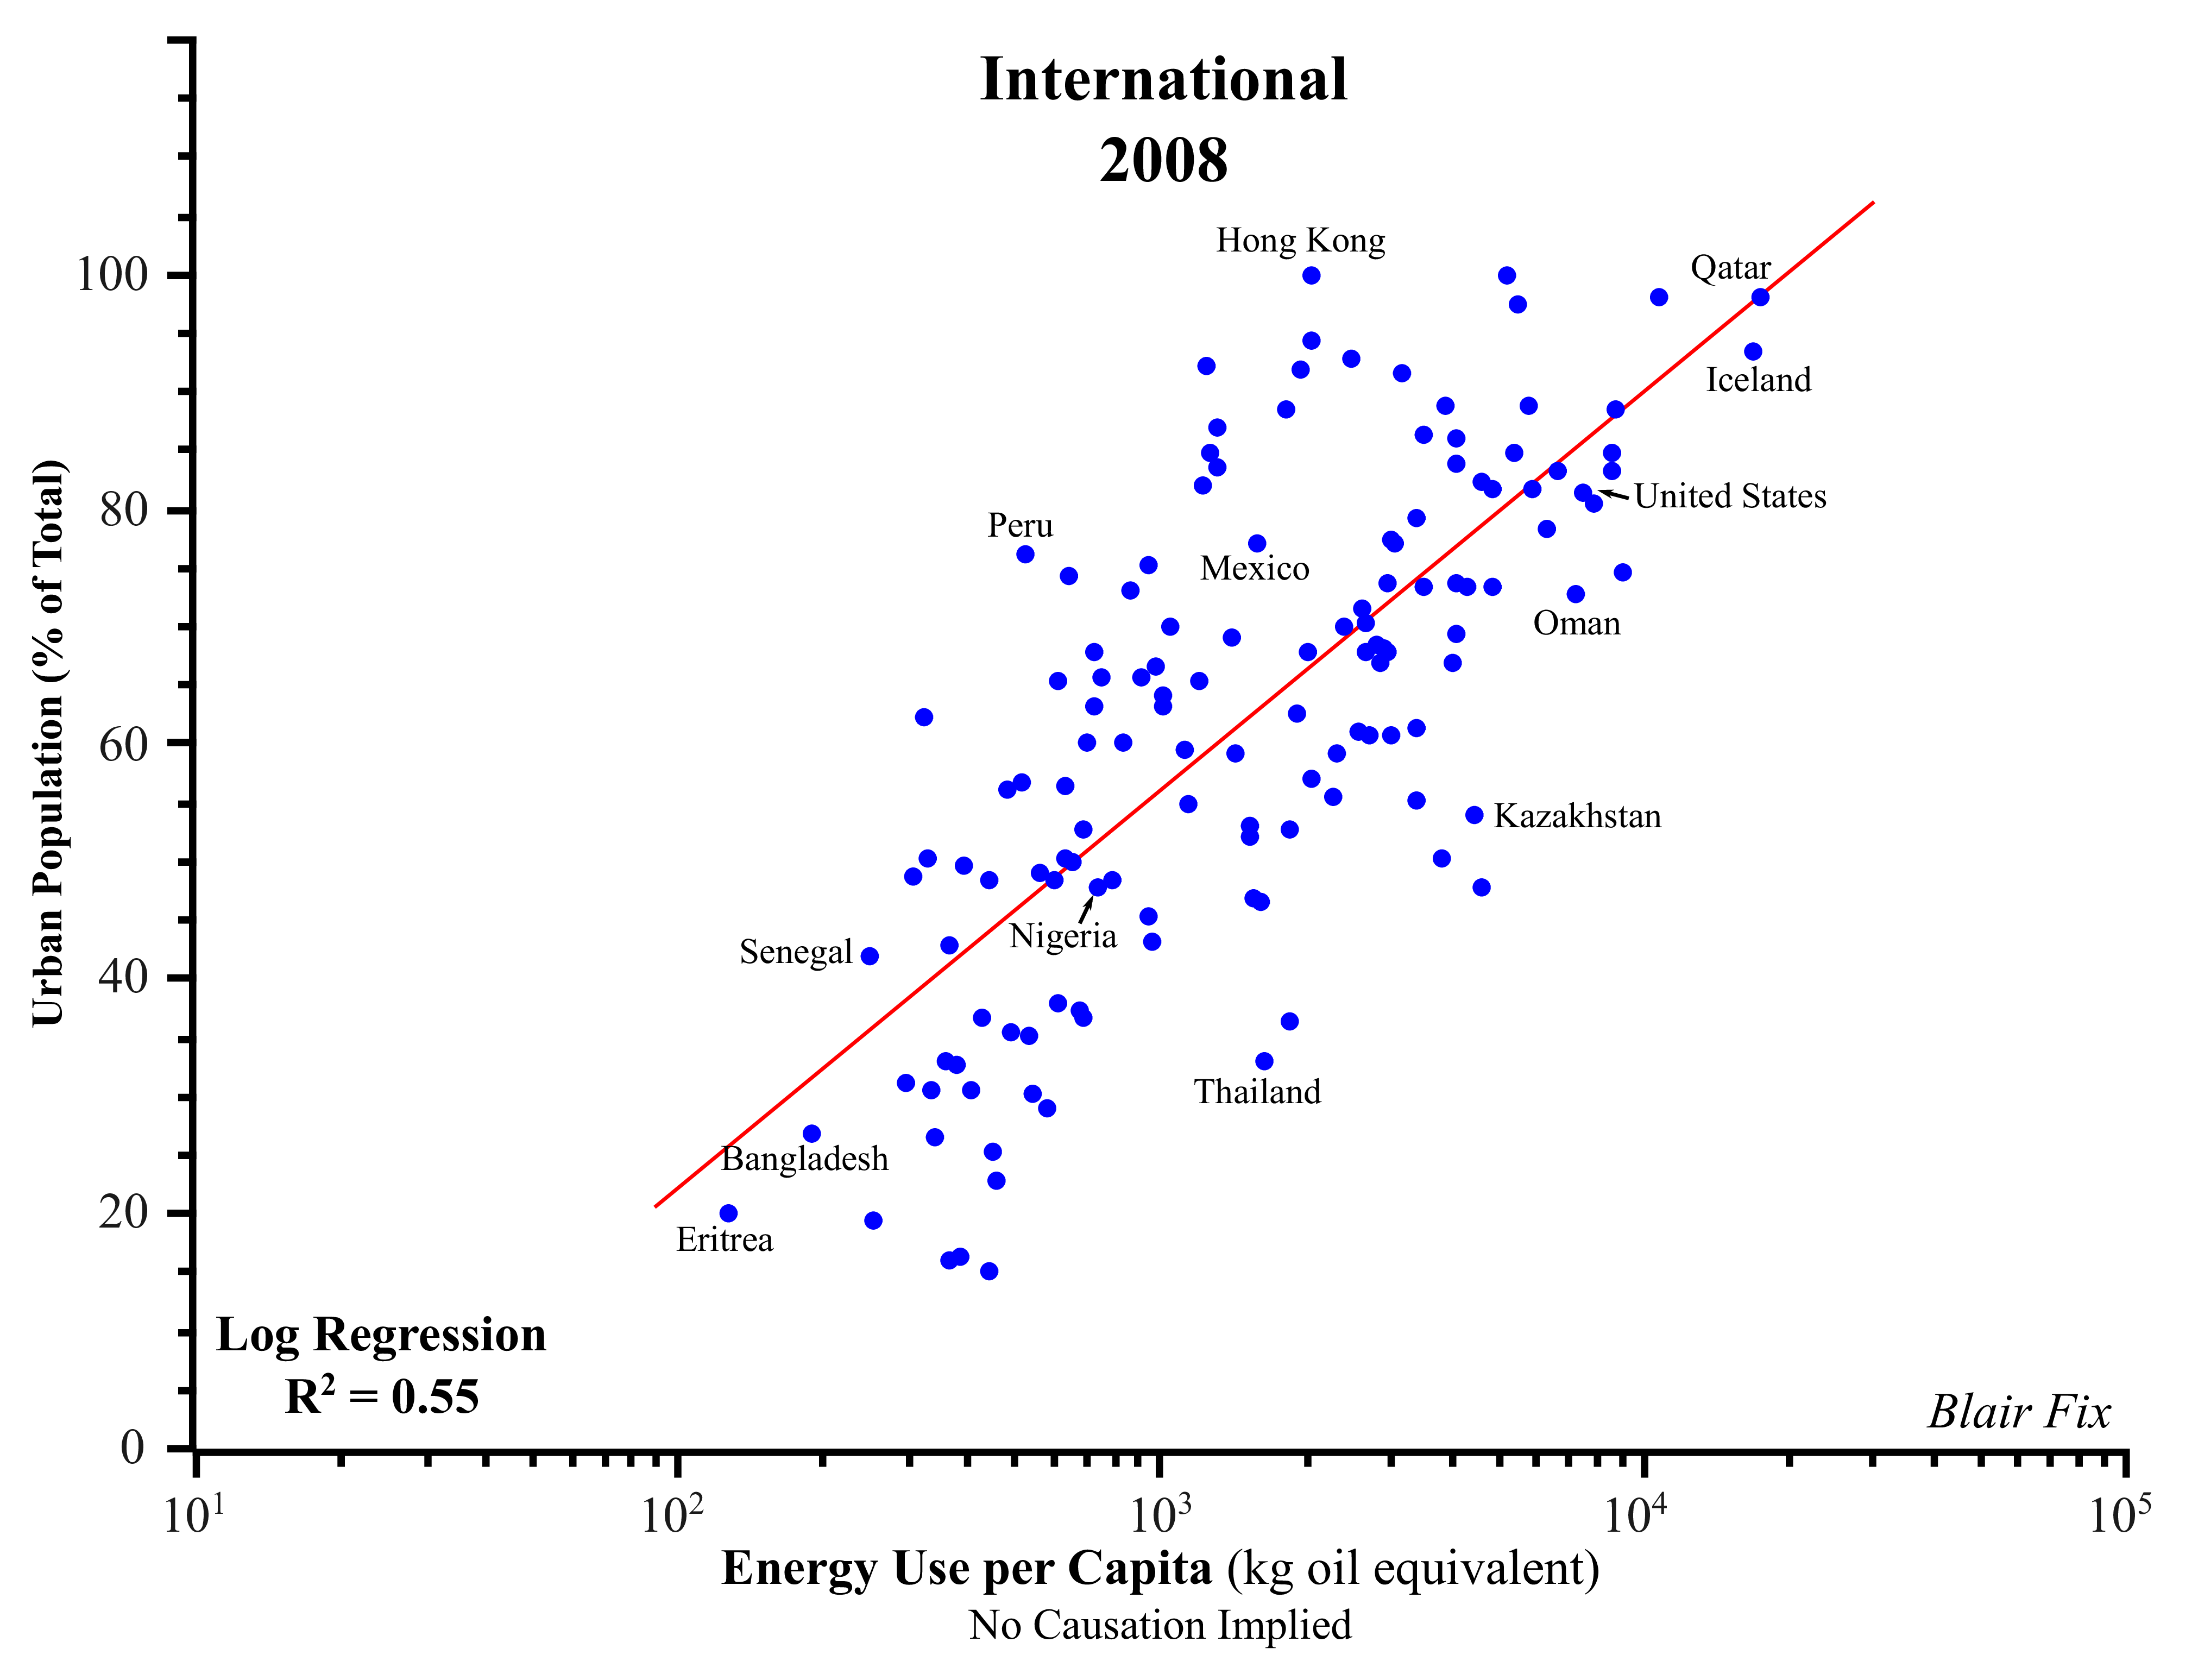
\includegraphics{fig/Fix_2008_Urban_Energy_Use.png}

\hypertarget{green-steel}{%
\section{Green Steel}\label{green-steel}}

\emph{Roselund}

In conventional iron production, blast furnaces use coke --- nearly pure carbon coal --- to heat ore and separate oxygen from the iron in the ore. For this step, Hybrit uses a different, more efficient process called direct reduction. While this can be done with natural gas or even coal as the agent that removes the oxygen, Hybrit's innovation is to use hydrogen made from electrolysis powered by renewable energy. The clean exterior of the facility is a testament to this: Instead of soot from unburned carbon and large amounts of CO2, the Hybrit plant emits clouds of water vapor.

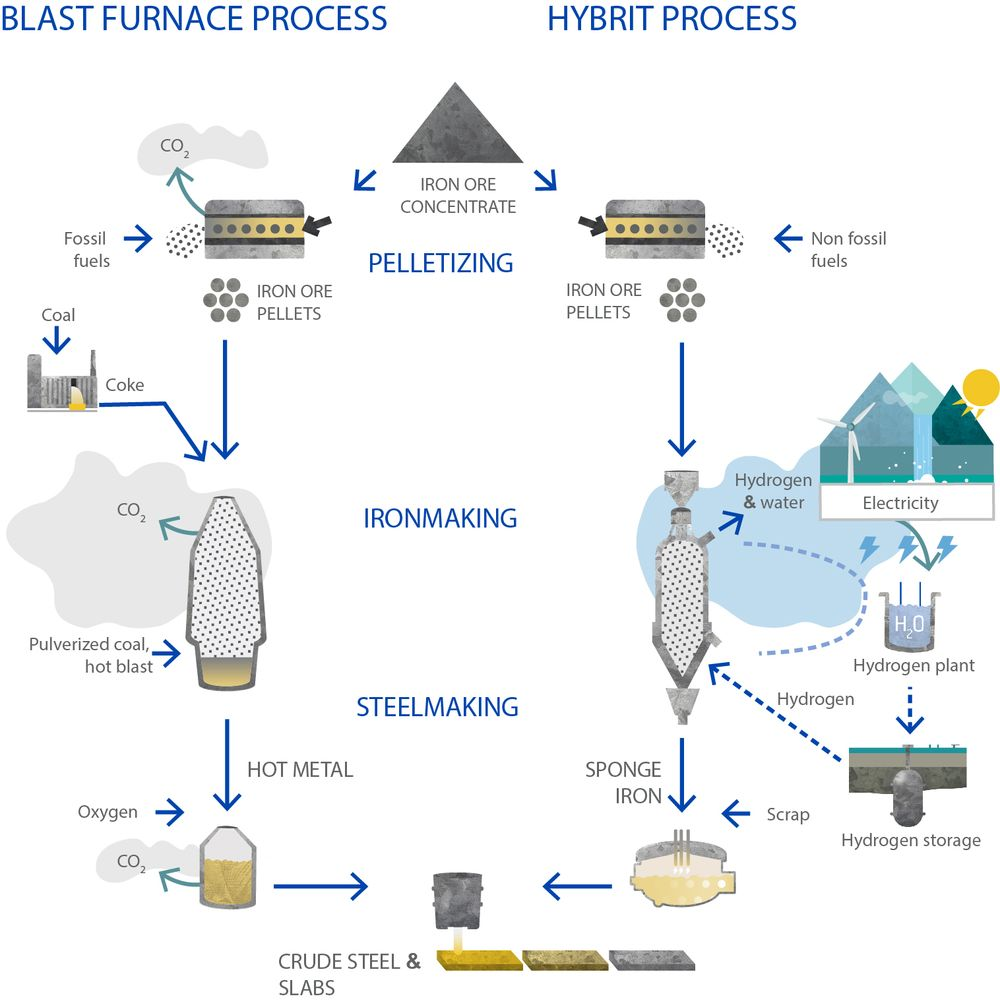
\includegraphics{fig/hybrit-h2-based-ironmaking-en.jpg}

This is groundbreaking. Iron and steel production accounts for 7\% of total global CO2 emissions, and climate and energy experts have long considered it one of the more challenging industries to decarbonize. Recycling of steel can mitigate some of the emissions --- provided furnaces run on electricity from low- or zero-carbon sources --- but will not suffice to meet global demand in the 21st century. Building all of the wind turbines, transmission towers and other infrastructure we need for global decarbonization will require a lot of steel. Additionally, growing economies in China, India and other rapidly developing nations are expected to drive a big increase in steel demand over the next few decades.

\href{https://www.canarymedia.com/articles/green-steel-is-coming-sooner-than-you-think/}{Roselund (2021) Green steel is picking up steam in Europe (CanaryMedia)}

\hypertarget{molten-oxide-electrolysis}{%
\subsection{Molten Oxide Electrolysis}\label{molten-oxide-electrolysis}}

\emph{Soltoff}

Decarbonizing the steel industry is a major hurdle in dealing with climate change. Steel production is responsible for close to 7\% of global greenhouse gas emissions, roughly equivalent to the annual emissions of all the cars on the world's roads. But steel is also used to make cars, so these impacts are overlapping. And that gets to the very heart of why steel is such a big deal when it comes to climate change: It's everywhere.

Decarbonization often comes down to finding creative uses for electricity. The playbook is simple. You take a process that traditionally burns fossil fuels, and then you replace it with an alternative that uses clean electricity instead.

Of course, this is much easier said than done, especially for heavy-duty industrial processes like steel production. In these cases, many solutions rely on green hydrogen as a sort of middleman. You can use clean electricity to produce hydrogen, and then burn hydrogen to make steel, with only water as a byproduct. A joint venture in Sweden is already producing fossil-free steel using this method, though still in relatively small quantities.

One company, MIT spinout Boston Metal, is aiming to streamline the process by eliminating the green-hydrogren step and instead using electricity directly for making steel. Its process is based on technology called molten oxide electrolysis that uses electric current to separate oxygen from iron ore, a critical step in the steel production process.

Boston Metal has already raised \$85 million from climatetech heavyweights like Breakthrough Energy Ventures, The Engine, Prelude Ventures and Energy Impact Partners, along with several industry coalitions and corporate venture groups. It aims to build its first commercial steel plant by 2024 or 2025, and then license its technology to major steel producers.

Producing 1 ton of steel with traditional methods releases almost 2 tons of CO2 into the atmosphere, and the world uses almost 2 billion tons of steel each year.

In the short term, existing steel can be melted down with electricity and reused, which can displace the need for new product --- but only to a point. Most of the world's steel needs can only be met with primary production because recycled steel doesn't work for certain high-grade applications, and more significantly, there's just not enough of it to keep pace with demand.

The traditional way to make steel is to melt iron ore at very high heat (over 1,500 degrees Celsius), then refine it from iron oxide into pure iron and fortify it with small amounts of carbon. It's a complex process that emits carbon at different stages. Some emissions come from the heating process, which usually involves burning a heat-refined form of coal called coke. A bit of the carbon from the coke gets dissolved into the iron, turning it into steel. Another chunk of emissions comes from chemical reactions that occur as the iron oxide is purified of its chemically bonded oxygen. That oxygen reacts with dissolved carbon and breaks off as carbon dioxide gas.

Over half of the emissions come from a single piece of equipment used in the process: the blast furnace, where the iron ore is converted into a form called pig iron.
Decarbonization of the iron and steel industry basically means decarbonization of the blast furnace.

Green hydrogen appears to be the most promising route to decarbonizing steel, with hydrogen-powered direct reduction of iron as a key step in cutting the emissions from blast furnaces. This process is now being used in green steel projects in Europe, and some of China's biggest steelmakers are exploring it as well.
Molten oxide electrolysis is too nascent.

The core principle of using electricity to refine metal has been around for a while. In fact, electrolysis has been a key part of making aluminum for over 100 years. Boston Metal's molten oxide electrolysis process applies this technique to iron, which requires hotter temperatures. Aluminum electrolysis happens at temperatures just under 1,000 degrees Celsius, while iron electrolysis requires about 1,600°C, a temperature far hotter than molten lava.

To start, the iron ore is melted with heat produced from electricity. Then it's placed in a cell structured almost like a giant battery. At the top, an anode provides electric charge. At the bottom, a cathode receives the electric charge. In between, the charge flows through an electrolyte, which in this case is a scalding bath of molten materials. The electrolyte contains a variety of elements bound to oxygen, including aluminum, silicon and calcium.

All of these oxides are more stable than iron oxide, so the iron oxide is the first to separate when exposed to electric charge, breaking down into pure oxygen and iron. The iron, still liquified, sinks to the bottom where it can be tapped out and turned to steel.

The composition of the electrolyte is a critical advantage of its technology. All of those other elements in the electrolyte are also present in iron ore as impurities, but the impurities stay behind in the electrolyte after the pure iron is removed. That means the process works even with low-grade iron ore, which is cheaper and more plentiful than higher-grade ore that has fewer impurities.

Another of molten oxide electrolysis's advantages compared to direct reduction of iron is its efficiency. The reason is fairly intuitive. By cutting out the hydrogen step, MOE puts energy directly into steel production, removing interim stages where energy can be lost. MOE requires higher temperatures than hydrogen-based production, which eats into the benefits, but even taking that into account, MOE still winds up being more efficient. Making green steel using green hydrogen requires at least 30\% more energy than MOE --- and possibly as much as 50\% to 60\% more.

Boston Metal says that its technology uses 4 megawatt-hours of electricity to produce 1 ton of steel.
According to Columbia's research on decarbonizing steel, replacing all the world's blast furnaces with MOE manufacturing processes would require an amount of power equivalent to almost 20 percent of global electricity consumption in 2018. That means the steel industry would become one of the biggest users of electricity on the planet.

But replacing all steel production with hydrogen-powered direct reduction of iron could require even more electricity. That means there's no way to address steel's climate impacts without installing a whopping amount of clean power generation, in addition to making sure that the grid is ready to reliably move around all that extra electricity.

\href{https://www.canarymedia.com/articles/clean-industry/green-steel-without-green-hydrogen-can-it-work}{Soltoff (2022) Green steel without green hydrogen --- can it work?}

\hypertarget{energy-poverty}{%
\chapter{Energy Poverty}\label{energy-poverty}}

Without cheap, safe, low-carbon energy sources at scale
we are stuck between the alternatives of high greenhouse gas emissions
and energy poverty.

The world lacks safe, low-carbon, and cheap large-scale energy alternatives to fossil fuels. Until we scale up those alternatives the world will continue to face the two energy problems of today. The energy problem that receives most attention is the link between energy access and greenhouse gas emissions. But the world has another global energy problem that is just as big: hundreds of millions of people lack access to sufficient energy entirely, with terrible consequences to themselves and the environment.

The richest 1\% in the EU emit on average 43 tonnes of CO2 annually -- 9-times as much as the global average of 4.8 tonnes.
The problem is larger for the extremely rich.

The only countries that have emissions that are close to zero are those where the majority suffers from energy poverty.

\href{https://ourworldindata.org/worlds-energy-problem}{Roser (2021) The World's Energy Problem}

\hypertarget{carbon-intensity-of-energy}{%
\chapter{Carbon intensity of Energy}\label{carbon-intensity-of-energy}}

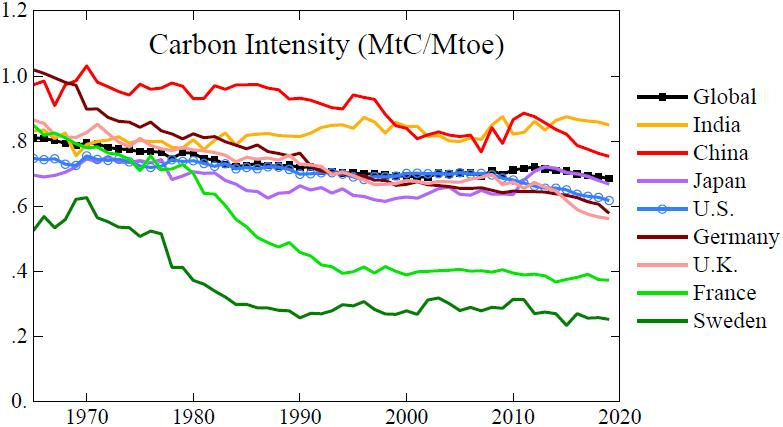
\includegraphics{fig/carbon_intensity_James_Hansen_planetCh47.jpg}

That chart -- fossil fuel carbon (GtC) emitted per
unit energy (Gt of oil equivalent) -- is arguably the best summary of how well the world is doing
in moving to carbon-free energy. Atmospheric CO 2 may approximately stabilize when we reach
a carbon intensity near 0.25, but carbon intensity must be closer to zero to draw down
atmospheric CO 2 and cool Earth to a level that stabilizes ice sheets and terminates tundra melt.
Unfortunately, global carbon intensity remains stubbornly high -- almost 0.7 -- in part because
emerging economies, such as China and India, get much of their energy from coal. Moreover,
progress in reducing carbon intensity is inadequate in most nations worldwide.
Sweden is a notable exception. How did Sweden do it? Once, when a Swedish minister showed
a graph similar to Fig. 47.5, I asked how they achieved the rapid drop of carbon emissions
between the mid-1970s and mid-1980s? The answer: ``we introduced combined heat and
power.'' Wonderful! This suggests that if we get the rest of the world to adopt combined heat
and power, the global warming problem will be almost solved.
Eh, not so much. A Swedish engineer told me that the main reason was that Sweden completed
10 nuclear power plants in that decade. I interpreted the conflicting answers as a difference
between scientists and ministers. The scientist looks at numbers and facts objectively, while the
minister bears politics in mind, and the Swedish government had become quite anti-nuclear.
Both answers were true, but the minister was misleading -- hiding the crucial information.

{[}James Hansen: Sophies Planet Ch.47{]}

\hypertarget{rebound-effect-1}{%
\chapter{Rebound Effect}\label{rebound-effect-1}}

First, note that when an energy service becomes more efficient, it also becomes less expensive. Say I trade in my old car in for a Prius, which is 20 percent more fuel efficient. Among other things, that means I spend (roughly) 80 percent what I used to spend to drive how much I used to drive.

That's money in my pocket I didn't have before. What do I do with it?

One thing I might do with it is buy more gas, i.e., drive more. In other words, I might respond to the lower cost of an energy service by increasing my demand for the service. The amount of primary energy I use for driving, which fell when I bought my Prius, would rebound back upward. That is the direct rebound effect.

Or, I might use the extra money to, say, buy an iPad. Thing is, manufacturing and operating an iPad requires energy. So even if the energy I devote to driving drops, my total energy use could rebound back upward. That is the indirect rebound effect.

(The same basic story applies to businesses. If their energy costs go down through energy efficiency, they invest some of the savings in more production, thus bumping their energy use back up.)

Stepping back, there's the question of economy-wide rebound effects. If we drive energy efficiency across the entire economy, then we lower what's called the energy intensity of the economy, that is, how much primary energy it takes to get a unit of GDP. When the economy as a whole is more energy efficient, it takes less energy to create wealth.

What is the macroeconomic effect of a drop in energy costs? The same effect we'd expect from a drop in labor costs or capital costs: faster growth. And insofar as stimulating growth means increasing energy use, that will wipe out some of the energy-saving gains of the efficiency.

\href{https://grist.org/energy-efficiency/whats-the-deal-with-the-rebound-effect/}{David Roberts}

\hypertarget{fossil-subsidies}{%
\chapter{Fossil Subsidies}\label{fossil-subsidies}}

This paper estimates the financial benefits accruing to fossil fuel producers (i.e., the producer incidence) that arise because of implicit fossil fuel subsidies in the United States. The analysis takes account of coal, natural gas, gasoline, and diesel, along with the implicit subsidies due to externalized environmental damages, public health effects, and transportation-related costs. The direct benefit to fossil fuel producers across all four fuels is estimated at \$62 billion per year, a sum calculated due to the higher price that suppliers receive because of inefficient pricing compared to the counterfactual scenario where environmental and public health externalities are internalized. A significant portion of these benefits accrue to relatively few companies, and specific estimates are provided for companies with the largest production. The financial benefit because of unpriced costs borne by society is comparable to 18\% of net income from continuing domestic operations for the median natural gas and oil producer in 2017--2018, and it exceeds net income for the majority of coal producers. The results clarify what the domestic fossil fuel industry has at stake financially when it comes to policies that seek to address climate change, adverse health effects from local pollution, and inefficient transportation.

\textbf{Producer Incidence}

The producer benefits of interest---i.e., the producer incidence (PI)---are based on the higher price that suppliers receive because of inefficient pricing compared to the counterfactual scenario where environmental and public health externalities are internalized. The direct financial benefit to fossil fuel producers of inefficient pricing across all four fuels is estimated at \$62 billion per year on average,
representing 11\% of the total annual subsidy of \$568 billion. The total subsidy is equivalent to an average of 3\% of US Gross Domestic Product and equals the estimated value of the environmental, public health, and transportation-related externalities on an annual basis. To be clear, the focus here is not on direct subsidy payments that reduce the costs of fossil fuels, but rather on the implicit subsides that arise because of inefficient pricing that gives rise to social costs (1, 2, 6). While direct subsidy payments are common in many countries (7⇓--9), they are not in the United States.

This paper also makes two methodological contributions to the literature on fossil fuel subsidies. First is a generalization and implementation of the standard International Monetary Fund (IMF) framework to separately estimate the PI and consumer incidence (CI). A key feature of existing studies---which focus on economic efficiency, environmental and health impacts, and government revenues---is the simplifying assumption of perfectly elastic supply. This implicitly assumes away fundamental concerns about the extent to which the fossil fuel industry benefits from subsidies and may therefore seek to prevent reform. The approach taken here uses empirically based estimates of supply elasticities to examine distributional implications, with a focus on PI.

\textbf{Conceptual Framework}

Implicit fossil fuel subsidies represent a hybrid of the standard tax and subsidy scenarios. This follows because externality-based, fossil fuel subsidies arise because of failure to implement efficient pricing, which confers an implicit subsidy. While different mechanisms are possible to establish efficient pricing, the most straightforward to illustrate the key points is Pigouvian taxation. Consider the market for a particular fossil fuel, characterized by the supply and demand curves in Fig. 1A. The initial equilibrium occurs at price p' and quantity Q', which is not efficient because of external costs in the form of environmental damages and adverse health effects. Assume for simplicity that the marginal external costs, denoted MEC, are constant. A Pigouvian tax equals the MEC and places a wedge between the supply and demand curves. If implemented, the Pigouvian tax would establish the efficient quantity Q∗ as the equilibrium and the prices buyers pay and sellers receive as pb∗ and ps∗, respectively.

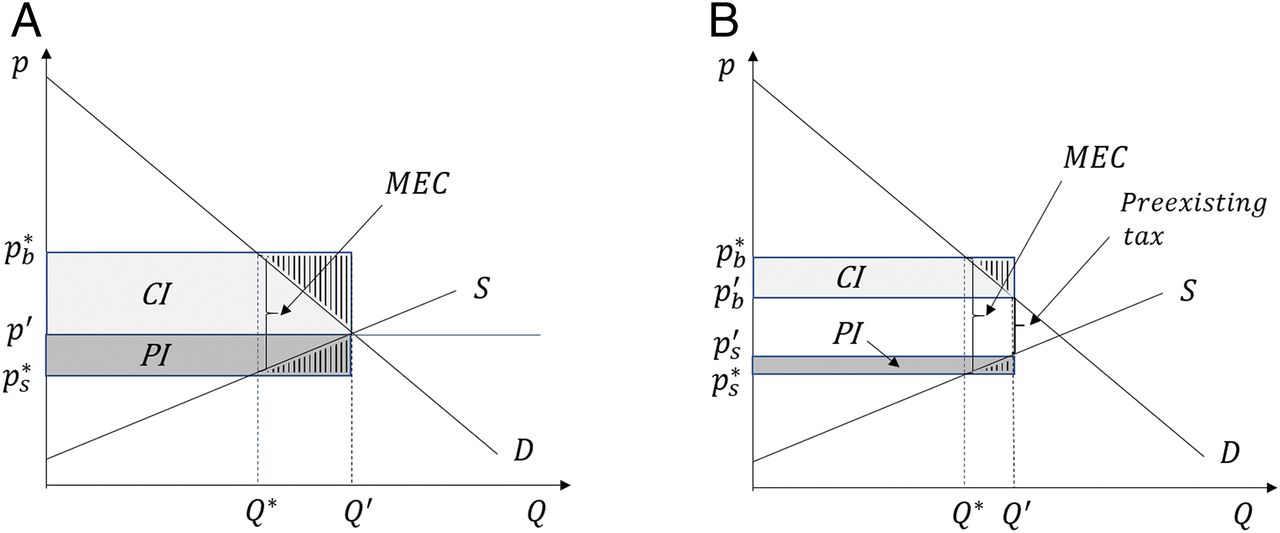
\includegraphics{fig/fossil_subsidy.jpg}

\emph{Figure: The PI and CI of an implicit fossil fuel subsidy. MEC represents the marginal external cost associated with each unit of Q. (A) The presence of no preexisting tax is assumed. The total implicit subsidy is the area MEC×Q'. The incidence measures capture the gain in producer and consumer surplus from inefficient pricing, i.e., the respective shaded areas excluding the vertically hashed triangles. (B) A case with a preexisting tax; the net corrective tax is the difference between the MEC and the preexisting tax.}

The implicit fossil fuel subsidy is defined as the sum of all shaded areas in Fig. 1A; i.e., the rectangle equal to MEC×Q'. This is an effective subsidy because it represents real costs borne by society---through environmental damages and adverse public health effects or foregone tax revenue---but not reflected in the market (1, 10). Of central interest here is the way that the total subsidy differentially benefits consumers and producers (i.e., the measures of incidence). The CI captures the change in net benefits to consumers (i.e., consumer surplus) because of the lower price they pay, and the PI captures the change in net benefits to producers (i.e., producer surplus) because of the higher price they receive. These measures are illustrated in Fig. 1A as the shaded areas labeled CI and PI, respectively, which do not include the vertically hashed triangles. The two regions represent the net gain to consumers and producers of maintaining inefficient pricing.

Previous research nevertheless implicitly assumes the PI is zero, which follows because of the simplifying assumption of perfectly elastic supply (1, 2, 6, 8⇓--10). The assumption is reasonably motivated in previous analyses because of the focus on efficiency rather than distributional concerns between producers and consumers. The assumption is also reasonable in cases where the focus is on relatively small countries subject to the global supply of fossil fuels. The assumption does not, however, fully characterize markets in the United States, especially when it comes to coal and natural gas, which are less interconnected in a global market compared to oil. While less is known about supply elasticities compared to those for demand, existing research does provide a basis for informed assumptions that push away from the limiting case of perfect elasticity, especially for the United States.

A final piece of the model to consider is the possibility for preexisting subsidies or taxes. An explicit, preexisting subsidy would be a direct government payment to reduce the producer or consumer costs of fossil fuels, but as mentioned previously, these are not common in the United States. Instead, implicit market subsidies do arise because of existing tax preferences for oil and gas firms, which have been estimated to cost the US government roughly \$4 billion annually in foregone revenue (11). These subsidies are not accounted for in the present analysis because of the focus on nonmarket implicit subsidies. There are, however, preexisting taxes that affect the immediate applicability of Fig. 1A, and these must be taken into account to get an accurate measure of the fossil fuel subsidy in each case. Fig. 1B generalizes the framework to show how existing tax revenue associated with the initial equilibrium at Q' is not included in the overall subsidy. In this case, the implicit subsidy is based on the net corrective tax (i.e., MEC minus the preexisting tax). The measures of incidence differ as shown but still represent the difference in the respective surplus measures.

\textbf{Overall Producer Incidence}

The methodological approach for estimating the incidence of fossil fuel subsidies requires several steps, all of which are described in detail in SI Appendix. First is obtaining price and quantity data for the different fuels. Second is estimating the MEC associated with each fuel. Third is obtaining information on preexisting taxes in order to calculate the net corrective taxes. Fourth is an approach for generating counterfactual prices that would emerge with efficient pricing. Last is obtaining estimates of supply and demand elasticities.

\textbf{Total Subsidy}

The results indicate a total subsidy across all four fuels of \$592 billion in the most recent year, 2018. This number represents the external costs borne by society or foregone government revenue from inefficient pricing. Included in the external costs is the value of climate damages reflected in the social cost of carbon and adverse health effects from local pollution (SI Appendix, Fig. S1). The external costs for gasoline and diesel also include the value of congestion-based travel delays and accident fatalities, along with wear and tear on the roadways from heavy-duty, diesel fuel vehicles (SI Appendix, Fig. S1).

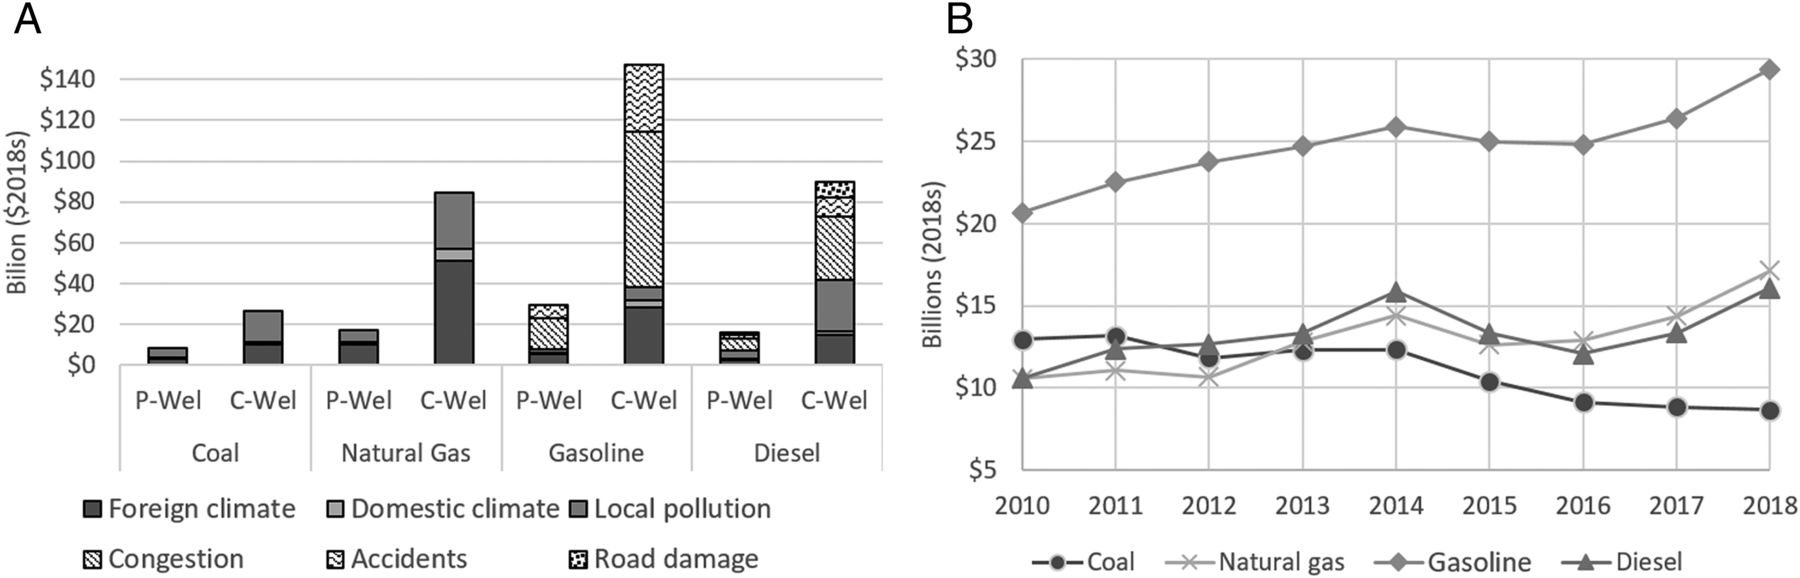
\includegraphics{fig/fossil_subsidy_2.jpg}

\emph{Figure: The PI and CI of the subsidy for all fuels. (A) The measures of PI and CI for all four fuels (coal, natural gas, gasoline, and diesel) for the most recent year, 2018. Data for all other years are available in SI Appendix. Each measure is further partitioned into the underlying externalities, which are proportionally the same between both measures of incidence for each fuel (SI Appendix, Fig. S1). (B) The trend in PI over time for each fuel. While the producer benefits to coal have decreased 33\%, those for all other fuels have increased substantially: 42\% for gasoline, 52\% for diesel, and 63\% for natural gas.}

\href{https://www.pnas.org/content/118/14/e2011969118}{Kotchen (2021) Producer Benefits}
\href{pdf/Kotchen_2021_Fossil_Subsidies.pdf}{(pdf)}
\href{pdf/Kotchen_2021_Fossil_Subsidies_SI.pdf}{SI (pdf)}

\hypertarget{germany}{%
\chapter{Germany}\label{germany}}

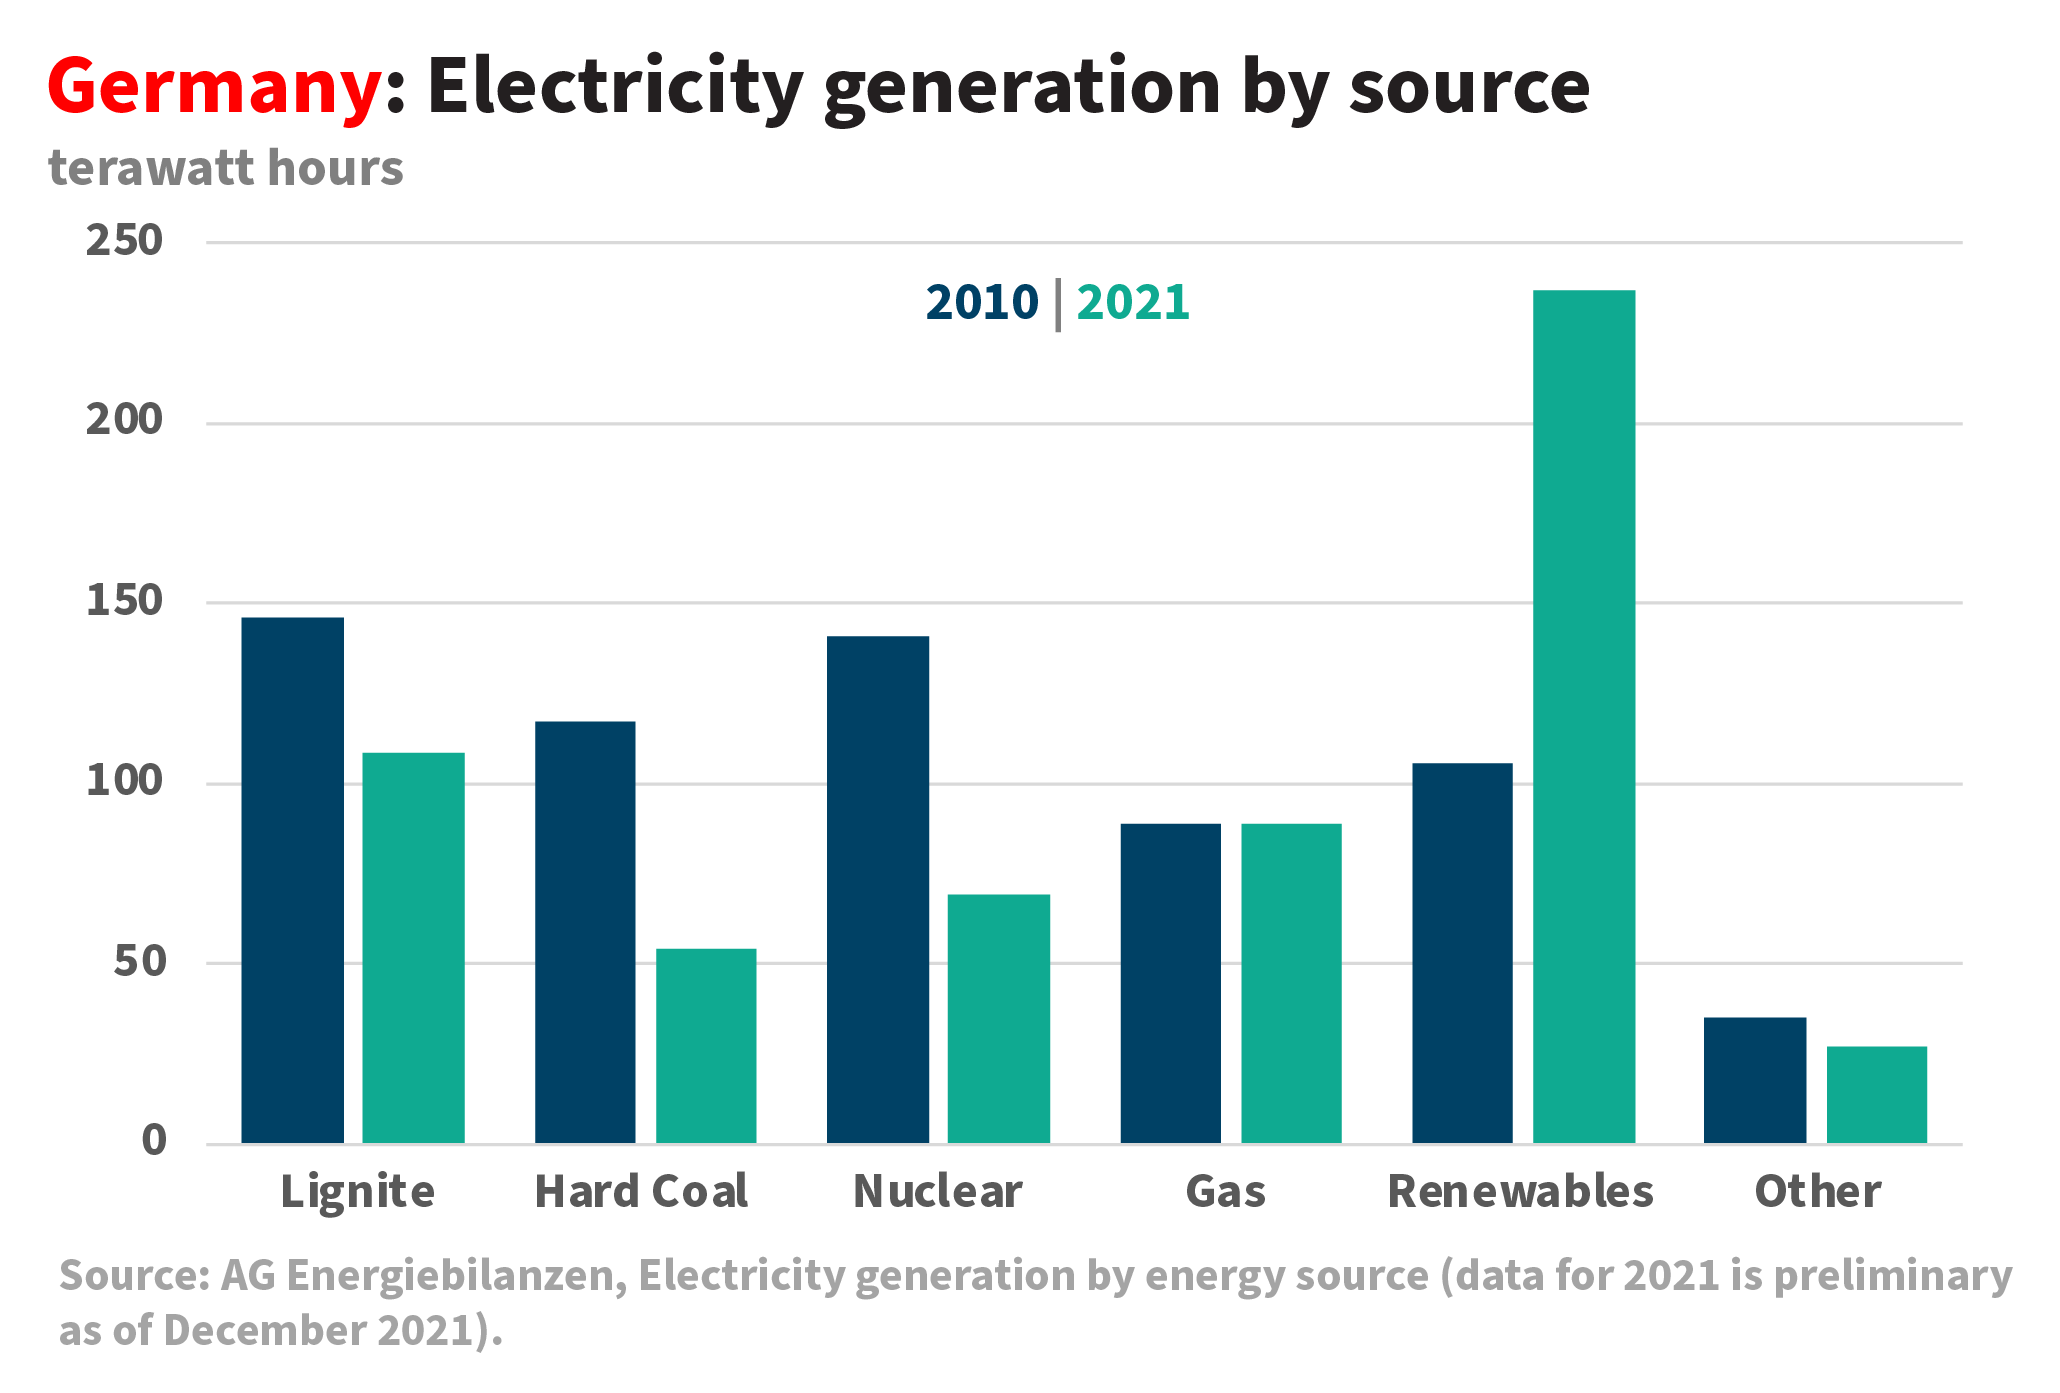
\includegraphics{fig/Germany_2010_2021_Electricty_by_Source.png}

\hypertarget{norway}{%
\chapter{Norway}\label{norway}}

\hypertarget{energy-statistics-1}{%
\section{Energy Statistics}\label{energy-statistics-1}}

\emph{Energifakta.no}

Access to reasonably priced hydropower has shaped energy use in Norway. Everyone has access to electricity, which is used for more purposes than in most other countries. Norway has a large energy-intensive manufacturing sector, and electricity is much more widely used to heat buildings and water than in other parts of the world. Because such a large proportion of electricity is produced from renewable sources, greenhouse gas emissions associated with stationary energy use are low in Norway.

Norway's population has risen by nearly 1 million since 1990 - 22.3\%.

\begin{verbatim}
1990: 4.241.473
2015: 5.188.607 
\end{verbatim}

Strong economic growth has resulted in a doubling of GDP since 1990. Both production of and demand for goods and services that use energy are growing steadily.
However, final energy consumption has risen by only 16 \%, so that the Norwegian economy has become gradually less energy-intensive.

\href{https://energifaktanorge.no/en/norsk-energibruk/}{Energifakta.no}

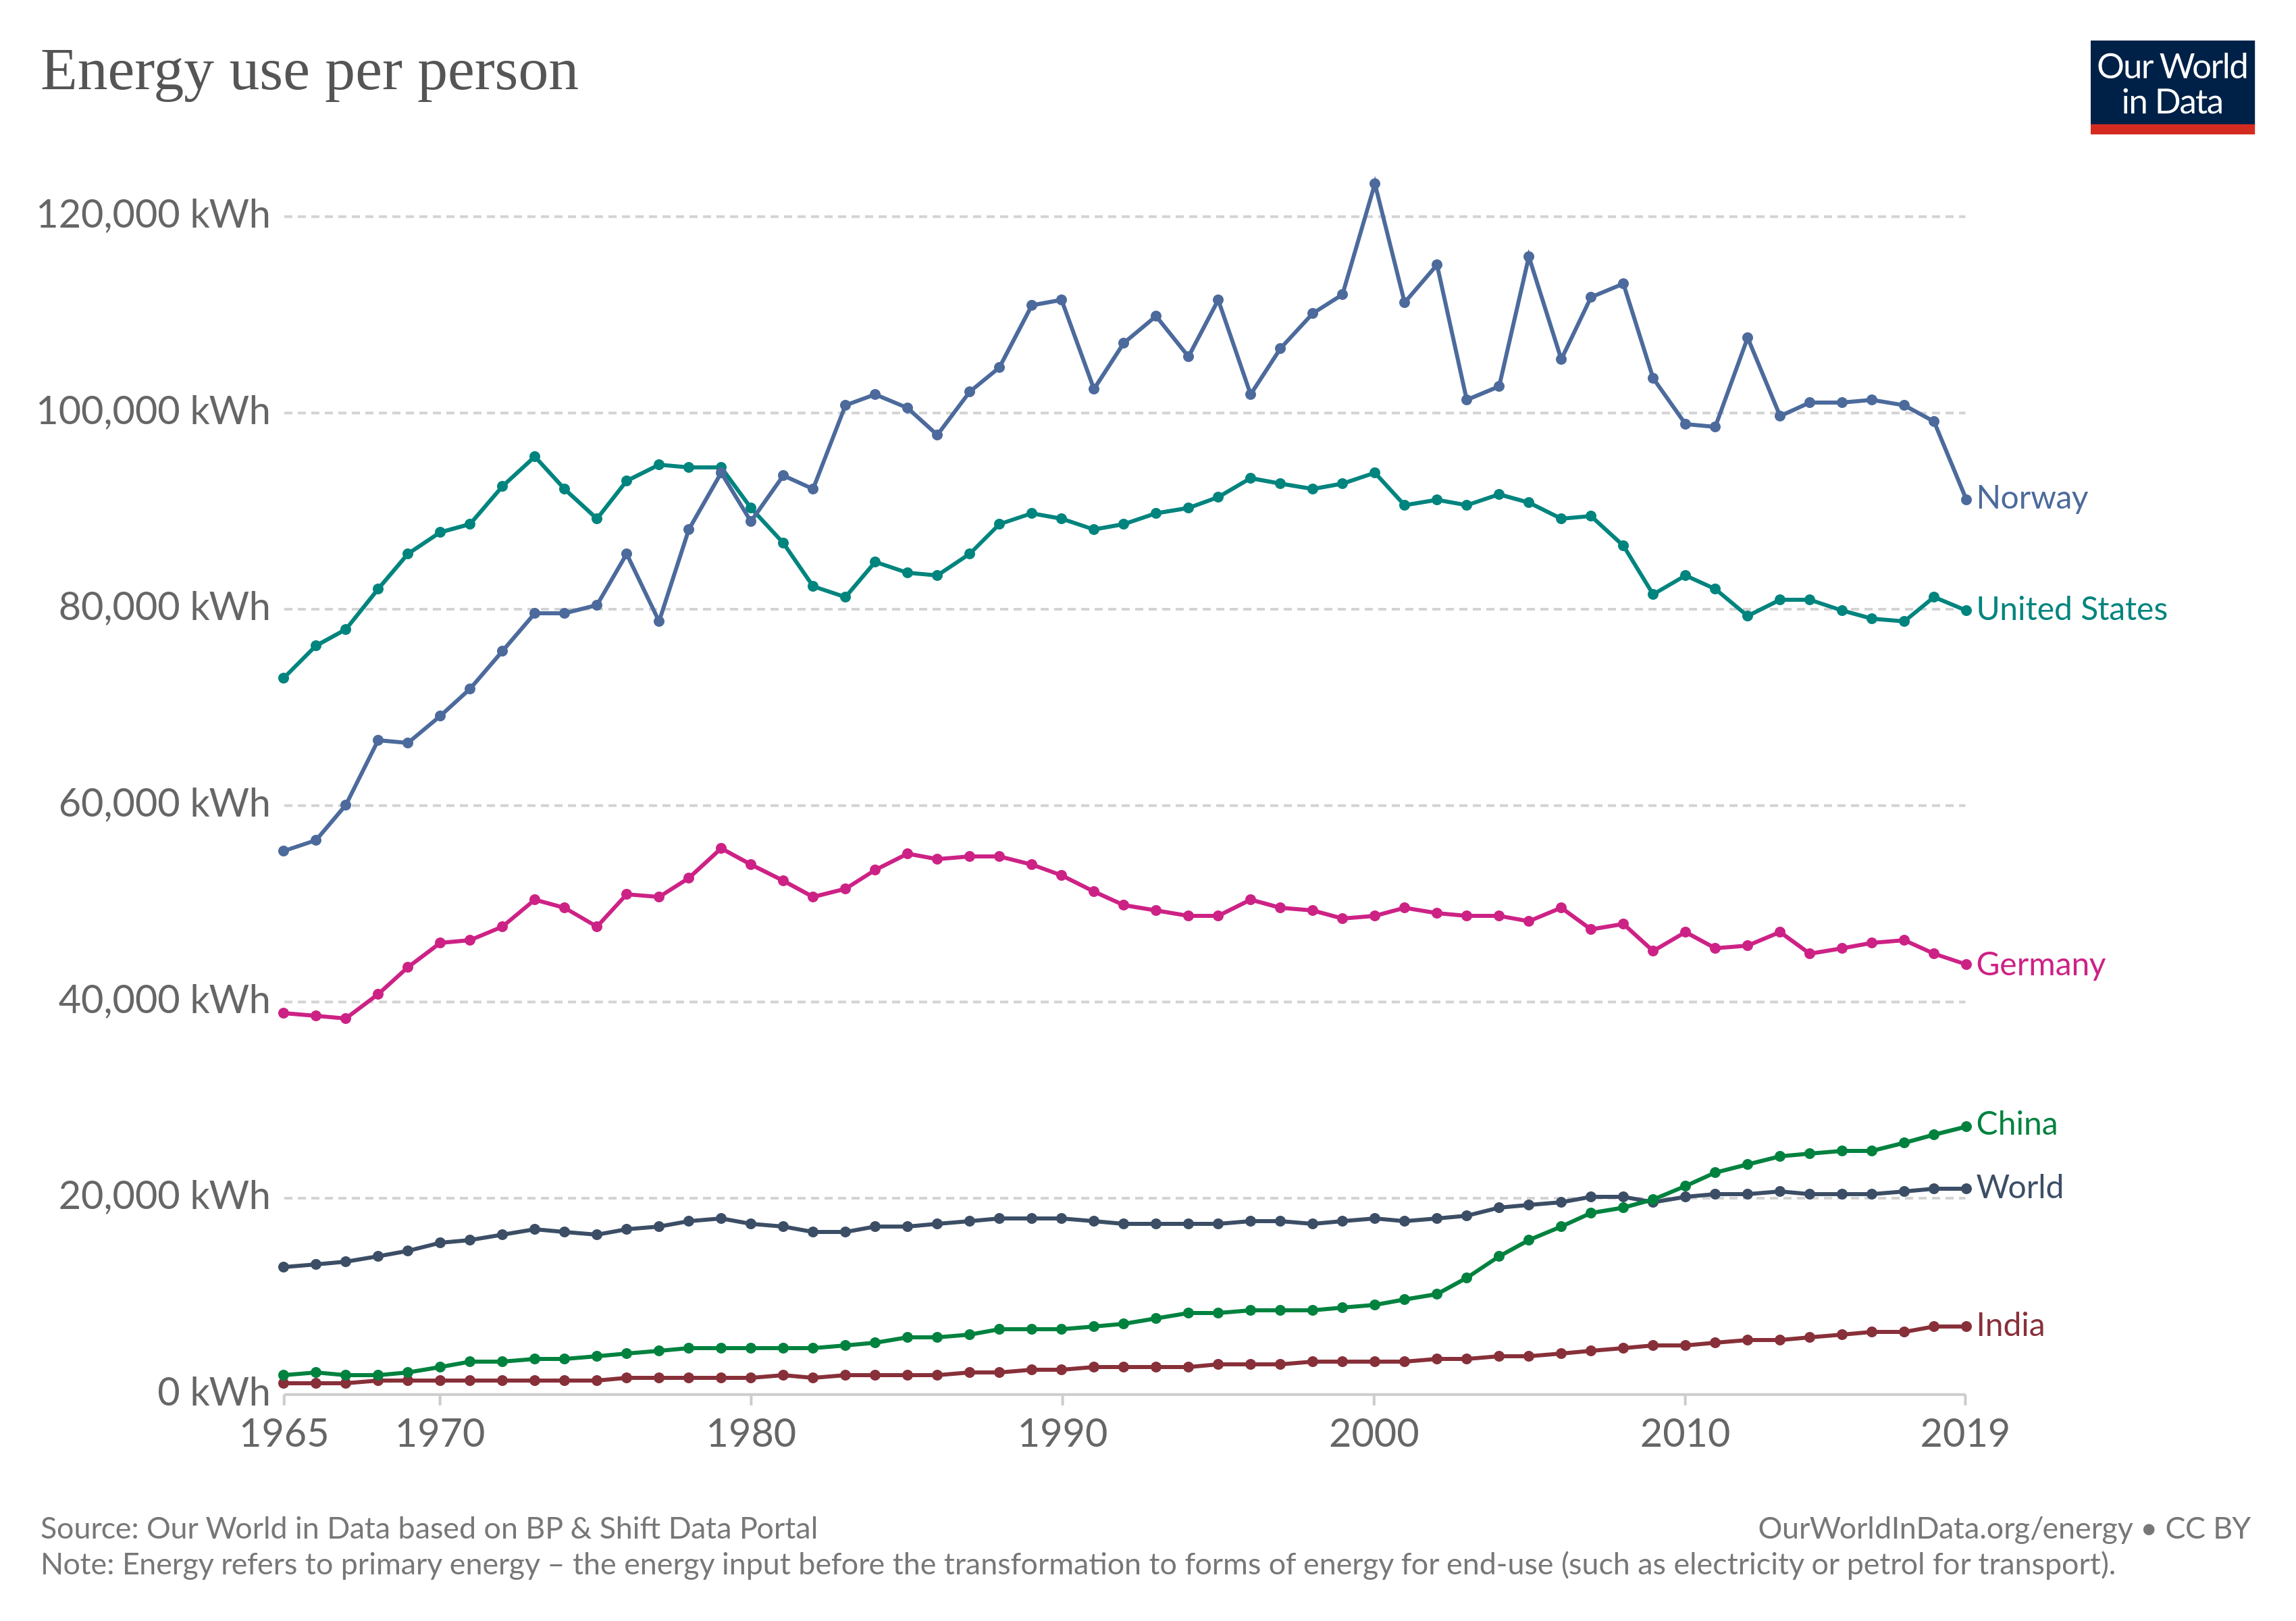
\includegraphics{fig/owid_energy_use_pc_no_us_de_ch_in-wd.png}

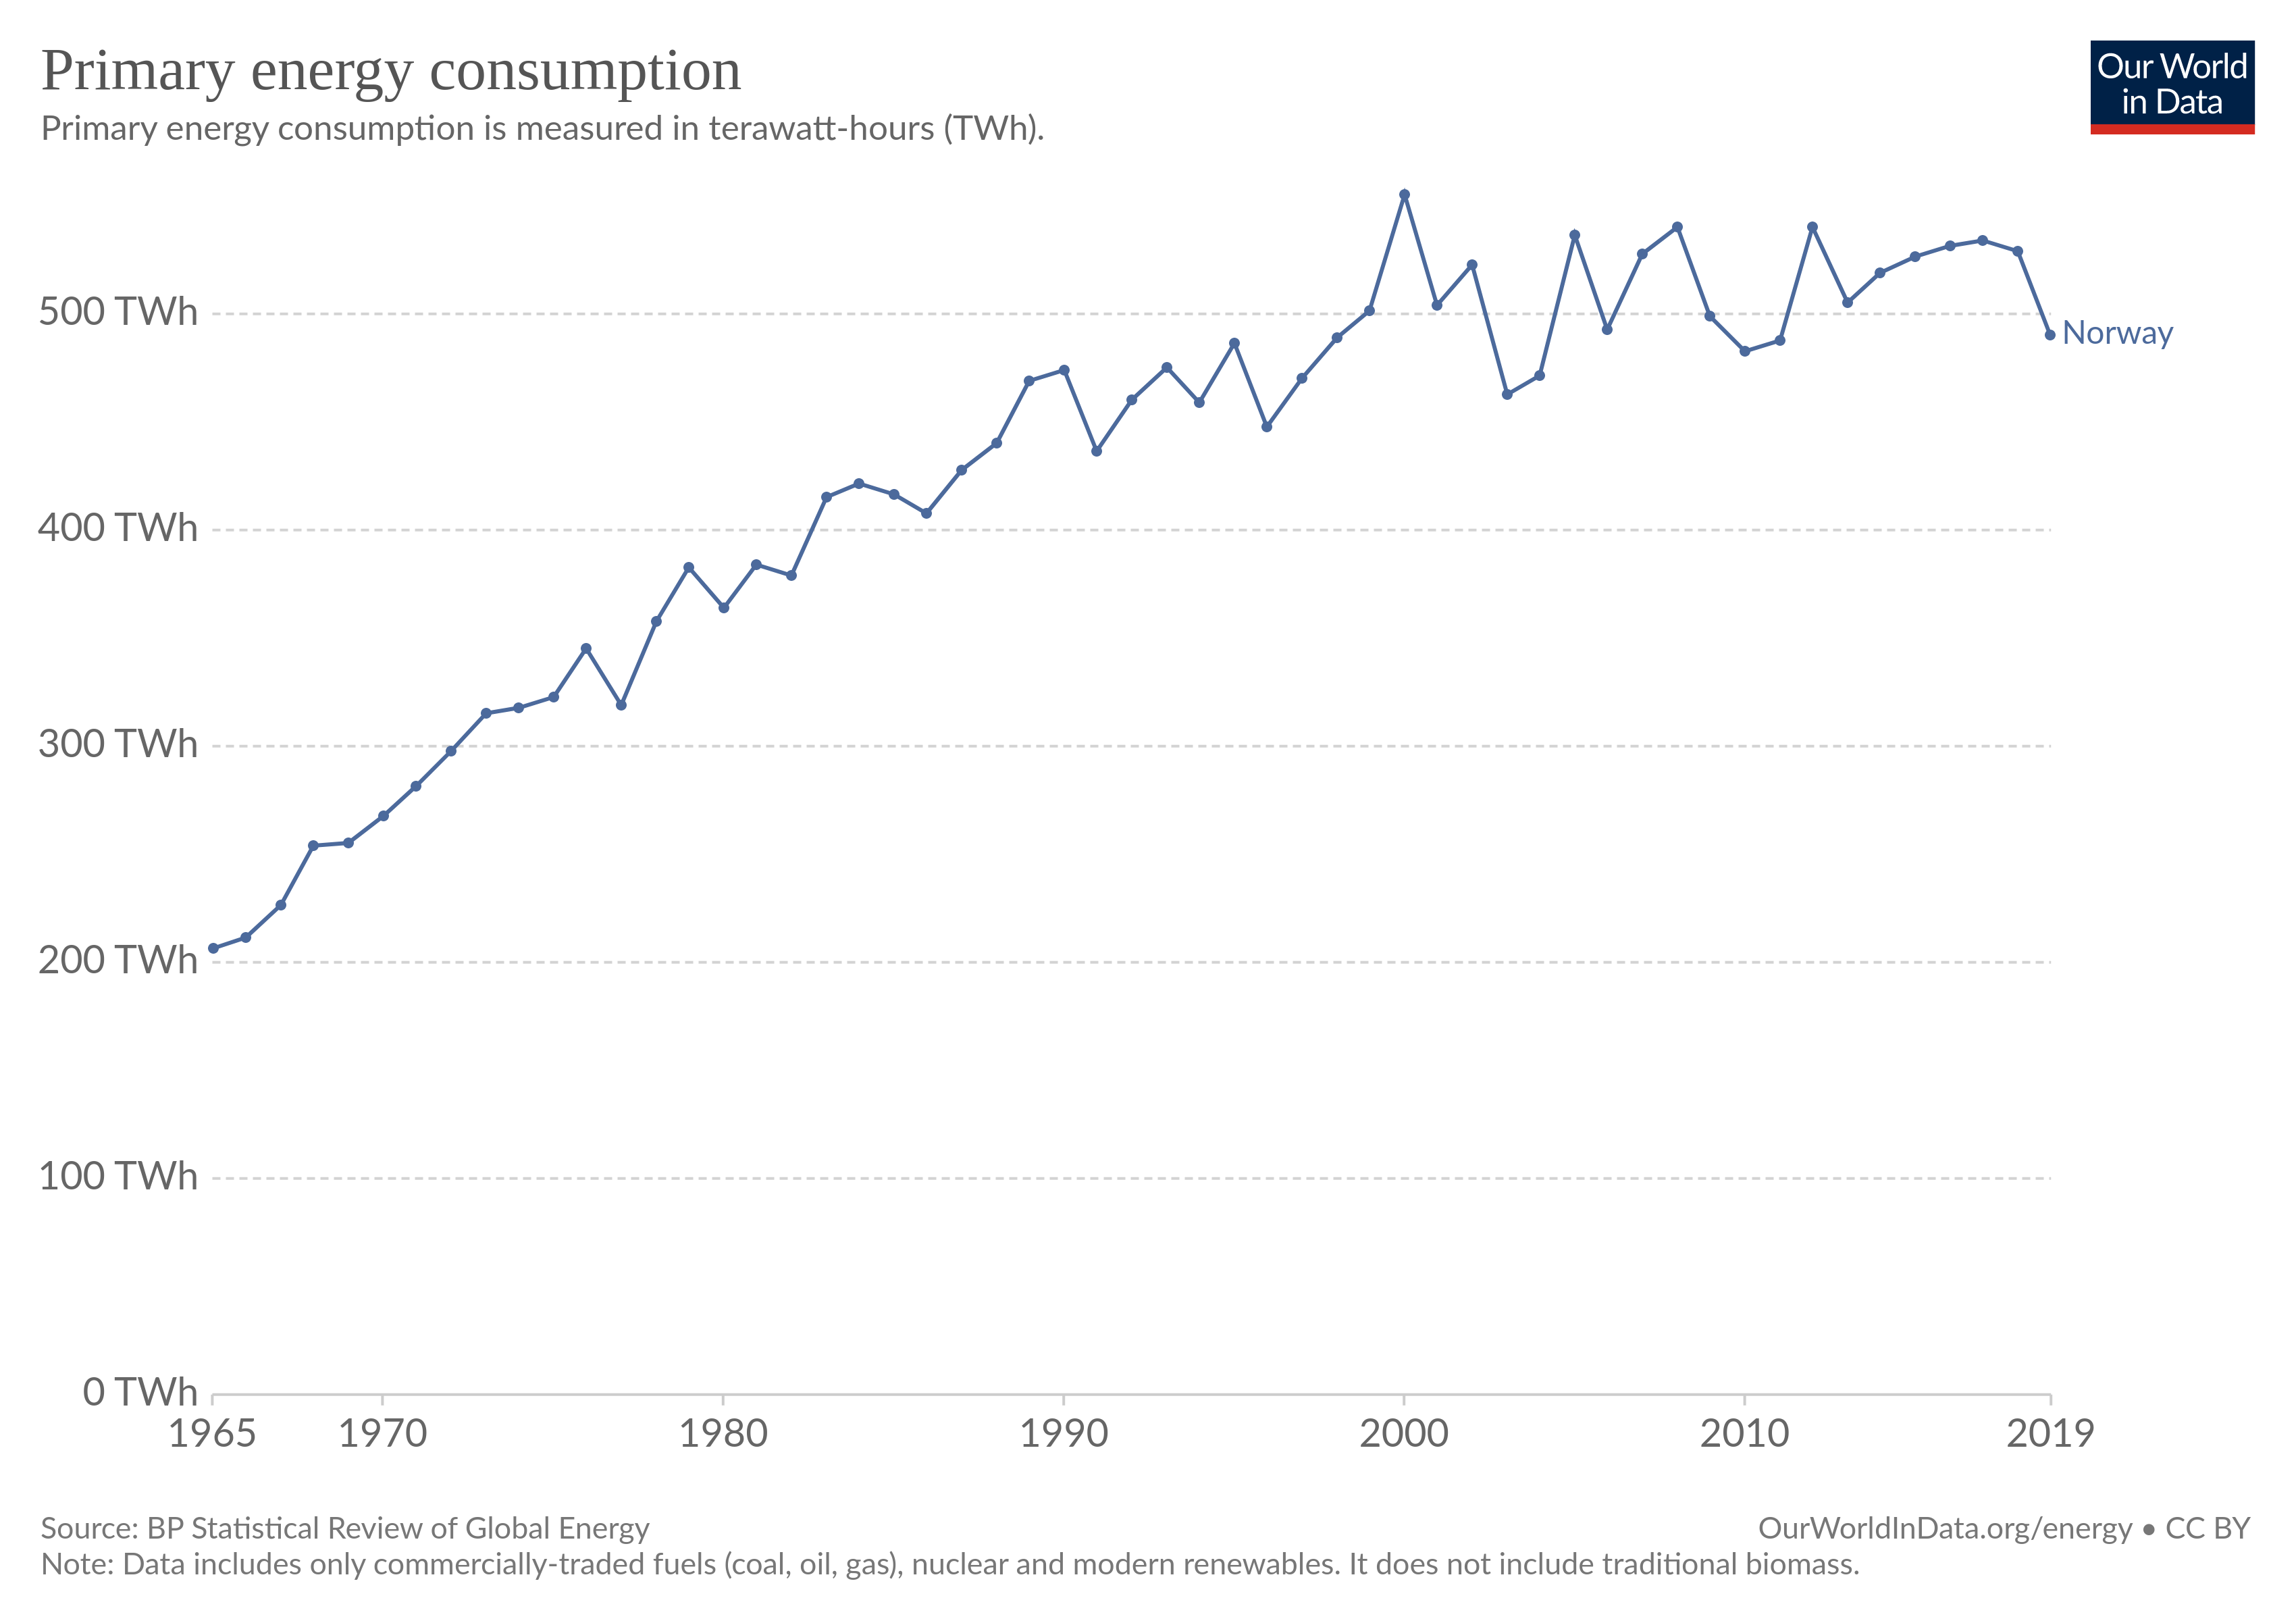
\includegraphics{fig/owid_energy_use_no.png}

\begin{verbatim}
Our World in Data  500 Twh
SB                 250 Twh
\end{verbatim}

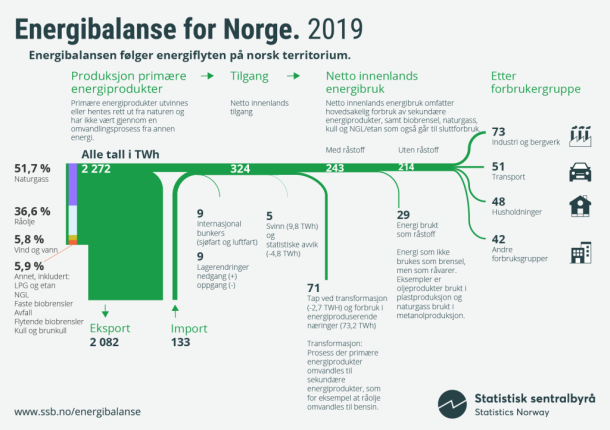
\includegraphics{fig/SSB_2019_Energibalanse_Norge.png}
\href{https://www.ssb.no/energi-og-industri/artikler-og-publikasjoner/reviderte-tall-for-tilgang-og-forbruk-av-energi-og-energiintensiteter}{Source: SSB}

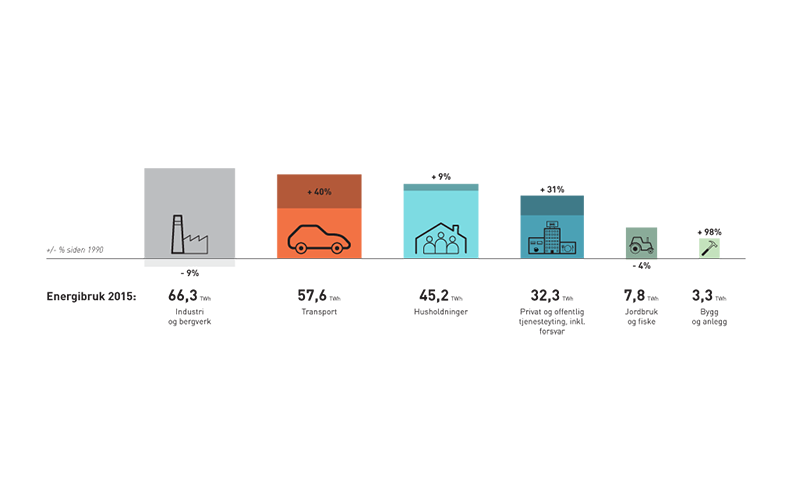
\includegraphics{fig/Utvikling_energibruk_Norge.png}

``Energy use refers to use of primary energy before transformation to other end-use fuels, which is equal to indigenous production plus imports and stock changes, minus exports and fuels supplied to ships and aircraft engaged in international transport.''

Convertion: Kilo of oil equivalent
\href{https://www.unitjuggler.com/convert-energy-from-koe-to-kWh.html}{unitjuggler}

1 koe = 11.63 kWh

\begin{verbatim}
Worldbank/IEA/OECD: Norway 2015 : 5818 koe =  67663 kwh per capita
Our World in data : Norway 2015 :            101181 kwh per capita
\end{verbatim}

\href{https://no.wikipedia.org/wiki/Energi_i_Norge}{Wikipedia: Energi i Norge}

\emph{Statnett: Load Duration Curve}

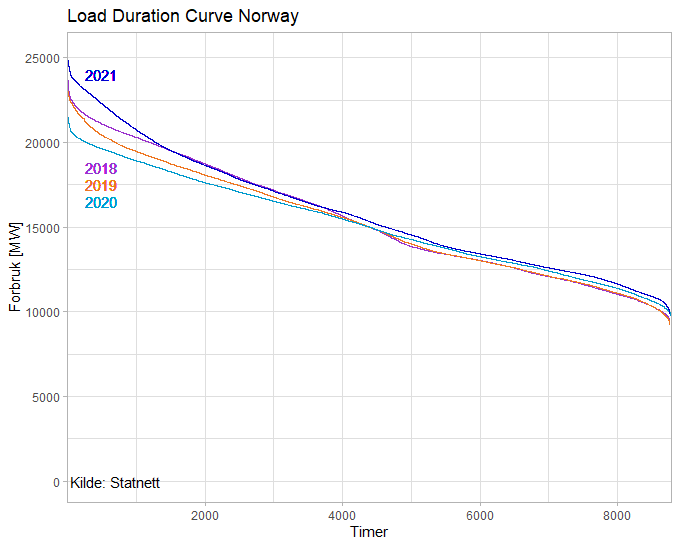
\includegraphics{fig/Load_duration_Norway.png}

50timer med mer enn 24 000 Mwh i forbruk i 2021. Til sammenligning var det kun to timer med tilsvarende forbruk i tre foregående år.

\hypertarget{energy-policy}{%
\section{Energy Policy}\label{energy-policy}}

\emph{Spetalen}

Nordmenn er ikke forbrukerne, vi er eierne av norsk vannkraft. Det er essensen av det hele!
Vi er enige, dette er en nasjonal skandale og flause for Norge.
Investor Øystein Stray Spetalen mener politikerne kan skylde på seg selv for at strømprisene er så høye. Vi er enige!
«Norge har ikke et energiproblem, vi har et politikerproblem»!
-- Vi har dessverre fått inn en kunnskapsløs gjeng. De som har sittet i regjering de siste ti årene har glemt det viktigste, nettopp forvaltningen av kraften vår, sier Spetalen til Klassekampen.
Han mener to grep kan løse situasjonen:
En skatt på 78 prosent på all kraft som eksporteres til utlandet
Norge må melde seg ut av Acer, som er EU-byrået for samarbeid mellom energiregulatorer.
Han mener tilknytningen til EU fratar Norge selvstyre, og han mener unionen er grunnleggende antidemokratisk.
Det har Spetalen svært rett i! Det er totalt svikt i Stortinget! De har glemt hvem de jobber for!

\hypertarget{energy-policy-history}{%
\subsection{Energy Policy History}\label{energy-policy-history}}

\emph{Aam}

I «gamle dager», fram til midten an 1970-tallet, bestemte man hvor mye vannkraft man skulle bygge ut i Norge etter prinsippet om «bestemmende år».

Da sa vi at vi skulle bygge ut så mye vannkraft at vi hadde nok kraft til innbyggerne i ni av ti år. Så fikk vi greie oss som best vi kunne i det tiende som ikke var så mye verre enn det niende. Litt sparing, m.v. og i verste fall litt rasjonering ville være tilstrekkelig for å få «endene til å møtes».

Da var det en utfordring at vi de fleste år hadde vannkraft til overs. Så lagde vi strategier for å få omsetning på overskuddet. Et viktig element var å installere varmekjeler hos store forbrukere som kunne varmes opp med både el og olje og som kunne legge om til oljefyring når det var tørre perioder. Et annet element var å selge fleksibel, billig kraft til industrien -- som kunne kobles ut når det var manko på kraft. Videre knyttet vi landsdelene sammen elektrisk slik at kraftselskap som manglet kraft pga lite nedbør kunne kjøpe kraft av andre som lå i områder som hadde hatt mer nedbør. Til slutt lagde vi utenlandsforbindelser til Sverige og Danmark for å kunne utveksle kraft med utlandet.

Etter hvert lagde Samkjøringen av kraftverkene i Norge et spotmarked der kraftselskaper og industri kunne kjøpe og selge kraft av hverandre. Samkjøringen startet regionsvis fra i 1932 og ble landsomfattende i 1971. Den varte til 1991.

Filosofien i «gamle dager» i de fleste land i Europa, USA og andre land som var avhengig av å bygge ut termisk kraft, var å skape et robust, sikkert og billig kraftsystem. Derfor satset man på diversifisering -- litt kullkraft, litt gasskraft, litt kjernekraft, litt oljekraft og litt vannkraft. Da hadde man en robust risikoavlastning hvis ulike råvarepriser skulle gå opp mye i pris og man kunne spille råvareleverandørene opp mot hverandre. Riktig nok var gassprisen sterkt knyttet til olje, men de andre råvareprisene var til en viss grad uavhengige av hverandre. Dette har fungert bra i «100» år fram til nå og kostnadene for kraftproduksjon har ligget på et «fornuftig» nivå.

For vannkraftlandet Norge var det meget gunstig å utvikle kraftutveksling med Europa. Norge hadde god tilgjengelighet på effekt ved at vannkraftmaskinene enkelt og raskt kunne øke sin produksjon. Videre kunne vi enkelt kjøre vannkraft stasjonene ned og kjøpe inn kraft fra EU for å lagre kjøpet i våre vannkraftmagasin.

Samspillet mellom det termiske Europa og vannkraftlandet Norge var «perfekt match». Norge kunne utnytte muligheten for rask opp og nedkjøring av vannkraftverkene kombinert med å bruke vannkraftmagasinene til korttidslager. Dette tjente vi godt på. Videre kunne vi skaffe oss rimelig termisk kraft på natt og helger i tørrår hvor vi trengte å importere kraft. EU fikk tilgang til toppeffekt på hverdagene til en billigere penge enn å produsere toppeffekten selv. Utbyggingen av kraftkabler til Danmark og Nederland var drevet av slike tanker.

Norge var det første landet til å liberalisere kraftforsyningen i 1990/91. Det var \href{https://no.wikipedia.org/wiki/Eivind_Reiten}{Senterpartimannen Eivind Reiten} som var Olje-og energiminister 89/90 og miljøet rundt Handelshøyskolen i Bergen (blant andre Einar Hope) som var aktive pådrivere for å innføre en \href{https://no.wikipedia.org/wiki/Energiloven}{ny energilov} som skilte ut kraftproduksjon som konkurranseutsatt virksomhet. Dette ble senere fulgt opp i Norden og i EU som har som mål å lage best mulig felles marked for kraft og gass i hele EU.

Den norske stat tjener mye på salg av dyr gass til Europa. Det at Norge har lav magasinfylling i Sør-Norge gjør at kraftprisen der blir spesielt preget av kraftprisen i Europa. Norske kraftprodusenter får godt betalet for de nedskrevne vannkraftanleggene med dagens høye priser. Vanlige borgerne i Norge må imidlertid betale den høye prisen i det felles europeiske kraftmarkedet hvor prisen på dyr gass og CO₂ er styrende nå.

Samspillet mellom det norske og nordiske kraftsystemet og EU er beskrevet blant annet i rapporten \href{https://www.statnett.no/globalassets/for-aktorer-i-kraftsystemet/planer-og-analyser/nordic-grid-development-perspective-2021.pdf}{Nordic Grid Development Perspective 2021 (pdf)}, fra de nordiske nettselskapene (TSO'ene) og DNV-rapporten \href{https://www.dnv.com/Publications/energy-transition-norway-2021-212201}{Energy Transition Norway 2021}

Regjeringen har kommet borgerne i møte med \href{https://www.nrk.no/norge/regjeringen-med-pressekonferanse-om-stromsituasjonen-1.15728336}{krisepakken for strøm}.
og vil sette ned en \href{https://www.regjeringen.no/no/aktuelt/energiforskningskonferansen/id2879520/}{energikommisjon}.

\href{https://blogg.sintef.no/sintefenergy-nb/hva-i-all-verden-skjer-med-kraftmarkedet/}{Aam (2021) Hva i all verden skjer med kraftmarkedet?}

\emph{Tamburstuen}

Dette er en strukturell krise. Og den må løses med radikale strukturelle, politiske tiltak, for dette var i k k e hensikten med energiloven:

\begin{itemize}
\item
  Ta kontroll over Nordpool og la Statnett og norske kraft- og nettselskap stå for omsetningen av strøm. Det er ingen mening i at et utenlandseid børs-selskap skal kunne tjene milliarder på omsetningen av norsk strøm og ta enorme utbytter ut av Norge
\item
  la brukerne kjøpe strømmen fra denne nye enheten - basert på et prinsipp om kost pluss. På denne måten får produsentene og netteierne pløyd direkte tilbake en rimelig fortjeneste som brukes for oppgraderinger av kraftverk og nett. Det er et potensiale for en vesentlig økning av produksjonen i eksisterende vannkraftverk, uten naturinngrep.
\item
  dette betyr at de såkalte strømselskapene forsvinner fra markedet
\item
  sett et krav om minimum magasinfylling hele året - og sørg for at dette etterleves. Vår magasinkapasitet utgjør 70\% av vår årlige produksjon av vannkraft og er bygget opp nettopp for å lagre energi -- denne kapasiteten er unik i Europa
\item
  reforhandle avtalene om utenlandskablene slik at Norge har nasjonal kontroll med hva som skal gå ut og inn av strøm
\item
  Pålegg Statnett å investere i stamnettet slik at en unngår flaskehalsene som skaper de store prisforskjellene innenlands
\item
  Dropp elektrifiseringen av sokkelen - gi oljeselskapene et lite skatteincentiv og krev at avgassene fra gassturbinene er renset innen en gitt frist
\item
  Lag beredskap - lovmessig og finansielt - for å sikre at kraftverk og nett forblir på norske hender
\item
  Bruk eierskapet i Statkraft og Statnett til å sørge for at disse to selskapene oppfyller sine oppdrag i Norge
\item
  Styrk arbeidet med reell energiøkonomisering, og start arbeidet med geoenergi/jordvarme og med bioenergi -- norske skoger flyter over av biomasse
\end{itemize}

\emph{Tamburstuen 2}

Trygve Tamburstuen gir her en opplysende og oppsiktsvekkende oversikt over hvordan vi er havnet i det nåværende kraftkaoset. Han gir også en helt nødvendig og presis beskrivelse av hva som gjøres for å få kontroll over kraftsituasjonen.
KRONIKK Trygve Tamburstuen, styreleder i flere selskaper:
GLADE DAGER I NEW YORK: Nasdaq-børsen har med sine allierte arbeidet for bygging av flest mulig grenseoverskridende strømforbindelser, fordi de med dette kontrollerer krafthandelen i Europa. De handler med alle kjente spekulasjonsobjekter, og vil selvsagt tjene mest mulig på hver transaksjon, skriver Trygve Tamburstuen.FOTO: BRYAN R. SMITH, AFP/NTB
Energilovens intensjon var at brukerne kunne velge den leverandør som tilbyr lavest pris. Det store politiske feilgrepet var å gjøre strøm til en vare i et marked som ingen kontrollerer. Det var en reform ingen ba om, men et nettverk av sosialøkonomer drev fram dereguleringen, i en tid der konkurranseutsetting var det store mantraet.
For å sikre en effektiv omsetning ble Statnett -- tidligere Samkjøringen -- satt til å drive en kraftbørs, og Statnett Marked ble etablert i 1993. Senere kom de nordiske og baltiske nettselskapene inn som eiere. Vi var interessert i å importere strøm fra naboland på kveld og natt, mens vi kunne eksportere på dagtid og utnytte magasinkapasiteten til å lagre strøm.
I 2001 byttet Statnett Marked navn til NordPool, og det ble etablert flere datterselskaper. De kommersielle aktørene, inkludert Statnett, så at utenlandskabler og sammenkopling av kraftbørsene ville gjøre det nordiske kraftmarkedet integrert både fysisk og finansielt med det europeiske kraftmarkedet.
Den finansielle krafthandelen omfatter handel med finansielle instrumenter som brukes som rene spekulasjonsobjekter. NordPool bygget opp en egen plattform for slik handel med kraft og CO₂-sertifikater. Og da starter børsifiseringen og den totale finansialiseringen av kraftmarkedet: I 2008 selger NordPool sin andel i kraftbørsen og mesteparten av sin øvrige virksomhet til Nasdaq OMX (Nasdaq er New York-børsen) for rundt 2.4 milliarder kroner.
NordPool, som da var 50 prosent eid av Statnett, selger altså det viktige aktivum som den finansielle kraftbørsen er, uten at Stortinget behandler salget!
Nasdaq OMX har helt klare ambisjoner. I dag styrer de kraftomsetningen i over 20 land i Europa. Nasdaq har to datterselskaper i Norge som nyter godt av dette: Nasdaq OMX Oslo omsatte i 2020 for 112 millioner og fikk et årsresultat på 29 millioner. Nasdaq Clearing omsatte for 195 millioner med et årsresultat på 107 millioner. Fortjenestemarginen i denne delen av krafthandelen er altså på 44 prosent.
Nasdaq og deres allierte har selvsagt bevisst arbeidet for bygging av flest mulig grenseoverskridende strømforbindelser, fordi de med dette kontrollerer krafthandelen i Europa. De handler med alle kjente spekulasjonsobjekter, kort- og langsiktig, opsjoner, og vil selvsagt tjene mest mulig på hver transaksjon.
Jeg omtaler ikke strømselgerne her, men en etablering av kraftbørsen er jo den mekanismen som åpnet for at 130 -- i stor grad utenlandseide -- strømselgere i dag operer i det norske markedet. Et ferskt eksempel er at Kintech Energy Spot, et datterselskap av et amerikansk selskap, har påført Bardu kommune et tap på 13 millioner ved å selge konsesjonskraft for kommunen!
Så fullføres skandalen i 2019: da selger Statnett og partnerne 66 prosent av den fysiske kraftbørsen kalt NordPool Holding 2 AS, til den Nederland-baserte børseieren Euronext, som også eier Oslo Børs.
I 2020 har Euronext et årsresultat i Norge på 575 millioner og tar ut 392 millioner i utbytte. NordPool Holding tar ut 75 millioner og TSO Holding, som eier de resterende 34 prosent av kraftbørsen, tar ut 480 millioner i utbytte -- 30 prosent av dette tilfaller Statnett. NordPool Holding 2 AS eier NordPool AS og European Market Coupling Operator AS (navnet sier vel det meste).
Prisen for de 66 prosent var 640,2 millioner, som må betegnes som et rent billigsalg i lys av den enorme strategiske verdien denne plattformen har. Igjen skjer salget uten at Stortinget behandler det. Sigbjørn Gjelsvik (Sp) stiller et spørsmål til statsråd Freiberg (Frp), men blir avvist og saken følges aldri opp.
«Nasdaq har helt klare ambisjoner.»
Fra å ha full statlig kontroll over både den fysiske og finansielle krafthandelen er det altså nå Nasdaq og Euronext -- to av de største internasjonale børseierne -- som kontrollerer ikke bare den norske kraftomsetningen, men også den europeiske. Og de har fått kontrollen for veldig beskjedne beløp, noe som bør rette søkelyset mot styre og daglig ledelse av Statnett i perioden.
Vi er altså nå del av et fullintegrert europeisk kraftmarked. Samtidig har energipolitikken i EU slått helt feil, og utsiktene er dårlige: Europa har i overskuelig framtid lav selvforsyningsgrad på fornybar energi. Får vi ikke kontrollen over egen kraft, vil høye priser til husholdninger og industri i Norge forbli en permanent tilstand.
Kontrollen kan vi få tilbake ved å:
ta tilbake kraftbørsen, både den finansielle og den fysiske, og fjerne strømselgerne fra markedet
reforhandle avtalene om kraftutveksling slik at vi selv kontrollerer flyten i kablene
bestemme et transparent kostnadsregime for prisingen av kraft i Norge
instruere Statnett til å investere i stamnettet i Norge for å fjerne flaskehalsene.
Statnetts investeringer i de nye kraftkablene til Tyskland og Storbritannia er 18 milliarder. Hittil har strømmen bare gått én vei i disse kablene, og det er ingen grunn til å forvente at landene i overskuelig framtid vil kunne levere strøm til Norge -- dette er altså rene eksportledninger.
Vi sitter med uhyre sterke forhandlingskort:
Norge dekker 25 prosent av Europas totale gassforbruk, som transporteres direkte i rør (USAs fabling nå om å redde Europas gassbehov med LNG på skip virker helt absurd).
To tredeler av Norges gassreserver er ikke produsert ennå -- vi er altså en langsiktig solid leverandør.
Tyskland tar imot mest -- 50 prosent i 2020 -- mens Storbritannia tok 26 prosent. Dette er altså også de samme markedene som bare importerer norsk strøm og ikke leverer noe tilbake".

\href{https://www.dagensperspektiv.no/2021/el-markedet-ma-endres-strukturelt}{Tamburstuen (2021) El-markedet må endres strukturelt}

\hypertarget{serbia}{%
\chapter{Serbia}\label{serbia}}

\emph{Tooze}

\textbf{Mining Lithium in Serbia}

I found this \href{https://www.ft.com/content/707e7a39-f357-484a-8efc-b0b7dc475600}{FT} piece on the contested \href{https://www.riotinto.com/en/operations/projects/jadar}{Rio Tinto lithium} development in Jadar, Serbia intriguing, but also question begging.

Asking the hive mind of twitter for more information, elicited this very sensible intervention by Aleksandar Milosevic on danas.rs Stick it through google translate.

\begin{quote}
the dilemma to be decided is 1,000 well-paid jobs and about 30 million euros of annual state revenue (plus 2,000 jobs on construction and partly engaging domestic suppliers in a project worth over two billion euros), and against the relocation of 50 families, the destruction of some 400 hectares of land and the creation of tailings to the detriment of local flora and fauna. A potential battery factory with its jobs and taxes or a different calculation of state revenues changes the ratio of gains and losses. So, we decide on that. And not about whether we are for Vučić or not.
\end{quote}

\href{https://adamtooze.substack.com/p/serbian-lithium-mother-courage-and}{Tooze}

\hypertarget{united-states}{%
\chapter{United States}\label{united-states}}

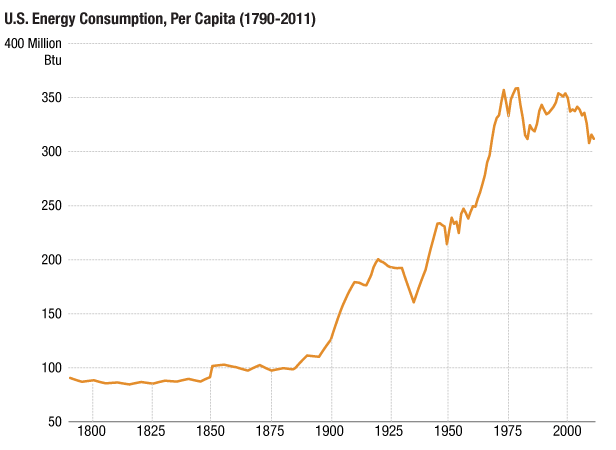
\includegraphics{fig/us_energy_consumption_pc_1790-2011.png}

\textbf{Links US}

\href{https://innovationfrontier.org/geothermal-everywhere-a-new-path-for-american-renewable-energy-leadership/}{Geothermal Everywhere: A New Path for American Renewable Energy Leadership}

\hypertarget{part-appendices}{%
\part{Appendices}\label{part-appendices}}

\hypertarget{appendix-appendices}{%
\appendix}


\hypertarget{about}{%
\chapter{About}\label{about}}


\includegraphics{fig/me.jpg}

\emph{Dyre Haugen} and \emph{Dyrehaugen} is Webian for \emph{Jon Martin} -
self-owned Globian, Webian, Norwegian and Canarian with
a background from industrial research policy, urban planning and
economic development consulting on global, regional and urban scales.
I am deeply concerned about the (insane) way
humanity (i.e.~capitalism) interfere with nature.
In an effort to gain insights in how and why this happens
stuff is collected from around the web and put together
in a linked set of web-sites.
The sites are operated as personal notebooks.
However, these days things can be easily published to the
benefit of others concerned with the same issues.
But be aware - this is not polished for presentation or
peer-reviewed for exactness.
I offer you just to have a look at my `work-desk' as it appears in the moment.
Any comment or suggestion can be mailed to \href{mailto:dyrehaugen@gmail.com}{\nolinkurl{dyrehaugen@gmail.com}}
You can follow me on twitter as @dyrehaugen.
Thanks for visiting!

\hypertarget{links}{%
\chapter{Links}\label{links}}

\textbf{Current Dyrehaugen Sites:}

\begin{itemize}
\tightlist
\item
  \href{https://dyrehaugen.github.io/rcap}{rcap - On Capitalism} \href{http://localhost/rcap}{(loc)}
\item
  \href{https://dyrehaugen.github.io/rclm}{rclm - On Climate Change} \href{http://localhost/rclm}{(loc)}
\item
  \href{https://dyrehaugen.github.io/recs}{recs - On Economics} \href{http://localhost/recs}{(loc)}
\item
  \href{https://dyrehaugen.github.io/rngy}{rfin - On Finance} \href{http://localhost/rfin}{(loc)}
\item
  \href{https://dyrehaugen.github.io/rngy}{rngy - On Energy} \href{http://localhost/rngy}{(loc)}
\item
  \href{https://dyrehaugen.github.io/renv}{renv - On Environment} \href{http://localhost/renv}{(loc)}
\item
  \href{https://dyrehaugen.github.io/rsts}{rsts - On Statistics} \href{http://localhost/rsts}{(loc)}
\item
  \href{https://dyrehaugen.github.io/rurb}{rurb - On Urbanization} \href{http://localhost/rurb}{(loc)}
\item
  \href{https://dyrehaugen.github.io/rvar}{rvar - On Varia} \href{http://localhost/rvar}{(loc)}
\item
  \href{https://dyrehaugen.github.io/rwsd}{rwsd - On Wisdom} \href{http://localhost/rwsd}{(loc)}
\end{itemize}

\textbf{Blogs:}

\begin{itemize}
\tightlist
\item
  \href{https://dyrehaugen.github.io/rde}{rde - Blog in English} \href{http://localhost/rde}{(loc)}
\item
  \href{https://dyrehaugen.github.io/rdn}{rdn - Blog in Norwegian} \href{http://localhost/rdn}{(loc)}
\end{itemize}

\textbf{Discontinued:}

\begin{itemize}
\tightlist
\item
  \href{https://dyrehaugen.github.io/jdt}{jdt - Collection (Jekyll)} \href{http://localhost/jdt}{(loc)}
\item
  \href{https://dyrehaugen.github.io/hdt}{hdt - Collection (Hugo)} \href{http://localhost/hdt}{(loc)}
\end{itemize}

\textbf{Not listed:}

\begin{itemize}
\tightlist
\item
  (q:) dhe dhn jrw56
\item
  (z:) rcsa rpad rstart
\end{itemize}

\hypertarget{news}{%
\chapter{NEWS}\label{news}}

\hypertarget{silicon-batteries}{%
\section{220505 Silicon Batteries}\label{silicon-batteries}}

\emph{Canary Media}

The German carmaker led a \$400 million investment in American startup Group14 Technologies, which makes advanced batteries using silicon. Adding silicon to the anode (one of the key parts of a battery cell) could significantly improve the driving range and charge time of electric vehicles, two crucial metrics for their broader acceptance. But the technology is generally expected to be years away from widespread commercial adoption.

Group14 aims to move up that timeline --- its silicon anodes are on track to get into electric vehicles by 2023, CEO and co-founder Rick Luebbe told Canary Media.

``Silicon batteries are here,'' he said. \hspace{0pt}``The technology is proven. Now it's about scaling to meet the demand.''

Group14 already has a factory outside of Seattle that produces 120 tons of silicon-carbon composite per year. But the new Series C funding will bankroll construction of another factory in central Washington, which will produce enough battery materials for 600,000 EVs per year when it's fully operational in late 2023. A South Korea facility jointly developed with SK Group is coming online this year.

Silicon anodes hold more energy than conventional graphite anodes. That inspired scientists to replace some or all of the graphite in the anode with silicon.
Get Caught Up

But this improvement doesn't come without problems. Silicon expands and contracts as the battery charges and discharges, and those fluctuations can damage the battery. The trick for companies including Group14 is to harness the energy capacity of silicon while minimizing the damage it causes.

Group14's recipe, dubbed SCC55, uses \hspace{0pt}``hard carbon-based scaffolding'' to keep that silicon \hspace{0pt}``in the most ideal form -- amorphous, nano-sized, and carbon-encased,'' according to the company's website. In other words, the silicon sits in a miniscule scaffolding structure where it has room to expand and contract without weakening the structure of the anode, Luebbe explained.

Achieving an ideal anode requires years of complicated laboratory science. Group14 grew out of a company called EnerG2 that focused on nanoengineering synthetic carbons; that parent company was sold to BASF, and then Group14 was spun out in 2015 to apply that technological approach to silicon anodes.

Such scientific complexity usually harshes the vibes of venture investors hyped up on the prospect of quick software returns. But the prize in this case was particularly alluring. Silicon enthusiasts, Group14 included, claim that adding it to anodes can deliver 50 percent more energy density than today's batteries. That could materialize as an EV that goes much farther on a single charge, or one that goes the same distance with a smaller, cheaper battery.

\href{https://www.canarymedia.com/articles/electric-vehicles/porsche-investment-could-unlock-a-25-boost-in-ev-battery-density}{Canary (2022)Porsche investment could unlock up to a 50\% boost in EV battery density}

\hypertarget{europes-energy-crisis}{%
\section{220116 Europe's Energy Crisis}\label{europes-energy-crisis}}

\emph{Birol}

In Europe, governments should make natural gas storage part of their security of supply risk assessments, at both a national and regional level, including risks linked to the control of storage by entities from non-EU countries. And regulations should be improved to ensure that storage levels are adequate to cover end-user needs, with mandatory minimum storage obligations assigned to all commercial operators with gas retail portfolios. In addition, provisions on transparency and congestion management can help to ensure optimal utilisation of available storage capacity.

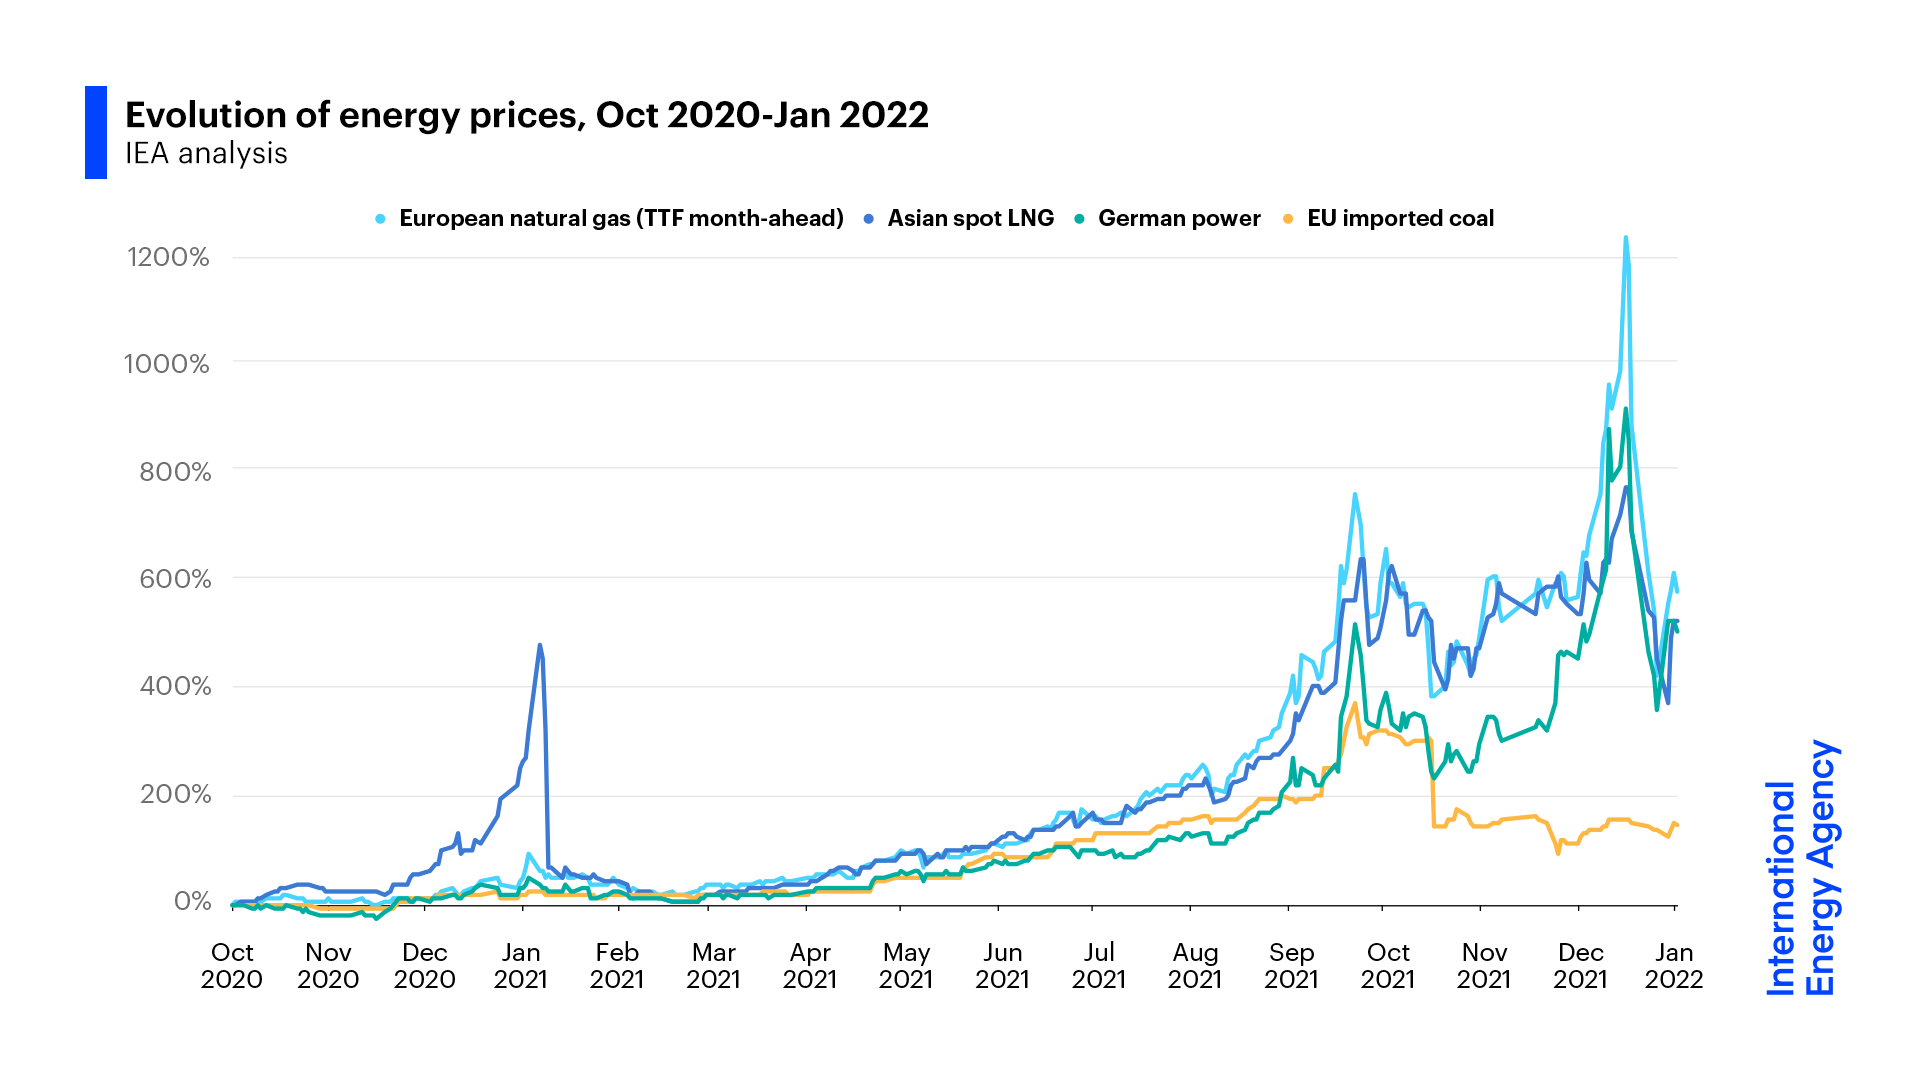
\includegraphics{fig/Energy_Prices_Oct2020-jan2022_IEA.png}

On a global level, scaling up domestically sourced low-carbon energy supplies provides an opportunity to bring down emissions while at the same time tackling energy security issues related to fossil fuel imports and market volatility. However, potential energy security vulnerabilities do not disappear in a renewables-rich and more electrified energy system. Policy makers need to pay close attention to new clean energy supply chains, in particular the geographical concentration of many \href{https://www.iea.org/reports/the-role-of-critical-minerals-in-clean-energy-transitions}{critical minerals} -- such as lithium, cobalt and rare earth elements -- that are crucial components of many clean energy technologies.

In my view, today's situation underlines the fact that energy systems face significant risks if they rely too much on one supplier for a key element. Today, it is natural gas; tomorrow, it could be something else, such as lithium.

\href{https://www.linkedin.com/pulse/europe-world-need-draw-right-lessons-from-todays-natural-fatih-birol/}{Birol (2022) Europe and the world need to draw the right lessons from today's natural gas crisis}

\hypertarget{novel-lithium-carbon-battery-chemistry}{%
\section{211207 Novel lithium-carbon battery chemistry}\label{novel-lithium-carbon-battery-chemistry}}

A prototype battery-powered moped that can recharge in as little as 90 seconds could be on the road next year.

The vehicle will be used to test a novel lithium-carbon battery developed by U.K.-based Allotrope Energy and unveiled in September by Mahle Powertrain, a British subsidiary of one of the world's largest automotive suppliers.

The fast-charging capacity is a result of the lithium-carbon battery's high specific power, which tops 15 kilowatts per kilogram, according to Allotrope. This compares to a maximum of around 10 kW per kilogram for other lithium-ion chemistries.

The fact that lithium-carbon batteries had not already been developed might seem odd given the battery industry's keenness for novel chemistries. The holdup was because an essential component of the chemistry, nanoporous carbon, only recently began being used in battery development.

In theory, the battery could be fully charged in just 60 seconds. The 90-second charging time is due to the limitations of charging infrastructure rather than the battery.

The reason why it's a 90-second charging is a buffered chargepoint. The charger has a battery inside it and the battery dumps its energy into the moped.

For the larger batteries used in electric cars, there simply isn't enough grid capacity to cope with lithium-carbon batteries. That's why it's unlikely the chemistry will be scaled up for larger vehicles.

Another advantage of the lithium-carbon chemistry is that it does not use cobalt or nickel, two elements that pose supply-chain concerns in some other lithium-ion battery types.

\href{https://www.canarymedia.com/articles/electric-vehicles/prototype-of-electric-moped-with-90-second-charge-time-set-to-hit-the-streets-in-2022}{Canary Media}

\hypertarget{renewables-passing-nuclear}{%
\section{210710 Renewables passing Nuclear}\label{renewables-passing-nuclear}}

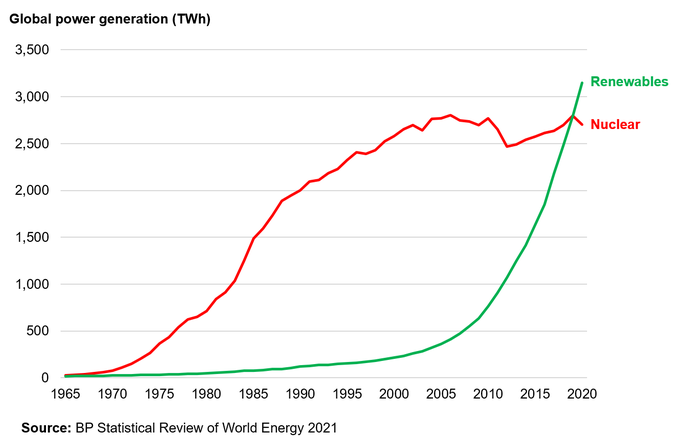
\includegraphics{fig/renewables_passing_nuclear.png}

\href{https://www.bp.com/en/global/corporate/energy-economics/statistical-review-of-world-energy.html}{BP Statistical Review of World Energy}

\hypertarget{equinor-triple-uk-hydrogen}{%
\section{210629 Equinor triple UK hydrogen}\label{equinor-triple-uk-hydrogen}}

Norway's state oil company Equinor will triple its UK hydrogen output, after setting out plans to build the world's biggest hydrogen production plant with carbon capture and storage technology near Hull.

Equinor plans to produce clean-burning ``blue hydrogen'' to supply the Keadby gas power plant in Lincolnshire, owned by energy company SSE, making it the world's first full-scale power plant to burn pure hydrogen to generate electricity.

Anders Opedal, the chief executive of Equinor, said on Monday that the company plans to produce another 1,200MW of blue hydrogen in the Humber area to help supply the Keadby hydrogen power plant.

\href{https://www.theguardian.com/business/2021/jun/29/equinor-to-triple-uk-hydrogen-output-with-new-plant-near-hull}{Guardian}

\hypertarget{crane-battery}{%
\section{210604 Crane Battery}\label{crane-battery}}

Energy Vault stores clean electricity by stacking blocks of concrete.

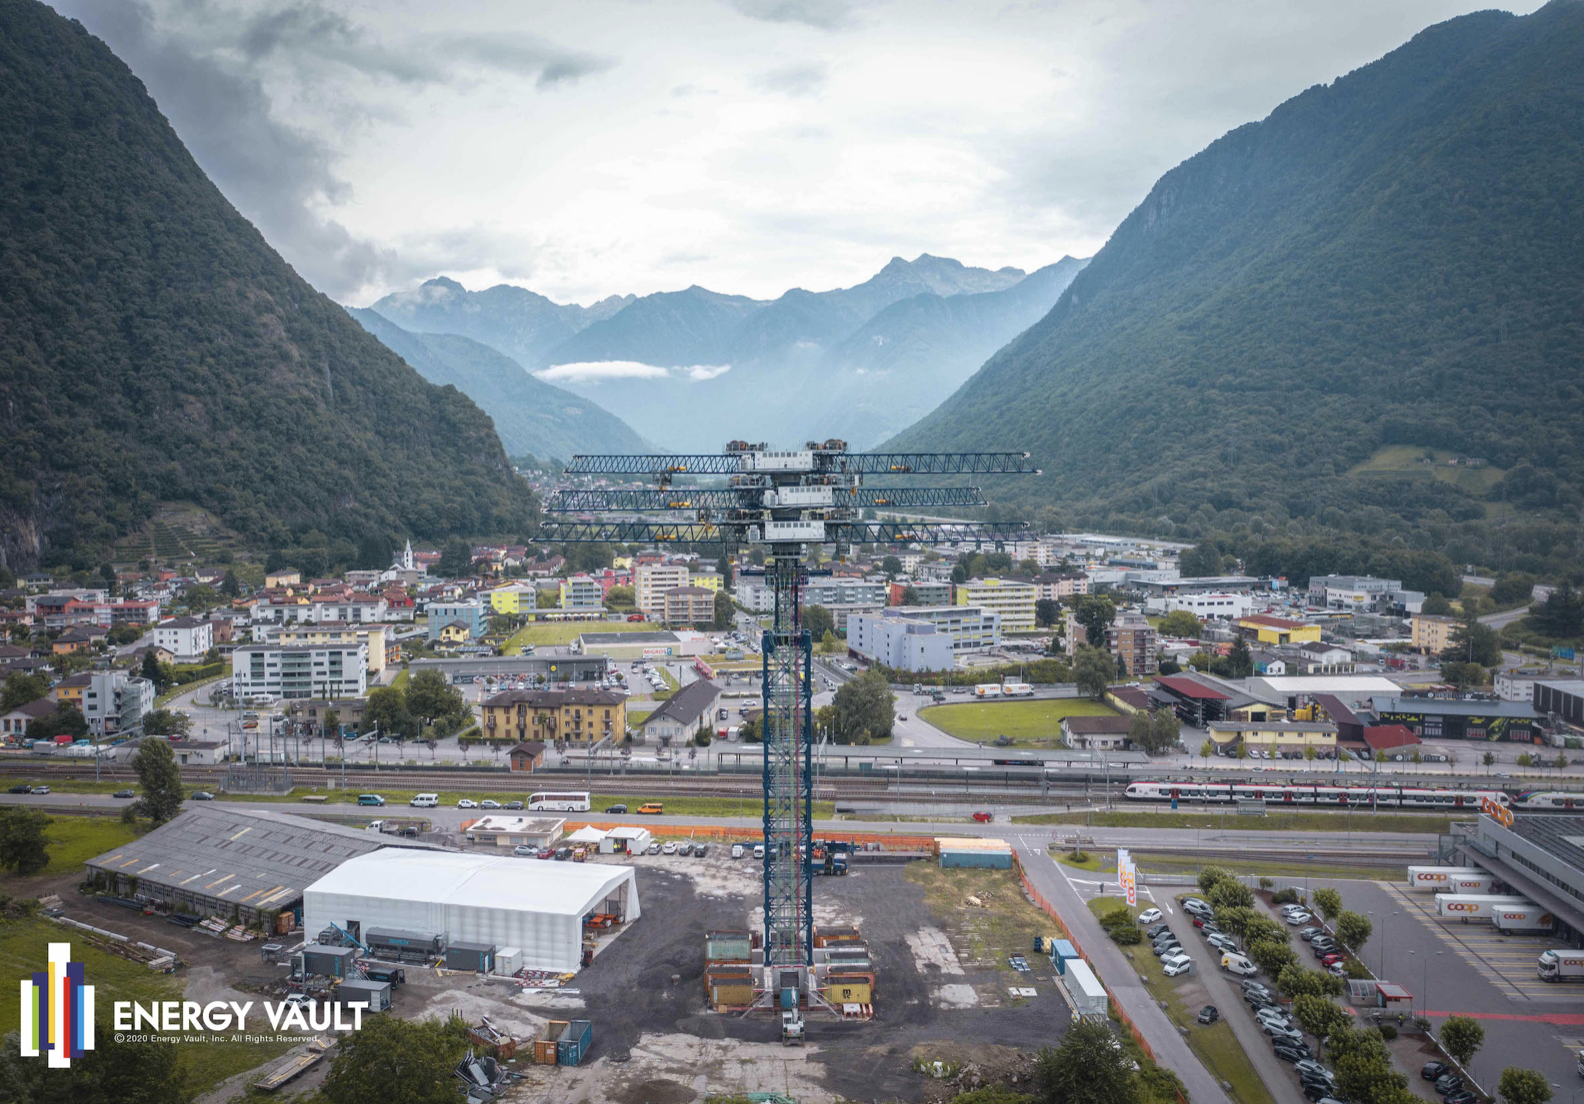
\includegraphics{fig/crane_battery.png}

Energy Vault completed its first commercial-scale project in July 2020, when it connected a 5 megawatt/ 35 megawatt-hour block-stacking tower to the Swiss grid, the company said. The system's six crane arms use electricity to hoist purpose-built concrete blocks and stack them into a tower; rapidly lowering the blocks discharges electricity.

\href{https://www.canarymedia.com/articles/energy-vault-nabs-investment-from-saudi-aramco-for-block-stacking-storage/}{CanaryMedia}

\hypertarget{heatcrete-thermal-storage}{%
\section{210427 HeatCrete Thermal Storage}\label{heatcrete-thermal-storage}}

Norway-headquartered EnergyNest makes its own branded ThermalBattery product which essentially stores heat in a patented form of concrete, which it has dubbed Heatcrete. A heat transfer fluid (HTF) at high temperatures passes through steel pipes cast into the `battery', in technology that the company claims enables storage of energy at very low CapEx cost, using low-cost materials in a simple design. EnergyNest has previously said the Heatcrete materials can last 30 to 50 years of use without degradation.

An investment worth €110 million (US\$131.5 million) has been agreed by `thermal battery' manufacturer EnergyNest which would make infrastructure equity investor Infracapital its biggest shareholder.

Infracapital's investment will be used by the thermal energy storage company towards delivering financed turnkey energy storage solutions in a range of international regions,

EnergyNest made its first large-scale deployment in a research and demonstration project in Abu Dhabi with Masdar Institute, a 1MWth system developed between 2013 and late 2015. As with providers of other novel energy storage technologies, the company has been seeking to commercialise its products and offerings over the past few years and claimed that 2020 was its strongest year to date.

In January last year Energy-Storage.news reported that the company was deploying a multi-megawatt solution at a brick making factory in Austria and in June announced a partnership with Siemens Energy to develop commercialised solutions --- the pair had already worked together previously at the Abu Dhabi pilot project. A project with Italian energy major Eni at a solar energy plant is also already underway and another with Norwegian chemical company Yara is in development to produce steam for industrial use.

\href{https://www.energy-storage.news/news/thermal-energy-storage-startup-energynest-secures-us130-million-investment}{EnergyStorage}

\href{https://energy-nest.com/technology/}{EnergyNest}

\hypertarget{gas-is-over}{%
\section{210121 ``Gas is over''}\label{gas-is-over}}

Europe needs to acknowledge that its future is no longer with fossil fuels, said the President of the European Investment Bank as he presented the bank's 2020 results on Wednesday (20 January).

``To put it mildly, gas is over,'' Dr Werner Hoyer said at a press conference on the EIB's annual results.

\href{https://www.euractiv.com/section/energy-environment/news/gas-is-over-eu-bank-chief-says/}{EIB Gas is over}

  \bibliography{book.bib,packages.bib}

\end{document}
